%%%---PREAMBLE---%%%%%%%%%%%%%%%%%%%%%%%%%%%%
\documentclass[oneside,12pt,final]{sty/ucthesis-CA2012}
\pdfoutput=1

%--- Packages ---------------------------------------------------------
\usepackage[lofdepth,lotdepth,caption=false]{subfig}
\usepackage{fancyhdr}
\usepackage{hyperref}
\usepackage{amsmath, amssymb, graphicx}
\usepackage{xspace}
\usepackage{braket}
\usepackage{color}
\usepackage{subfig}
\usepackage{setspace}
\usepackage{chngcntr}
\usepackage{siunitx}
\usepackage[numbers,sort&compress]{natbib}
\usepackage{adjustbox}
\usepackage{makecell}
\usepackage{glossaries}

	
%---New Definitions and Commands------------------------------------------------------
\def\p{\partial}
\def\im{\mrm{im}}
\def\Tr{\mrm{Tr}}
\def\Z{\mbb{Z}}
\def\R{\mbb{R}}
\def\C{\mbb{C}}
\def\half{\frac{1}{2}}
\def\filler{\phantom{fillerfillerfiller}}
\newcommand{\be}{\begin{equation}}
\newcommand{\ee}{\end{equation}}
\newcommand{\mbb}[1]{\mathbb{#1}}
\newcommand{\mrm}[1]{\mathrm{#1}}
\newcommand{\mcal}[1]{\mathcal{#1}}
\newcommand{\mbf}[1]{\mathbf{#1}}
\newcommand{\ph}[1]{\phantom{#1}}
\newcommand{\udten}[3]{#1^{#2}_{\ph{#2}#3}}
\newcommand{\duten}[3]{#1^{\ph{#2}#3}_{#2}}
\newcommand{\pd}[2]{\frac{\p#1}{\p#2}}
\newcommand{\D}[2]{\frac{d#1}{d#2}}
\def\newblock{\hskip .11em plus.33em minus.07em}

%%--Extra--Settings
\sisetup{per-mode = symbol}
\DeclareSIUnit\molar{\textsc{M}}

\captionsetup[table]{aboveskip=0pt}
\captionsetup[table]{belowskip=10pt}

%---Set Margins ------------------------------------------------------
\setlength\oddsidemargin{0.25 in} \setlength\evensidemargin{0.25 in} \setlength\textwidth{6.25 in} \setlength\textheight{8.50 in}
\setlength\footskip{0.25 in} \setlength\topmargin{0 in} \setlength\headheight{0.25 in} \setlength\headsep{0.25 in}

%%%---DOCUMENT---%%%%%%%%%%%%%%%%%%%%%%%%%%%%
\begin{document}

%%--Extra--Settings
%\counterwithout{figure}{chapter}
\setcounter{tocdepth}{3}

%=== Preliminary Pages ============================================
\begin{frontmatter}
	%%%%%%%%%%%%%%%%%%%%%%%%%%%
% TITLE PAGE INFORMATION %
%%%%%%%%%%%%%%%%%%%%%%%%%%%


\title{Characterization of the Bacterial and Viral Fractions of the Chronic Wound Microbiome and Their Associations to Clinical Outcomes}

\author{Samuel M. Verbanic}

%%%%%%%%%%%%%%%%%%%%%%%%%%%%%%%%%%
% DECLARATIONS FOR FRONT MATTER %
%%%%%%%%%%%%%%%%%%%%%%%%%%%%%%%%%%
\report{Dissertation} \degree{Doctor of Philosophy} \degreemonth{March} \degreeyear{2020}
\defensemonth{February}  
\defenseyear{2020}

\chair{Professor Irene Chen}  % this is your advisor
\othermemberA{Professor Cherie Briggs} % This is a member of your committee 
\othermemberB{Professor Ambuj Singh} % This is a member of your committee 

\numberofmembers{3} % should match the number of entries above (chair + othermembers)

\field{Biochemistry and Molecular Biology}
\campus{Santa Barbara}


%\title{{ University of California \\ Santa Barbara} \linebreak \\  Ph.D. Dissertation}
%\author{Samuel Verbanic}
%\date{2020}

	\maketitle
	\approvalpage
	\copyrightpage
	\begin{dedication}

\bigskip

${}$ \\

\bigskip

${}$ \\

\bigskip

${}$ \\

\bigskip

\begin{center}
\begin{Large}

For my family -

you encouraged me to stay true to myself,

even if that meant being an irreverent student,
 
and you loved me anyway.

\end{Large}
\end{center}


\end{dedication}  
	\begin{acknowledgements}

First and foremost, I must thank my advisor, Professor Irene A. Chen. I still don't know why she took a chance on a bright-eyed, bushy-tailed graduate student with absolutely no background in microbial ecology or bioinformatics, but I will be forever grateful that she did. Her guidance, support, patience, and countless insights (scientific and otherwise) were instrumental in my professional and personal development. Irene gave me the opportunities, responsibilities, and mentorship that allowed me to become the scientist I always hoped I could be; thank you so much, Irene.

I owe a great deal of gratitude to the collaborators, advisors, and colleagues who I have had the good fortune of working with over the years. My dissertation work would not be possible without Dr. John Deacon, Professor Juhee Lee, Yuning Shen, and Colin Kim; thank you for your tireless efforts. To my thesis committee, Professors Cherie Briggs and Ambuj Singh, thank you for keeping me on track and holding me accountable; your guidance inspired me every step of the way. Thank you to the administrative staff, for always offering a helping hand: Stella Hahn, Nicole Becker, Lauren Baker, Adrian Shelor, Cabe Fletcher, Trevor Bellefeuille, Jamie Bishop, Jen Smith, and Rob Callaway. Thank you to my fellow Chen Labbers: Celia Blanco, Ranajay Saha, Huan Peng, Jennifer Mobberley, Yei-Chen Lai, Abe Pressman, Greg Campbell, Baoqing Zhou, Evan Janzen, Claire Tran, Yuning Shen, Josh Kenchel, Ray Borg, and Damayanti Bagchi. I am very lucky to count myself among you.

And finally, I must thank my family and friends for their endless love and support. They say scientific progress is rooted in failure; that may be even more true when \textit{learning} to do science in graduate school. I'm so grateful that, in all my failures and triumphs, you were there to keep my feet on the ground. Thank you all so very much.

\end{acknowledgements} 
	\begin{vitae}
\addcontentsline{toc}{chapter}{Curriculum Vitae}

\begin{vitaesection}{Education}
\vspace{-0.1cm}
\item [2015-2020]	Ph.D. in Biochemistry and Molecular Biology (Expected), University of California, Santa Barbara.
\item [2011-2015]	B.A. in Biochemistry, Vassar College.
\end{vitaesection}

\begin{vitaesection}{Honors and Awards}
\item[2020]	BMSE Symposium Poster Award - Best Microbiology Poster
\end{vitaesection}

\begin{vitaesection}{Teaching Experience}
\item [2015]	MCDB1AL (Intro Biology Lab) Teaching Assistant
\end{vitaesection}

\textbf{Publications}
\begin{itemize}
\item \textbf{Verbanic, S.}, Shen, Y., Lee, J., Deacon, J. M., \& Chen, I. A. (2020) Microbial predictors of healing and short-term effect of debridement on the microbiome of chronic wounds: the role of facultative anaerobes. \textit{npj Biofilms \& Microbiomes; accepted} 

\item Blanco, C., \textbf{Verbanic, S.}, Seelig, B., \& Chen, I. A. (2020) High throughput sequencing of \textit{in vitro} selection for proteins using mRNA display. \textit{Phys Chem Chem Phys; accepted}

\item \textbf{Verbanic, S.}, Kim, C. Y., Deacon, J. M. \& Chen, I. A. (2019) Improved single-swab sample preparation for recovering bacterial and phage DNA from human skin and wound microbiomes. \textit{BMC Microbiol} 19, 214

\item Saha, R., \textbf{Verbanic, S.} \& Chen, I. A. (2018) Lipid vesicles chaperone an encapsulated RNA aptamer. \textit{Nat Commun} 9, 2313

\item \textbf{Verbanic, S.}, Brady, O., Sanda, A., Gustafson, C., \& Donhauser, Z. J. (2014) A Novel General Chemistry Laboratory: Creation of Biomimetic Superhydrophobic Surfaces through Replica Molding. \textit{J Chem Educ} 91, 1477
\end{itemize}

\textbf{In Review}
\begin{itemize}
%\item Blanco, C., \textbf{Verbanic, S.}, Seelig, B., \& Chen, I. A. (2020) EasyDIVER: a pipeline for assembling and counting high throughput sequencing data from in vitro evolution of nucleic acids or peptides. \textit{Bioinformatics; in review}

\item Shuler, K., \textbf{Verbanic, S.}, Chen, I. A., \& Lee, J. (2020) A Bayesian Nonparametric Analysis for Zero Inflated Multivariate Count Data with Application to Microbiome Study. \textit{J Royal Stat Soc; in review}

%\item Shuler, K., \textbf{Verbanic, S.}, Chen, I. A., \& Lee, J. (2020) Bayesian Graphical Modeling of Microbial Community Composition. \textit{in preparation}
\end{itemize}

\textbf{Patents}
\begin{itemize}
\item Peng, H., \textbf{Verbanic, S.}, \& Chen, I. A. (2018) Targeted Gold Nanoparticles for Detection and Cell Killing in Bacterial Infections. \textit{USPTO, provisional patent}
\end{itemize}



\end{vitae}
	%
%  Abstract
%

\begin{abstract}
\addcontentsline{toc}{chapter}{Abstract}
%todo: max 350 words

Chronic wounds represent a large and growing disease burden worldwide. Infection, biofilm formation, and associated pathological inflammation are some of the leading impediments to healing, suggesting an important role for the microbiome of these wounds. Studies of the bacterial fraction suggest that community composition, and its temporal variance, may be associated with healing outcomes, yet the forces that drive these dynamics are not well understood. The viral fraction of the microbiome, called the virome, may be a major contributing factor; other human viromes are dominated by bacteriophages, which not only infect and lyse bacteria, but can have profound impacts on host functionality. Despite its potential, the wound virome has not yet been described, largely due to the challenges associated with preparing and analyzing low-biomass clinical samples like those obtained from skin and wounds. 

To facilitate the study of skin and wound viromes, we developed an improved sample processing method for obtaining both viral-enriched and bacterial DNA from a single swab sample, resulting in higher yields and viral purity when compared to traditional methods. We then applied the improved swab processing protocol in a small-cohort metagenomic survey of the skin and chronic wound microbiomes of 20 volunteers at an outpatient wound care clinic. We report taxonomic composition and diversity of the bacterial and viral fractions, and their associations to clinical features. We find that bacterial oxygen requirements are associated with healing outcomes, as are specific bacteriophages and the auxiliary genes they carry. Additionally, we assessed how the microbiome is impacted by sharp debridement, a standard-of-care procedure that physically removes necrotic tissue. We found no significant differences between microbiomes before and immediately after debridement, confirming that the primary benefits of the treatment are longitudinal and derived from repeated procedures. This work establishes novel methodology for studying the wound microbiome and virome, confirms previous findings in the field, presents the first chronic wound virome findings, and identifies correlations and associations to healing outcomes that causation studies may investigate in the future.

%\abstractsignature
\end{abstract}



	\tableofcontents
\end{frontmatter}

\begin{mainmatter}

%---Set Headers and Footers ------------------------------------------------------
\pagestyle{fancy}
\renewcommand{\chaptermark}[1]{\markboth{{\sf #1 \hspace*{\fill} Chapter~\thechapter}}{} }
\renewcommand{\sectionmark}[1]{\markright{ {\sf Section~\thesection \hspace*{\fill} #1 }}}
\fancyhf{}

\makeatletter \if@twoside \fancyhead[LO]{\small \rightmark} \fancyhead[RE]{\small\leftmark} \else \fancyhead[LO]{\small\leftmark}
\fancyhead[RE]{\small\rightmark} \fi

\def\cleardoublepage{\clearpage\if@openright \ifodd\c@page\else
  \hbox{}
  \vspace*{\fill}
  \begin{center}
    This page intentionally left blank
  \end{center}
  \vspace{\fill}
  \thispagestyle{plain}
  \newpage
  \fi \fi}
\makeatother
\fancyfoot[c]{\textrm{\textup{\thepage}}} % page number
\fancyfoot[C]{\thepage}
\renewcommand{\headrulewidth}{0.4pt}

\fancypagestyle{plain} { \fancyhf{} \fancyfoot[C]{\thepage}
\renewcommand{\headrulewidth}{0pt}
\renewcommand{\footrulewidth}{0pt}}

%=== Introduction ============================================
\chapter{Introduction}

\begin{section}{A Primer on Microbial Ecology}
\begin{subsection}{Background and motivation}
Microorganisms were first seen and described by Hooke and Leeuwenhoek in the 17th century, who used newly-developed microscopy technology to depict fungi, protozoa, and bacteria \cite{RN106}. Since then, countless individual microbes have been discovered, cultured, characterized, and genetically engineered, fundamentally transforming our understanding of life on Earth. Microbes have served as the primary model system for molecular biologists and biochemists, who have exploited the facile growth and manipulation of bacteria to elucidate the molecular machinery that life is built upon. Meanwhile, ecologists have been studying life at the macro-scale, detailing the dynamics of complex ecosystems around the world, from lush kelp forests in the vast oceans to the scrublands of the arid deserts. Although these two fields of the life sciences have largely occupied opposite ends of the spectrum with regard to scale, they have found common ground in the burgeoning field of microbial ecology. Analogous to macro-scale ecology, microbial ecology seeks to identify and characterize polymicrobial ecosystems, also called microbiomes. In particular, microbial ecology seeks to elucidate relationships and interactions within microbiomes, and how the microbiome as a whole influences its host environment. It was long theorized that microbes formed their own small ecosystems, and technological advancements over the past two decades have allowed researchers to identify and characterized those ecosystems at the consortium level with great detail. 

Optical microscopes, like those Hooke and Leeuwenhoek utilized, allowed researchers to visualize and describe countless microbiological phenomena in ways that were previously unimaginable. The 21st century equivalent to the introduction of optical microscopes has been the introduction of high-throughput sequencing (HTS). As with microscopy, HTS is a new tool that has completely changed the way researchers 'view' microbes. With this tool, scientists can quickly, accurately, and affordably sequence entire genomes, revealing the full genetic underpinnings of nearly any biological entity. Furthermore, as the name suggests, HTS facilitates the rapid sequencing of many samples in parallel, which enables greater population sampling and increased statistical power. Coupled with the rise of high-performance computing and bioinformatics, HTS is poised to reshape how biological experiments are performed, and the hypotheses they can test. The application of these methods is particularly well-suited for the study of complex microbial communities, and indeed, over the past decade, they have become the method of choice for investigating microbial ecology. However, the field is young and the methods have yet to be standardized.
\end{subsection}

\begin{subsection}{Methodology for the study of microbiomes}
While culture-based experiments are indispensable in microbiology, up to 95\% of environmental microbes cannot be cultured \textit{in vitro}, especially not as full polymicrobial communities \cite{RN86, RN125}. Culture-independent methods seek to address these shortcomings by providing alternative means of interrogating the compositional and functional properties of unculturable, or difficult to culture microbes. The majority of these methods involve probing samples at the consortium level through the use of specialized molecular biology assays and analytical instruments; often, these methods are coined with the '-omics' suffix. Widely applied methods include transcriptomics for characterization of actively expressed genes, proteomics for characterization of the translated genes and protein content, and metabolomics for characterization of metabolites and metabolic intermediates present in a sample. While all of these methods are valuable, and are increasingly integrated into 'multi-omic' microbiome studies, genomic methods are perhaps the most diverse and widely applied in microbiome investigations. Genomic methods range from high-throughput screening and quantification of genotypes (hybridization assays, PCR, qPCR) all the way to full genome assembly (deep sequencing, long-read sequencing). Regardless of the method chosen, sample collection and processing methods are paramount to success.

There are many suitable methods for collecting and processing microbiome samples, and methodology should be optimized for the environment being sampled and the microbes of interest. For example, in skin microbiome studies, samples are usually collected via biopsy (e.g., tissue punch) or swabbing. While biopsies are the most quantitatively controlled method, they are very invasive, require specialized sample collection tools and technicians, and can complicate ethics reviews \cite{RN87}. Alternatively, swabbing is near-quantitative, non-invasive, facile, inexpensive, and nearly painless \cite{RN88}. Therefore, many skin and wound microbiome studies opt for swab-based sample collection and employ Levine's technique, which calls for swabs to be drawn across a \SI{1}{\centi\meter\squared} area while gentle pressure is applied to sample deep-tissue exudate \cite{RN37}. After swabbing, specimens can be re-suspended into a buffer by gentle vortexing and temporarily stored, or immediately processed to extract genomic material for sequencing.

Sequencing methods for the study of microbial communities are generally split into two categories: marker gene sequencing and 'shotgun' metagenomics. In marker gene sequencing, a semi-conserved gene is amplified and used for taxonomic or functional characterization of the entire community. The most targeted marker gene in the study of bacterial communities is the 16S rRNA gene, which encodes the 16S small subunit of the ribosome. It is an ideal marker gene, as it is found in almost all bacteria yet has acquired many random mutations over the course of bacterial evolution, and is long enough for informatics purposes \cite{RN90, RN91}. When transcribed, the gene encodes a long RNA that folds into a distinct secondary structure containing nine 'hypervariable' regions that can be used to identify bacterial taxonomy \cite{RN92, RN93}. Each 'hypervariable' region is flanked by highly conserved regions that can be conveniently exploited as universal priming sites \cite{RN94}. While the 16S gene is typically used for bacterial community profiling, other genes can be used for specific fractions of the microbiome, such as the nuclear ribosomal internal transcribed spacer (ITS) region for fungal community analysis \cite{RN95}. In contrast to marker gene experiments, metagenomics experiments typically employ the 'shotgun' sequencing method. Shotgun sequencing is an un-targeted method, where an entire community's genetic material is fragmented and sequenced simultaneously. The resulting sequence fragments are used to infer both the taxonomic composition of the community and their functional pathways through a combination of reference database mapping, read assembly, contig annotation, and contig classification. Both methods have their advantages and disadvantages, and largely differ in their cost, feasibility, and testable hypotheses.

For marker gene sequencing, sample processing, library preparation, and bioinformatic analysis are more facile than the equivalent methods for shotgun sequencing. Marker gene sequencing libraries are typically generated by two-step PCR: one round to amplify the target gene and add universal sequencing adapters, and another round for sample indexing. This method inherently reduces the impact of host contamination by using gene-specific primers, so host contamination does not necessarily need to be addressed at the sample processing stage. Furthermore, two-step PCR library preparation is low-cost, high-throughput, and accessible to researchers of most skill and resource levels. Marker gene sequencing data may be readily analyzed using an array of well-developed and documented bioinformatics tools and pipelines \cite{RN81, RN96, RN97}. In general, these pipelines start with raw reads, perform pre-processing quality control steps, cluster the reads, produce counts tables, and generate taxonomic annotations. Many packages also contain functions to analyze the counts tables using ecological diversity metrics (alpha and beta diversity measures) and statistical tests (e.g., Kruskal-Wallis, Wilcoxon, ANOVA tests), or are easily compatible with purpose-built analysis packages \cite{RN45}. The feasibility of library preparation, sequencing, and analysis make marker gene sequencing a great tool for probing microbial community structure. 

However, 16S sequencing is not without its limitations. Perhaps the largest of these limitations is taxonomic resolution, which is frequently limited to the genus level, though resolution may be increased by sequencing longer amplicons, using higher clustering thresholds, and aligning to comprehensive databases \cite{RN98}. Taxonomic composition bias can also be introduced by extraneous PCR cycles and the varied copy number of the target gene among bacterial genera and species; for example, bacteria can carry 1-15 copies of the 16S gene, which may correlate to the perceived relative abundance of that organism \cite{RN99}. Additionally, the marker gene alone does not encode any functional information about its carrier, beyond the gene itself; still, functional properties of a given taxon can be inferred from reference genomes if they are available \cite{RN164}. Nonetheless, marker gene sequencing is a suitable method for experiments seeking to test hypotheses regarding the taxonomic composition of samples, or the genetic diversity of a single, specific gene.

On the other hand, metagenomic sample processing, library preparation, sequencing, and bioinformatics methods are far more complex \cite{RN101}. Metagenomic samples are 'shotgun' sequenced, meaning that all the genomic material is sequenced simultaneously, and specific steps must be taken to ensure sequenceable libraries are prepared and sufficient sequencing depth is achieved. A typical metagenomic library preparation involves fragmentation of all sample DNA, addition of universal sequencing adapters and indexes to the fragments, and a size selection step. At the sample processing stage, host contamination must be mitigated by targeted degradation or pull-down of the contaminating material prior to bulk lysis of the microbiota of interest. Failure to address host contamination can result in sequencing bias, insufficient sequencing depth of the microbial community, and erroneous conclusions \cite{RN100}. The fragmentation step is critical in preparing high-quality shotgun sequencing libraries; the size of the fragments will determine how well they will sequence \cite{RN102}. Enzymatic fragmentation is the most cost-effective and high-throughput fragmentation method, but it can be biased by site selectivity (e.g., bias toward GC-rich regions), substrate type (e.g., bias toward fragmentation of double-stranded DNA substrates), and substrate concentration (length of fragments is inversely proportional to the substrate concentration)\cite{RN103, RN104}. Mechanical fragmentation methods are less biased, but low-throughput and expensive. Sequencing adapters are typically added after fragmentation using ligases, or during fragmentation if an engineered transposase is used. Again, this stage can suffer from the same enzymatic biases of the fragmentation stage \cite{RN105}. After adapters are added, samples can be indexed by PCR, and a final size selection step applied to ensure adequate size distribution for the chosen sequencing method. Metagenomic data analysis presents more challenges than marker gene sequencing, and the tools and pipelines are less standardized \cite{RN101}. Metagenomic methods are more complex than marker gene sequencing, but correspondingly, they provide more detailed information about the community. For example, species- and strain-level taxonomic resolution is easily achieved, less reference dependence facilitates discovery of new microbes, and gene annotation can assess functional potential. 
\end{subsection}
\end{section}

\begin{section}{The Skin Microbiome}
\begin{subsection}{Healthy skin microbiomes}
Over the past decade, the methods described above have been increasingly employed to characterize the human microbiome. While much attention has been directed toward the human gut, the skin has also been of interest to researchers. As the largest organ of the human body, skin provides an essential barrier to the environment, and while it protects the underlying tissue from infection, it also hosts a multitude of microbes. With particular focus on the bacterial fraction, 16S and metagenomic surveys have established that the healthy skin microbiome is largely composed of bacteria belonging to the phyla \textit{Firmicutes, Proteobacteria, Actinobacteria,} and \textit{Bacteroidetes} \cite{RN165, RN36, RN72, RN166}. The most common genera are \textit{Corynebacteria, Propionibacteria, Staphylococcus, Streptococcus, Pseudomonas} and \textit{Micrococcus}, along with many low-abundance community members. These bacteria form ecologically diverse communities, both in terms of taxonomic richness and evenness, and in their intra- and interpersonal variance. Human skin varies in exposure, moisture, and sebum level throughout the body, and distinct microbial communities colonize these particular niches \cite{RN36}. Sebaceous sites are frequently colonized by lipophilic \textit{Propionibacterium spp.} and \textit{Staphylococcus spp.}, moist sites by \textit{Corynebacteria spp.} and \textit{Staphylococcus spp.}, and dry sites by mixed Proteobacteria. Temporal variance of those communities is associated with with their degree of exposure, with occluded sites exhibiting the most stability. Further temporal stability studies have found that communities are relatively stable for up to two years \cite{RN36, RN166}. The fungal fraction should also be noted; although it is less abundant than the bacterial fraction, the genus \textit{Malassezia} is frequently encountered.

Microbe-microbe and microbe-host interactions are also of great interest in the skin microbiome, and some notable interactions have been described. Given the prevalence of mutli-drug resistant \textit{Staphylococcus aureus} infections, inter-species \textit{Staphylococcus} interactions have been investigated. In one interaction, \textit{S. epidermidis} strains expressing serine protease glutamyl endopeptidase inhibited \textit{S. aureus} biofilm growth by degrading the proteins required for biofilm formation and adhesion to host epithelium \cite{RN113}. Others have found \textit{S. lugdunensis, S. epidermidis}, and \textit{S. hominis} all produce novel antibiotics that can inhibit \textit{S. aureus} growth \cite{RN114, RN115}, and another study of 89 \textit{Staphylococcus} isolates found that they frequently produce diverse antibiotics that target competing skin colonizers \cite{RN118}. The prominent skin microbe \textit{Corynebacteria} also exhibits a variety of interactions, inhibiting the growth of \textit{Streptococcus pneumoniae} and shifting \textit{S. aureus} behavior from virulent to commensal in co-culture \cite{RN117, RN116}. The skin microbiome also plays an important role in educating and modulating the innate and adaptive arms of the immune system \cite{RN119, RN120}. There is early evidence that, after an initial neonatal colonization period, microbes may promote cutaneous adaptive immunity by inducing an increase of cytokine interleukin-1$\alpha$ expression \cite{RN119}. Furthermore, microbes may induce host secretion of antimicrobial peptides by interacting with keratinocytes \cite{RN121}. 

\end{subsection}


\begin{subsection}{Dermatological disease-state microbiomes}
Although the skin microbiome typically has a commensal or symbiotic relationship with the host, it is implicated in many dermatological diseases \cite{RN73}. Traditional methods have been used to characterize the role of \textit{Propionibacterium acnes} in the inflammatory skin condition acne vulgaris; in many instances, the \textit{P. acnes} strains associated with the disease state belonged to the type 1A$_1$ phylogroup, which carries virulence factors \cite{RN109, RN108, RN110}. Severity of a type of atopic dermatitis, a form of eczema, has been correlated to features of the skin microbiome, including decreased diversity and enrichment of \textit{Staphylococcus epidermidis, Staphylococcus aureus, Streptococcus spp.}, and \textit{Gemella spp.} \cite{RN111, RN58}. A psoriasis study found that Proteobacteria were enriched in affected skin, while \textit{Staphylococcus spp.} and \textit{Propionibacterium spp.} were depleted \cite{RN107}. Interactions between community members may also influence propensity for infection and virulence.
\end{subsection}


\begin{subsection}{Chronic wounds}
Chronic wounds are a common comorbidity, frequently afflicting older patients with established diseases like diabetes, obesity, and venous insufficiency \cite{RN2, RN3, RN4}.  It is estimated that, in the U.S. alone, 6.5 million people are affected annually, costing the health care system over \$25 billion \cite{RN4}. Those numbers are expected to grow as the global population ages, and incidence of obesity continues to increase. While host factors are major contributors to wound healing, two of the primary exogenous impediments to healing are infection (and associated inflammation) and biofilm formation \cite{RN5, RN29}. Like the skin, chronic wounds are frequently colonized and infected by polymicrobial communities, especially drug-resistant nosocomial pathogens like \textit{Staphylococcus aureus} and \textit{Pseudomonas aeruginosa}. Correlations between community composition, clinical features and outcomes have been identified. One study found that high temporal variance in community structure was associated with positive healing outcomes, suggesting that unstable communities may be easier for the immune system to clear, or rapid temporal shifts in community structure are evidence of effective immune response \cite{RN7}. Another study found that taxonomic composition was associated with wound age and depth; shallow and recent wounds were associated with \textit{S. aureus} infections, while deeper and older wounds were associated with gram-negative Proteobacteria and mixed anaerobes \cite{RN167}. Yet another study found that specific \textit{Staphylococcus aureus} strains were associated with poor healing outcomes, and the long-term effects of debridement may include a depletion of anaerobic bacteria, which was associated with favorable healing outcomes \cite{RN8}. Fungi are also abundant in chronic wounds; a diabetic foot ulcer survey detected fungi in 80\% of individuals sampled, and in contrast to healthy skin, \textit{Caldosporium herbarum} and \textit{Candida albicans} were the most abundant species. Decreased fungal diversity was also associated with poor healing outcomes \cite{RN20, RN19}. 
\end{subsection}
\end{section}


\begin{section}{The Viral Fraction of the Microbiome}
\begin{subsection}{Background and motivation}
The bacterial fraction of the microbiome has garnered the most interest in recent years, and great progress has been made in describing the structure and function microbiomes and their associations to health and disease. Dynamics of bacterial community composition are of increasing interest, particularly with respect to shifts between symbiotic and dysbiotic states. In that regard, the virome is an enticing area of study, since viruses that infect bacteria (also called phages) are capable of modulating host function and proliferation. Bacteriophages are estimated to be the most abundant and diverse biological entities on Earth, with $10^{31}$ phage particles utilizing single- and double-stranded DNA and RNA genomes that encode a multitude of capsid morphologies and functional modules \cite{RN122}. Ecological studies of phage have mostly been focused on their role in regulating biogeochemical cycles in oceans, with current estimates indicating that phages lyse between 15\% and 40\% of marine bacteria every day \cite{RN123}. Given their massive role in environmental microbial ecology, they likely play a significant role in defining the dynamic taxonomic structure of bacterial communities in the human microbiome. Elucidation of virome composition, functionality, and bacteria-bacteriophage interaction networks may reveal new associations to healthy and diseased states. Furthermore, bacteriophages have the potential to be harnessed as therapeutic and diagnostic tools in the burgeoning field of microbiome medicine; for example, their species- and strain-specificity may be used as 'microbial scalpels' to remove or genetically modify specific bacterial community members \cite{RN124}.
\end{subsection}

\begin{subsection}{Methodology for the study of viromes}
Despite its potentially influential role in the human microbiome, the human virome has largely been understudied. This is due, in part, to the challenges associated with investigating the virome \cite{RN142}. To start, many bacteria that colonize the human body cannot currently be cultured \textit{in vitro}, and therefore, their associated bacteriophages cannot be cultured either \cite{RN125, RN168}. Fortunately, culture-independent techniques, like HTS, have been able to identify and characterize elusive microbes. However, unlike sequencing the bacterial and fungal fractions of the microbiome, there is no universal marker gene in viruses, so they must be shotgun sequenced. This presents many additional issues, starting with acquisition and preparation of genomic material. Viral genomes are typically orders of magnitude shorter than their hosts and the human genome; despite viral particles outnumbering host cells approximately 10-fold \cite{RN122}, it is difficult to achieve sufficient sequencing depth for viral detection. This is compounded by the fact that many body sites have low microbial biomass, so obtaining enough genetic material for sequencing is a challenge in itself \cite{RN169}. Additionally, there is no universal library preparation method to capture all viral genome morphologies; to date, nearly all skin microbiome studies have been limited to dsDNA viruses \cite{RN126}. The second major challenge in viral metagenomics is bioinformatic analysis. Many bioinformatics methods for metagenomics are at least partially reference-dependent, yet only $\sim10\%$ of reads from viral metagenomes have homology to any known sequence, viral or otherwise \cite{RN79}. Compared to bacteria and eukaryotes, viral reference databases contain far fewer sequences, with less annotation. Additionally it is difficult for database curation to keep up with the rapid evolution and frequent genomic arrangements that viruses exhibit \cite{RN129}. Finally, computational methodology for handling viral sequencing data often diverges from methods used for standard metagenomes, and until recently, very few dedicated viral metagenomics tools existed and there is little standardization \cite{RN127}.

In recent years, much work has been done to address the impediments of viral metagenomics. To achieve sufficient sequencing depth, virus-like particle enrichment protocols have been developed for high-biomass, high-volume samples, although few comparable methods have been developed for low-biomass, low-volume samples \cite{RN130, RN131}. Sequencing library preparation kits require less starting material, and some can prepare both single- and double-stranded DNA substrates simultaneously (e.g., Swift 1S). The cost of sequencing has also been reduced, so ultra-deep sequencing runs are more economically feasible. Viral reference databases and bioinformatic methodology have been improved as well. Dedicated computational resources have been developed \cite{RN132, RN133, RN134, RN135, RN136, RN172, RN173}, and reference databases are growing. A notable example is the introduction of the Joint Genome Institute's IMG/VR database, which is currently the largest viral metagenome repository \cite{RN137}. It is expected that both virome-oriented wet-lab and computational resources will continue to advance as the viral metagenomics field grows in the coming years.
\end{subsection}


\begin{subsection}{The virome in health and disease}
Regardless of the challenges of involved, virome studies have already begun to produce insights about the role of viruses in the human microbiome. Although only a few studies have described the skin virome, they have all found that bacteriophage are the most dominant component \cite{RN166, RN56}. Most of these phages target skin commensals like \textit{Staphylococcus spp., Streptococcus spp., Propionibacterium spp.}, and \textit{Corynebacterium spp.}, and like their bacterial hosts, viral community composition is associated with skin locus \cite{RN166, RN56, RN55}. Although it has not been confirmed, there are indications that bacteriophage may by implicated in bacterial partitioning between these sites by preventing cross-colonization. A number of clinically relevant viruses that infect humans were also present, including papillomaviruses implicated in the development of skin warts, and several polyamoviruses, oncoviruses associated with rare skin cancers \cite{RN166, RN56}.

In some cases, bacteria-bacteriophage interactions result in a pathogenic relationship with the human host. For example, the \textit{Pseudomonas aeruginosa} filamentous phage Pf is continually extruded from its host, slightly reducing its fitness. However, through a depletion interaction, the phage helps order the \textit{Pseudomonas} biofilm into a liquid-crystalline like matrix that exhibits increased mechanical robustness and resistance to antibiotics \cite{RN138, RN77}. In cystic fibrosis patients infected with \textit{Pseudomonas aeruginosa} and Pf, sputum increases in viscosity and is more difficult to clear \cite{RN138, RN139}. In another example of phage pathogenicity, bacteriophage blooms in the human gut have been associated with shifts in bacterial composition that coincide with the severity of symptoms of irritable bowel diseases like Crohn's disease and ulcerative colitis \cite{RN140}. 

Bacteriophages and their human hosts may also form symbiotic relationships. The most common example is in phage therapy, where mixtures of lytic bacteriophage are used for antibiotic purposes. Recently, naturally occurring symbiosis has been reported. For example, bacteriophage have been found to use capsid-displayed immunoglobulin G-like domains to specifically interact with mucin glycoproteins on mucosal epithilium \cite{RN143}. Phages exploit this interaction to achieve subdiffusive motion, increasing bacterial encounter rates and replicative success \cite{RN145}. This 'bacteriophage adhesion to mucus' model of immunity is an example of how bacteriophage may augment the human immune system in combatting infection \cite{RN143}. The theory has been expanded to include forms of both adaptive and innate immunity \cite{RN144}. In the innate immune interaction, lytic phage co-colonize mucosal epithilium with a pathogen, then use 'Kill-the-Winner' dynamics to predate on the pathogen as its population grows. When pathogen populations are no longer sufficient to support phage predation, both are expelled from the body in mucosal slough. In the innate immune interaction, a pathogen carrying a broad host-range prophage, accompanied by free lytic phage, colonizes the mucosal epithilium. The free lytic phage lyses the pathogen, and the prophage undergoes spontaneous induction and infects a related commensal population, integrating its genome for lysogenic conversion. The commensal population may then maintain pathogen-targeting lysogenic phage populations through spontaneous prophage induction, while protecting themselves by superinfection exclusion immunity. Ultimately, this interaction may contribute to the human host's innate immune response to future pathogenic invasion.

\end{subsection}
\end{section}


\begin{section}{Outlook}
The future of microbiome research is bright; advancements in sequencing technology, analytical pipelines, and reference databases have allowed microbial communities to be described in increasingly precise detail. The field has acquired foundational knowledge about human and environmental microbiomes, and is quickly moving to more advanced hypotheses regarding the roles of microbiomes in health, disease, and environmental sustainability. At a methodological level, microbiome studies will benefit from applying 'multi-omics' approaches to better correlate community structure and functional potential to their environmental impacts. Furthermore, it will be imperative to perform \textit{in vitro} and \textit{in vivo} functional experiments to identify the causative factors underlying previously identified correlations. With regard to bacteria-bacteriophage interactions, high-resolution time series data from clinical studies and controlled \textit{in vitro} mock communities will be important for modeling phage predation behaviors. The overarching goal is to use these findings to inform the development of new diagnostic and therapeutic technologies, and guide the treatment of microbiome-associated diseases. 
\end{section}


\begin{section}{Dissertation Overview}
In this dissertation, I present my efforts to characterize the bacterial and viral fractions of skin and wound microbiomes, and their roles in wound pathology. While significant previous work has examined the bacterial communities of skin and wounds, only a few comprehensive skin virome investigations have been conducted, and the wound virome has not yet been described. In order to accurately characterize the wound virome in the context of the corresponding bacterial communities, technical issues with sample processing must first be addressed. In \textbf{Chapter \ref{Chapter 2}}, I present an improved sample processing method for obtaining both viral-enriched and whole metagenome DNA from a single skin or wound swab, resulting in higher yields and viral purity when compared to traditional methods. While previous work has achieved this type of sample processing on larger scales with higher biomass and multiple samples, no protocol has been optimized for single, low-volume, low-biomass samples. In \textbf{Chapter \ref{Chapter 3}} and \textbf{Chapter \ref{Chapter 4}}, the improved sample processing method is employed in a small-cohort survey of the skin and chronic wound microbiomes of 20 volunteers at an outpatient wound care clinic. \textbf{Chapter \ref{Chapter 3}} focuses on the bacterial fraction, utilizing 16S rRNA marker gene sequencing to characterize the taxonomic composition and diversity of the microbiomes. This work validates previous findings while also characterizing the immediate influence of sharp debridement, a standard-of-care procedure that physically removes necrotic tissue. Additionally, specific bacterial associations to sample types and healing outcomes are determined by utilizing a new Bayesian generalized linear mixed model alongside a standard differential abundance method. \textbf{Chapter \ref{Chapter 4}} addresses the viral fraction by employing viral-enriched 'shotgun' metagenomics and a reference-dependent, \textit{k}-mer-based taxonomic classification method. The taxonomic composition and diversity of skin and wound viromes are described, and specific taxonomic and functional associations to healing outcomes and sample types are identified. Finally, the bacterial and viral data are combined to assess phage-host relationships in skin and wounds, and interactions are discussed in the context of current phage ecology models. The overall structure of this dissertation mirrors the chronology of the experiments, analyses, and resulting publications, and as such, each chapter is framed as a standalone manuscript. Nonetheless, each chapter builds on the last, integrating the previous findings. Finally, the cumulative conclusions and future directions are briefly discussed in \textbf{Chapter \ref{fin}}.
\end{section} 

\begin{section}{Permissions and Attributions}
\begin{enumerate}

\item The content of \textbf{Chapter \ref{Chapter 2}} is the result of a collaboration with Young Hun Kim, Dr. John Deacon, and Prof. Irene Chen, and has previously appeared in \textit{BMC Microbiology}\cite{RN41}. It is adapted and reproduced here with the permission of the collaborators and \textit{BMC Microbiology}.
\item The content of Chapter \textbf{\ref{Chapter 3}} and portions of \textbf{Appendix \ref{appendix:a}} are the result of a collaboration with Yuning Shen, Prof. Juhee Lee, Dr. John Deacon, and Prof. Irene Chen, and has been accepted for publication in \textit{npj Biofilms and Microbiomes}. It is adapted and reproduced here with the permission of the collaborators and \textit{npj Biofilms and Microbiomes}.
\item The content of \textbf{Chapter \ref{Chapter 4}} and \textbf{Appendix \ref{appendix:a}} are the result of a collaboration with Dr. John Deacon and Prof. Irene Chen. It is presented here with the permission of the collaborators.

\end{enumerate}
\end{section}

%=== Chapter 2  ============================================
\chapter{Improved single-swab sample preparation for recovering bacterial and phage DNA from human skin and wound microbiomes}
\label{Chapter 2}
%---  Abstract -------------------------
\begin{section}{Abstract}

Characterization of the skin and wound microbiome is of high biomedical interest, but is hampered by the low biomass of typical samples. While sample preparation from other microbiomes (e.g., gut) has been the subject of extensive optimization, procedures for skin and wound microbiomes have received relatively little attention. Here we describe an improved method for obtaining both phage and microbial DNA from a single skin or wound swab, characterize the yield of DNA in model samples, and demonstrate the utility of this approach with samples collected from a wound clinic. We find a substantial improvement when processing wound samples in particular; while only one-quarter of wound samples processed by a traditional method yielded sufficient DNA for downstream analysis, all samples processed using the improved method yielded sufficient DNA. Moreover, for both skin and wound samples, community analysis and viral reads obtained through deep sequencing of clinical swab samples showed significant improvement with the use of the improved method. Use of this method may increase the efficiency and data quality of microbiome studies from low-biomass samples.

\end{section}

%---  Introduction-------------------------
\begin{section}{Introduction}

The role of the microbiome in human health and disease has become increasingly recognized over the past decade \cite{RN52}. Methodological improvements in sample processing, sequencing, and bioinformatics are crucial to advance studies of the phylogenetic and functional diversity of the microbes colonizing the human body. The bacterial fraction of the microbiome is often the focus of such studies, revealing associations between bacterial community composition or gene expression and disease states \cite{RN53}. However, in recent years, the viral component of the microbiome has been gaining attention as well. Particularly notable are viruses that infect bacteria (phages), which may modulate microbial community composition and physiology within the microbiome \cite{RN166, RN56, RN55}. While most viral studies have focused on the gut microbiome due to its high microbial load, the skin microbiome is also of high interest for its contribution to dermatological disease states \cite{RN55, RN56}. In addition, the skin is a major site of infection (e.g., in diabetic patients) and thus the microbiome of skin and wounds is relevant to highly morbid diseases. However, analysis of the skin virome is methodologically challenging, due at least in part to the low biomass obtained from typical noninvasive sampling procedures, such as swabbing. Indeed, \cite{RN57} recently highlighted the need for attention to methodological issues in skin microbiome studies.

Several studies have made progress in optimizing the methodology of skin microbiome studies with a focus on the bacterial composition. Sampling methods of varying invasiveness have been compared (e.g., swab vs. biopsy) \cite{RN58, RN59} and DNA extraction methods and kits have been studied, in particular to improve the representation of Gram-positive organisms through increased physical and chemical lysis \cite{RN60, RN61, RN62}. Bioinformatic analysis has also been a target for optimization, such as in comparing sequencing methods \cite{RN60} and variable regions of the 16S rRNA gene to best analyze community composition \cite{RN170, RN171}.

Despite this progress, relatively little work has been done to optimize DNA recovery from the phage fraction of the skin microbiome, which presents unique challenges. Sequencing the virome requires shotgun sequencing of genomic DNA preparations due to the lack of conserved genes. Although phages outnumber bacteria in terms of particle number, the small size of their genomes means that typically only a small proportion of the DNA in a sample represents phage genomes \cite{RN63}. Thus, viral sequencing depth is often limited in low biomass samples, inhibiting downstream bioinformatic processing for contig assembly, community recapitulation, and functional annotation \cite{RN64}. In addition, use of whole metagenome sampling cannot discern between reads associated with virus-like particles (VLPs) and those associated with lysogenic phages that are integrated into their hosts’ genomes as prophages \cite{RN66}. A common solution to this problem is to purify the VLPs, i.e., separate VLPs from other microbiota, ultimately enabling greater viral sequencing depth and discernment of genomes associated with VLPs from prophages. Methods have been developed and characterized for VLP purification from high-biomass samples like feces \cite{RN66} or collected from large volumes of dilute sample, such as seawater \cite{RN67}. Also, most VLP purification methods require a separate sample to be used for characterizing the bacterial fraction, thus introducing a source of variation into the analysis if one wishes to characterize the virome simultaneously with the bacterial fraction. Clinical scenarios may also hamper collection of multiple replicate samples. Therefore, while these methods can be applied to skin microbiome samples \cite{RN56}, there is nevertheless a need to develop and characterize streamlined protocols maximizing the yield of DNA from VLPs obtained from typical clinical skin and wound samples.

Here we detail a methodology, modified from previous work \cite{RN56, RN67}, for swabbing and sample processing that utilizes fractionation and extraction to simultaneously produce both viral-enriched (VLP) and whole-metagenomic samples from a single, low-biomass human skin or wound swab. Modifications include reserving the swab tip and pellet after centrifugation, utilizing more lysis methods, and adjusting reagent concentrations and volumes. We quantify viral DNA enrichment and total viral and bacterial DNA yields in model samples using this method. We also use this procedure to process clinical samples, demonstrating improved recovery of phage DNA for downstream sequencing and characterization.

\end{section}

%---  Results -------------------------
\begin{section}{Results}
\begin{subsection}{Recovery of phage and bacterial DNA released from swabs}
In this procedure, material from a single swab is separated into a VLP fraction and ‘remainder’ fraction by centrifugation (Figure \ref{fig:fracscheme}). In brief, the VLP fraction is treated with DNase I to digest free DNA, VLPs are precipitated, and capsids disrupted by sodium dodecyl sulfate (SDS) and proteinase K. VLP nucleic acids are purified by exposure to cetyltrimethylammonium bromide (CTAB), phenol-chloroform extraction, and ethanol precipitation. For the remainder fraction and for unfractionated samples, cells are disrupted by chemical
and physical lysis and DNA recovered using a commercial kit.

\begin{figure}
\centerline{\includegraphics[width=0.5\textwidth]{fig/C2fig1.pdf}}
\caption{Graphical schematic of fractionation method.}
\label{fig:fracscheme}
\end{figure}

To better understand the recovery of phage and bacterial DNA from a skin or wound swab, we use mock samples of known concentration, composed of M13 phage and an F- strain of \textit{E. coli} (i.e, non-host strain). Phage and cells were mixed together in a 19:1 ratio and diluted to approximate typical phage:cell ratios and concentrations from human and environmental samples \cite{RN68}. In addition to DNA extraction itself, there are two major possible points of loss of material: (1) incomplete release of material from the swab, and (2) low removal of material from skin by swabbing. To first address point (1), we applied the mock sample directly to the swab, obtained the VLP and remainder fractions, and measured the yield of DNA recovered. Unfractionated samples were also analyzed as a control.

The amount of M13K07 phage and bacterial DNA extracted from each fraction (VLP and remainder) and from the unfractionated sample were determined by quantitative polymerase chain reaction (qPCR). Recoveries ($r$) are expressed as a fraction of the known total quantity of phage ($r_{p}$) and bacteria ($r_{b}$) in the entire mock sample (e.g., for an unfractionated sample, complete recovery of bacterial or phage DNA corresponds to $r_{b} = 1$ and $r_{p} = 1$, respectively). To a first approximation, we expect that, upon fractionation by non-equilibrium centrifugation, all bacteria are pelleted in the remainder fraction (expected $r_{b} = 1$ in the remainder and $r_{b} = 0$ in the VLP fraction), while phages remain evenly dispersed in solution (i.e., since the VLP and remainder fractions are equal volume, expected $r_{p}$ = 0.5 in both fractions). We also define yield of bacteria ($y_{b}$) and phage ($y_{p}$) as the ratio of the observed recovery to the expected recovery, expressed as a percentage.

Without fractionation, the recovery of bacterial DNA ($r_{b} = 0.45 \pm 0.04$ ($y_{b} = 45\%$)) and phage recovery ($r_{p} = 0.27 \pm 0.04$ ($y_{p}$ = 27\%)), across sample loads, indicated that recovery for phage was somewhat less efficient than for bacterial DNA (Figure \ref{fig:mockrec}). For fractionated samples, in the remainder fraction, $r_{b} = 0.56 \pm 0.08$ ($y_{b} = 56\%$) and $r_{p} = 0.11 \pm 0.04$ ($y_{p} = 22\%$) across sample loads, similar to yields from the unfractionated samples. In the VLP fraction, $r_{b} = 0.006 \pm 0.003$ ($y_{b}$ is undefined given an expectation of 0\% recovery) while $r_{p} = 0.78 \pm 0.09$ ($y_{p} = 160\%$) across sample loads (Figure \ref{fig:mockrec}). The apparent phage yield over 100\% in the VLP fraction, corresponding to unexpected enrichment in the supernatant, may be due to inaccuracies in quantitation of the stock phage concentration (e.g., conversion factors do not account for compositional or structural irregularities of the phage). Such biases do not affect comparisons of yields between unfractionated samples and remainder and VLP fractions. In the VLP fraction, the $\sim$ 85-fold decrease in cell DNA recovery and $\sim$ 5-fold increase in phage DNA recovery, compared to unfractionated or the remainder fraction, indicates a substantial $\sim$ 400-fold enrichment of DNA recovery (in terms of genome copies) from phages compared to cells. If sequenced, this enrichment would translate into a similar enrichment of phage DNA reads. The overall yields also indicate that DNA from roughly half or more of the phages and cells loaded onto a swab can be recovered in this protocol.

\begin{figure}
\centerline{\includegraphics[width=0.6\textwidth]{fig/C2fig2AB.pdf}}
\caption{Recovery of bacterial (a) and phage (b) DNA from mock samples loaded onto swabs in varying amounts. Shown are recoveries for the VLP fraction (cyan), remainder fraction (gray), and unfractionated (white) samples, as determined by qPCR. Negative controls for qPCR containing no template were not quantifiable after 40 cycles of PCR. Error bars indicate standard deviation among biological triplicates.}
\label{fig:mockrec}
\end{figure}
\end{subsection}

\begin{subsection}{Amount of DNA released from swabs}
Since this protocol is intended to produce samples for high-throughput sequencing, total recovered mass is an important metric. Depending on the manufacturer’s instructions, shotgun sequencing library preparation begins with $0.01–10$ ng per sample. Total recovered DNA mass in the VLP fractions (phage + bacterial, as determined by qPCR) ranged from $0.63 \pm 0.04$ ng (from sample originally containing $1.9 \times 10^{8}$ virions) down to $1.2 \pm 0.09$ pg (from sample originally containing $1.9 \times 10^{5}$ virions) (Figure \ref{fig:dnarec}a). The concentration of VLP fractions is sufficient for low-input metagenomic library preparation without amplification, with the exception of the $1.9 \times 10^{5}$ virion sample, which was expected to yield insufficient DNA. From the remainder fractions, the total genomic DNA (gDNA) mass ranged from $27 \pm 3$ ng (from sample originally containing $10^{7}$ cells and $1.9 \times 10^{8}$ virions) down to $32 \pm 5$ pg (from sample originally containing $10^{4}$ cells and $1.9 \times 10^{5}$ virions), which is adequate for low-input metagenomic library preparation and 16S rRNA sequencing (Figure \ref{fig:dnarec}a). Thus, swabs containing samples in this concentration range yield sufficient DNA for bacterial analysis, and may yield sufficient DNA for phage analysis if the swab contains at least $\sim 10^{6}$ virions (depending on the phage).

The number of phage genome reads obtained from sequencing a VLP sample depends not only on the relative enrichment of VLP DNA compared to cell DNA, but also on the relative genome sizes. Since bacterial genomes are $10–1000$ times larger than phage genomes, if no enrichment is performed, reads from bacterial genomes typically vastly outnumber reads from phage genomes. Indeed, without fractionation, M13K07 DNA represented $1.1 \pm 0.5$\% of the total DNA by mass across sample loads (Figure \ref{fig:dnarec}c), consistent with expectation for the initial sample (1.8\%, based on E. coli genome size: 4.56 MB \cite{RN69}, M13 ssDNA genome size: 8669 nt, and 19:1 phage:bacteria ratio) and the somewhat lower recovery of phage compared to bacterial DNA.

In contrast, in VLP fractions, M13K07 DNA represented $73 \pm 13$\% of the mass of recovered DNA across sample loads (Figure \ref{fig:dnarec}c), corresponding to a 67-fold increase, on average, in the proportion of phage DNA out of total DNA, compared to the unfractionated samples. In a metagenomic sequencing sample, this would correspond to a similar increase in the fraction of reads from phage DNA. In terms of the apparent phage:cell ratio based on recovered DNA, which was approximately 12:1 in the unfractionated samples, fractionation enriched the VLP fraction to an apparent phage:cell ratio of $\sim$ 2000:1 to $\sim$ 12,000:1 (Figure \ref{fig:dnarec}b).

\begin{figure}
\centering
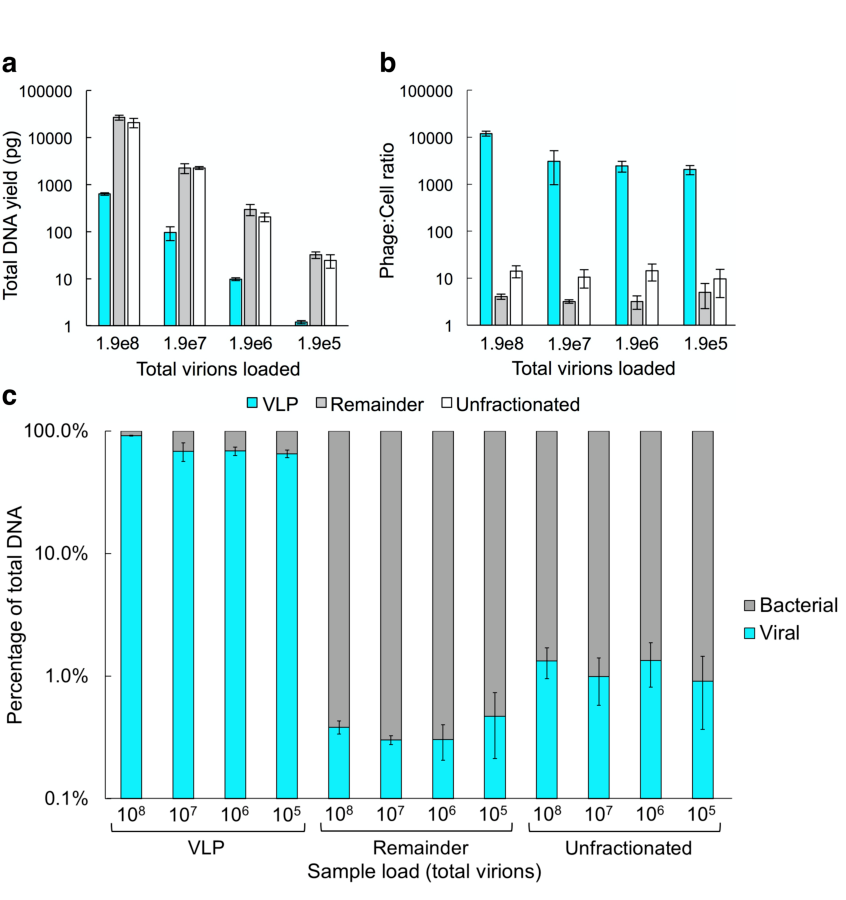
\includegraphics[width=\textwidth]{fig/C2fig3ABC.pdf}
\caption{Mass of DNA recovered from swabs loaded with different amounts of M13 and cells. Total (phage + bacterial) DNA mass recovered as determined by Qubit (a), recovered phage:cell ratio (B) and DNA composition by mass (C) in different fractions, as determined by qPCR. Negative controls for qPCR containing no template were not quantifiable after 40 cycles of PCR. Error bars indicate standard deviation among biological triplicates.}
\label{fig:dnarec}
\end{figure}
\end{subsection}

\begin{subsection}{Limit of detection of phage swabbed from human skin}
Having validated the method using phage:cell mixtures placed directly onto swabs, we moved to determine recovery of DNA when including the second potential source of loss, swabbing from human skin. An M13KO7 phage stock was serially diluted ten-fold and samples were loaded onto human skin, then swabbed immediately or allowed to dry prior to swabbing. Swabs were processed analogously to the above experiments. Near quantitative yield was obtained, for samples in which $\sim 10^{5}$ or more virions were loaded onto the skin (Figure \ref{fig:M13crv}). Lower sample loads than this could not be distinguished from qPCR background. Wet samples were observed to have consistently higher yields than dry samples; this phenomenon may be due to denaturation of phage upon drying and was also observed for T4, which showed a pronounced decrease in recovery for dried samples (see next section). The limit of detection of $\sim 10^{5}$ virions corresponds to $\sim 400$ fg of ssDNA.

\begin{figure}
\centering
\centerline{\includegraphics[width=\textwidth]{fig/C2fig4.pdf}}
\caption{Quantitative recovery of M13 loaded onto skin and then swabbed immediately (blue) or after drying (orange), as determined by qPCR. Expected or observed DNA copies per swab is indicated. Complete recovery is indicated by the dotted green line. A negative control (red) indicates experimental background determined by loading of 1X TE onto skin followed by swabbing and qPCR, and therefore reflects the combined background from skin, swabbing and extraction, and qPCR reagents. Error bars indicate standard deviation among biological triplicates.}
\label{fig:M13crv}
\end{figure}
\end{subsection}

\begin{subsection}{Recovery of T4 and bacterial DNA from skin swabs} %% this section is causing compilation errors!!!
To test the compatibility of other phage morphologies with this method, analogous experiments were performed using the canonical \textit{Caudovirales} phage T4, in place of M13K07, for a skin swabbing experiment. A $\Delta$\textit{ompC} $\Delta$\textit{ompF} strain of \textit{E. coli} was selected for this experiment to avoid the confounding effect of phage adsorption and infection. T4 and \textit{E. coli} were titered spectrophotometrically and mixed in a 10:1 ratio ($10^{8}$ virions:$10^{7}$ cells), loaded onto skin, then swabbed immediately while wet. DNA recovery values were comparable to the M13 experiment. In the remainder fraction, phage recovery $r_{p} = 0.32 \pm 0.03\; (y_{p} = 64\%)$ and bacterial recovery $r_{b} = 0.26 \pm 0.04\; (y_{b} = 26\%)$ were similar to unfractionated samples $(r_{p} = 0.53 \pm 0.12$ and $r_{b} = 0.34 \pm 0.08)$ (Figure \ref{fig:T4rec}a,b). In the VLP fraction, phage recovery $r_{p} = 0.27 \pm 0.03\; (y_{p} = 54\%)$ and bacterial recovery $r_{b} = 0.004 \pm 0.001$ ($y_{b}$ is undefined) indicated enrichment of phage, as expected. Controls in which phage and cells were applied directly to the swab showed similar recoveries, consistent with expectation given near quantitative yield from swabs.

Total phage DNA mass recovered is substantially higher than for M13KO7, consistent with the larger genome of T4, with the amount of DNA recovered from the VLP fraction being $5.1 \pm 0.6$ ng, and DNA recovery from the remainder fraction being $18 \pm 3$ ng on average. These amounts are more than sufficient for typical next-generation sequencing (NGS) preparation protocols.

The recovered DNA from the VLP fraction was composed of $96 \pm 1$\% T4 DNA by mass, a substantial increase compared to the unfractionated control $(32 \pm 2\%)$ (Figure \ref{fig:T4rec}c). This increase is less dramatic than for M13K07, due to the larger genome size of T4. Apparent phage:cell ratios after recovery also indicate significant viral enrichment, as fractionation resulted in a phage:cell
ratio of $\sim 700:1$ in the VLP fraction, compared to that of unfractionated controls $(\sim 17:1)$ (Figure \ref{fig:T4rec}d).

Swabbing was also performed from dried T4 samples, but these were found to produce very low yields in the VLP fraction compared to the analogous M13K07 experiment. However, the remainder fraction of the dried samples gave T4 DNA amounts comparable to swab controls, indicating that dried T4 could be recovered from the skin but was lost in the VLP purification process. We hypothesized that this was due to capsid damage that occurred during desiccation on the skin, which then exposed phage DNA to DNase digestion and thus reduced DNA purified in the VLP fraction. A plaque-forming assay was performed to determine the concentration of viable phage particles after desiccation; indeed, the VLP fraction from dried T4 produced $\sim$100-fold fewer plaques than the VLP fraction of a wet T4 sample.

\begin{figure}
\centering
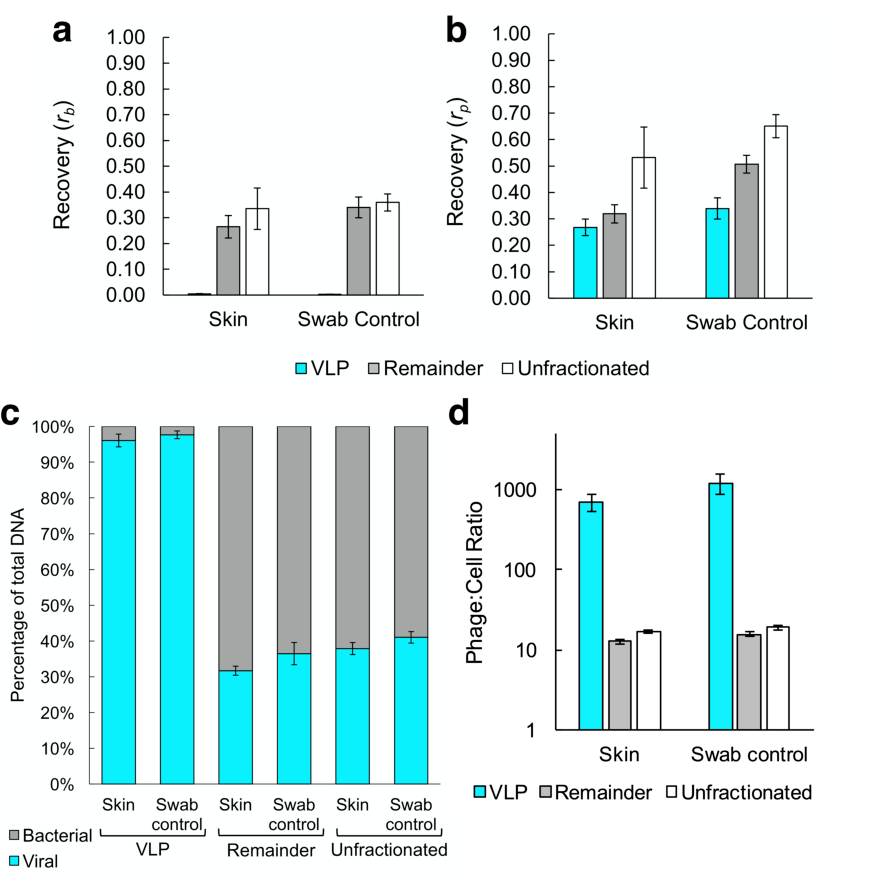
\includegraphics[width=\textwidth]{fig/C2fig5ABCD.pdf}
\caption{Recovery and mass yield from mock skin and swab samples with phage T4. Bacterial (A) and phage T4 (B) DNA recoveries were determined by qPCR for a single sample load (see Methods). $1.0 \times 10^{8}$ virions and $1.0 \times 10^{7}$ cells). Negative controls for qPCR containing no template were not quantifiable after 40 cycles of PCR. DNA composition (C) and phage:cell ratios (D) as determined by qPCR characterize T4 enrichment in the VLP fraction (same legend as A and B). Error bars indicate standard deviation among biological triplicates.}
\label{fig:T4rec}
\end{figure}
\end{subsection}

\begin{subsection}{Recovery of bacterial and phage DNA from clinical wound and skin swabs}
To test whether this processing method improved recovery of phage DNA from clinical swab samples, swabs were obtained from normal skin and wounds collected from patients at a wound clinic and processed in preparation for high throughput sequencing. We compared the novel sample preparation method (pilot study 2, or PS2) to a standard kit-based extraction method (pilot study 1, or PS1) by measuring dsDNA yields fluorometrically. Using PS1, only 10\% of skin VLP fractions and 25\% of wound VLP fractions yielded detectable DNA. However, PS2 gave significant improvement, producing detectable

DNA in 30\% of skin VLP samples and 100\% of wound VLP samples (Figure \ref{fig:yieldcomp}). Of VLP samples containing a detectable amount of DNA, PS2 yielded 6.7- and 4.4-fold greater average DNA concentration for skin and wound swabs, respectively, compared to PS1. Remainder fractions, which include substantial bacteria, are expected to contain more DNA, and as expected, nearly all skin and wound samples produced a detectable amount of DNA in the remainder fraction. In addition, PS2 gave 3.9- and 16.6-fold higher average DNA concentration compared to PS1, indicating that PS2 would also improve DNA yield for whole metagenome studies.

\begin{figure}
\centering
\includegraphics[width=\textwidth]{fig/C2fig6.pdf}
\caption{Comparison of DNA yields from clinical skin and wound swabs using kit-based extraction (PS1) and the method described here (PS2). DNA was quantified fluorometrically by Qubit assay. Limit of detection is indicated by the dashed line (LOD). for the Qubit dsDNA HS assay = \SI{10}{\pico\gram\per\micro\liter} according to supplier documentation \cite{RN85}). The fraction of samples above the LOD (n) is listed. All negative controls, which were exposed to air in the collection room or blank extractions, were below the LOD.}
\label{fig:yieldcomp}
\end{figure}

To assess the quality of the extracted DNA, samples from both studies were sequenced by paired-end Illumina MiSeq. Bacterial composition of the remainder fractions was determined by 16S rRNA sequencing using the V1-V3 loops (Figure \ref{fig:clinical}a). Both skin and wound samples from PS1 were largely dominated by \textit{Burkholderiaceae,} a well known kit contaminant \cite{RN70, RN71}. However, PS1 wound samples also contained low levels of previously reported skin colonizers such as \textit{Corynebacteriaceae, Staphylococcaceae,} and \textit{Pseudomonadaceae} \cite{RN72}. In contrast, PS2 skin and wound samples did not suffer from the same apparent kit contamination as PS1, and PS2 samples appear to contain archetypal skin and wound microbiomes. On average, the most abundant PS2 skin community members were commensals and opportunists, including \textit{Corynebacteriaceae, Staphylococcaceae, Proprionibacteriaceae,} and \textit{Micrococcaceae} \cite{RN72, RN73}. PS2 wound samples had high levels of \textit{Staphylococcaceae} and \textit{Enterobacteriaceae,} as well as lower levels of other previously reported wound colonizers like \textit{Bacteroidaceae, Campylobacteriaceae, Clostridiales, Porphyrmonadaceae, Pseudomonadaceae,} and \textit{Streptococcaceae} \cite{RN14, RN75, RN7}. These findings confirm that the novel fractionation and extraction protocol produces high quality DNA sufficient for sequencing, resulting in improved community recapitulation compared to the kit-based extraction used here. 

\begin{figure}
\centering
\includegraphics[width=0.6\textwidth]{fig/C2fig7AB.pdf}
\caption{Comparisons of DNA composition from clinical skin and wound swabs using kit-based extractions (PS1) and the method described here (PS2). For the remainder fraction, bacterial community composition was determined by 16S rRNA sequencing (a). Composition was summarized by averaging the relative abundance of taxa at the Family level across sample type (skin or wound). Families with $> 2$\% average relative abundance are shown. Recovery of viral DNA in the VLP-enriched fraction was estimated by shotgun sequencing and read mapping to the IMG/VR viral metagenome database (b). Percentage of reads mapped per sample are plotted here, and mean percentages are compared by $t$-tests.}
\label{fig:clinical}
\end{figure}

VLP-enriched samples were shotgun sequenced, and the quantity of recovered viral DNA was estimated by mapping quality-controlled reads to the Joint Genome Institute’s integrated microbial genomes viral analysis (IMG/VR) metagenomic database (Figure \ref{fig:clinical}b). On average, only $1.1 \pm 1.2\%$ of PS1 skin reads and $2.2 \pm 4.3\%$ of PS1 wound reads mapped to the database. PS2 samples had significantly higher viral mapping rates, with averages of $15.2 \pm 8.9\%$ for skin samples and $7.5 \pm 13.2\%$ for wound samples, which corresponded to higher absolute number of known viral reads (Figure \ref{fig:suppcomp}a). However, PS2 samples also had higher levels of human DNA contamination (Figure \ref{fig:suppcomp}b). Although the IMG/VR database is likely largely incomplete, these results show that the novel method produces more known viral reads on average.

\begin{figure}
\centering
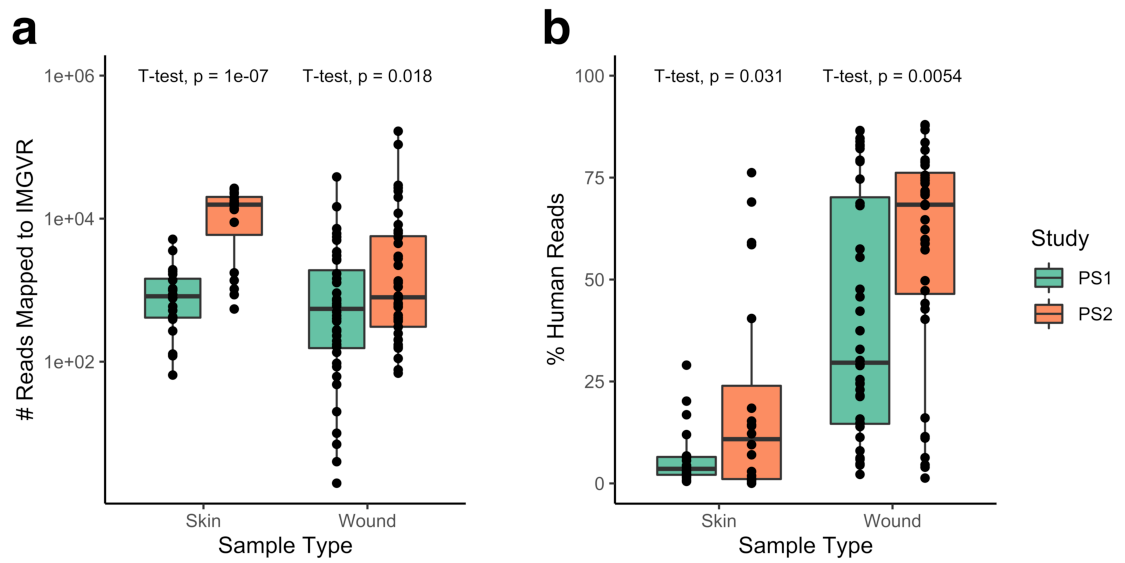
\includegraphics[width=\textwidth]{fig/C2figS2AB.pdf}
\caption{Comparisons of VLP-enriched DNA composition from clinical skin and wound swabs using kit-based extraction (PS1) and the method described here (PS2). VLP-enriched DNA was shotgun sequenced and mapped to the IMG/VR viral metagenome database (A) and the human genome (B). Means are compared by $t$-tests.}
\label{fig:suppcomp}
\end{figure}

\end{subsection}

\end{section}

%---  Discussion-------------------------
\begin{section}{Discussion}
As microbiome studies advance, there is increasing interest in the relatively understudied virome. However, experimental methodology for virome sampling has not been characterized and optimized as extensively as methods for bacterial sample processing. A central issue is the low biomass of phages in samples obtained from skin and wounds, which leads to insufficient material for sequencing or inadequate sequencing depth. Previously reported methods tend to be lengthy, not optimized for small volume, low-biomass samples, and/or do not retain the non-VLP fraction of the microbiome, requiring acquisition of a second sample for virome and whole
microbiome analysis. These factors limit practical usage in a clinical setting.

Here, we describe a streamlined method for preparing both viral-enriched and whole microbiome samples from a single, low-biomass skin or wound swab. Using this method, we produce VLP-enriched samples with several hundred-fold enrichment of viral DNA and also retain a whole microbiome fraction. Both fractions typically yield sufficient quantity of DNA for sequencing library preparation. This method may provide the following practical benefit in a clinical setting. In addition to only requiring one swab, in comparison to traditional methods (PS1), in which the majority of skin and wound VLP samples did not yield sufficient DNA for further analysis, the technical improvements presented here (PS2) produce sufficient VLP DNA from 100\% of wound swabs and 30\% of skin swabs. The increased yield from this protocol is likely due to the accumulation of small improvements. For example, buffer concentrations were chosen to facilitate replicable pipetting and reduce total sample volume, allowing precipitation and extraction steps to be performed in microcentrifuge tubes and a single phase-lock gel tube, thus minimizing loss from transfers. Additionally, we find that the use of ethanol precipitation for VLP DNA purification is more efficient than column- based purification. Most of the buffers are not available off-the-shelf in the concentrations used here, but are easily prepared and stored as such. The PS2 workup requires more time at the bench, but is less costly in terms of reagents in addition to consistently producing higher DNA yields than PS1, in turn producing higher quality 16S rRNA and metagenomic sequencing data.

This protocol was developed with the goal of capturing free ssDNA and dsDNA phages, so mock specimens were chosen accordingly to characterize the protocol (M13 and T4, respectively). These phages also represent a number of clinically important phages. As a member of \textit{Inoviridae}, M13 is a relative of the clinically implicated \textit{Pseudomonas aeruginosa} phage Pf \cite{RN77}. T4 is a member of the canonical dsDNA \textit{Caudovirales} family, which have previously been shown to be prominent members of the healthy skin virome \cite{RN56}. We noted that T4 survived poorly on the dessicated environment of the skin compared to M13; this may or may not be relevant depending on whether a study is intended to survey the viable phages. However, an important caveat of the present work is that the procedure is not optimized for lipid-encapsulated or RNA viruses. Additionally, in mock samples, phage:cell stock solutions were only prepared in an approximately 10:1 ratio, and variations of this ratio were not tested. Nevertheless, the clinical samples presumably varied in phage:cell ratio and other factors.

Although only a small proportion (typically $<1$\%) of the total bacterial DNA was found in the VLP fraction, the large molecular weight of bacterial DNA translates into a large mass fraction relative to phage DNA. This effect is pronounced in the case of M13, a very small phage ($\sim$ 8 kb ssDNA), for which $\sim$ 70\% of the VLP fraction consisted of phage DNA. We anticipate that $\sim$ 70\% thus represents a lower bound on the mass fraction of phage DNA in realistic settings where multiple viral species are recovered. As expected, the effect is less notice- able in the case of T4 ($\sim$123 kb dsDNA). Thus, despite the lack of lengthy purification steps (e.g., CsCl gradient centrifugation), most reads from a sequencing run using the VLP DNA would be expected to derive from phages.

We applied this method in the clinic and found that it dramatically reduced the amount of reagent and consumable contaminants detected in 16S rRNA sequencing data. Additionally, the method produced VLP-enriched samples with higher viral read mapping rates than the kit-based extractions. However, the viral read mapping rates were still relatively low, which is likely due to high human DNA contamination and an incomplete viral reference database. We hypothesize that the high level of human DNA contamination was due to increased DNA yields and insufficient DNase I digestion, which can be remedied with higher nuclease concentrations and increased incubation times. While IMG/VR is the most comprehensive viral metagenome database available \cite{RN78}, database matching is insensitive to novel viruses, which could account for a large proportion of the DNA; it is estimated that only 10–60\% of viral metagenomes align to reference databases \cite{RN79, RN80}. Use of this protocol could have several benefits for virome and microbiome studies, including increased patient recruitment due to minimal swabbing, improved experimental design using paired VLP and remainder fractions, reduced failure rate of DNA extraction from individual swabs, and improved detection of low abundance phages.

\end{section}

%---  Conclusion-------------------------
\begin{section}{Conclusion}
With rapid advancements in microbiome studies, the frequently overlooked virome is gaining interest. However, investigation of healthy and diseased human viromes from whole metagenome samples can be hindered by low-biomass samples. To overcome these challenges, VLP purification methods have been developed. However, previously reported methods are not compatible with small volume, low-biomass samples and do not retain the non-VLP fraction of the microbiome, requiring separate samples for virome and whole microbiome analysis. Here, we describe a method for preparing both viral-enriched and whole microbiome samples from a single, low-biomass skin swab to facilitate the study of viromes and microbiomes in dermatological diseases. Using this method, we produce VLP-enriched samples composed of $> 70$\% viral gDNA with up to 80\% yield of viral gDNA and less than 1\% yield of bacterial gDNA. The remaining whole microbiome fraction is retained in this process, allowing paired VLP and whole metagenome sequencing. In a clinical setting, this method improves both microbial community analysis as well as the number of viral reads, demonstrating that technical improvements can significantly impact the quality of sequencing data from low-biomass samples.
\end{section}

%---  Methods-------------------------
\begin{section}{Methods}
\begin{subsection}{Phage and bacterial sample preparation}
Mock samples were composed of M13KO7 phage and BL21(DE3) \textit{E. coli} (NEB C2527), or T4 phage and KJ740 \textit{E. coli} (CGSC 12151). The virion density of phage stocks was determined spectrophotometrically as follows. Absorbance was measured at \SI{269}{\nano\meter} and \SI{320}{\nano\meter} and converted to virions/\si{\milli\liter} by the following equation: virions/\si{\milli\liter} = $[(A269 nm - A320 nm) \times (6 \times 1016)]$/genome length (8669 bp for M13KO7, 168.903 kb for T4). 5 mL cultures of \textit{E. coli} were inoculated by a single colony and grown in Luria broth (LB) overnight in the presence of $\SI{100}{\micro\gram\per\mL}$ ampicillin for strain BL21(DE3) or $\SI{10}{\micro\gram\per\mL}$ tetracycline for strain KJ740. Cell density of \textit{E. coli} overnight cultures was measured by optical density at 600 nm (OD600) with 4- and 10-fold dilutions, and converted to cells/mL using a conversion factor of $3.2 \times 10^{8}$ cells/mL per OD600 unit. This conversion factor was experimentally determined by comparing OD600 measurements and colony-forming unit (CFU) counts of overnight cultures. Known concentrations were used to create a mixed phage and cell stock solution in a 19:1 ratio, for final concentrations of $9.5 \times 10^{6}$ virions/$\si{\micro\liter}$ and $5.0 \times 10^{5}$ cells/$\si{\micro\liter}$, in 0.5X TE, 0.5X LB (phage stock was diluted in 1X TE and cells were diluted in LB). For M13KO7 viral enrichment experiments, the mixed stock was 10-fold serially diluted 3 times in LB to create a sample range of $9.5 \times 10^{5} – 9.5 \times 10^{3}$ virions/$\si{\micro\liter}$ ($5.0 \times 10^{4} – 1.0 \times 10^{2}$ CFU/$\si{\micro\liter}$), and $\SI{20}{\micro\liter}$ of each dilution was loaded directly onto a sterile swab. In the T4 viral enrichment experiment, one mixed stock was created at $5.0 \times 10^{6}$ virions/$\si{\micro\liter}$ ($5.0 \times 10^{5}$ CFU/$\si{\micro\liter}$).
\end{subsection}

\begin{subsection}{Swabbing from human skin}
All swab experiments were performed with sterile Copan FLOQSwabs 520C. Three healthy volunteers were enrolled after obtaining informed consent according to procedures approved by the UCSB Human Subjects Committee and Institutional Review Board (Protocol 4-18-0190 and 2-18-0059). M13KO7 phage alone was diluted serially in 1X sterile TE, for a concentration range from $1.9 \times 10^{8}$ to $1.9 \times 10^{2}$ virions/$\si{\micro\liter}$. For skin sampling experiments, skin on the left forearm of the volunteer was wiped with 70\% ethanol. Then, sample was applied to the skin (\SI{20}{\micro\liter} for T4 experiments or \SI{10} {\micro\liter} for M13K07 experiments), covering an area of approximately \SI{0.25}{\centi\meter\squared}, and either swabbed immediately or allowed to dry for 30 minutes. The swab was pre-wetted with sterile 1X TE and then rotated 10 times over a $\sim$ \SI{1}{\centi\meter\squared} area (length of the swab tip = \SI{1}{\centi\meter\squared}) with gentle pressure (Levine’s technique). The yield of phages and bacteria recovered from such a swab reflects two steps: gathering of material from the skin, and release of material from the swab. To separately quantify the yield of phage and cells released from the swab, the same volume of the stock dilution series was applied directly to a different swab. Swabs containing sample were processed further within 30 minutes. Negative controls were performed by pipetting an equal volume of 1X TE onto the skin and following the procedure outlined above.
\end{subsection}

\begin{subsection}{Fractionation of virus-like particles (VLPs)}
After swabbing, the swab tip was inserted into a \SI{1.5}{\milli\liter} microcentrifuge tube and snapped at the \SI{30}{\milli\meter} break-point. \SI{500}{\micro\liter} of sterile 1X TE was added to the tube, and the tube was vortexed for 2 minutes at maximum speed on a multitube vortex adapter to resuspend the sample. Samples were then centrifuged at $16,000 \times g$ for 2 minutes to pellet cells. \SI{250}{\micro\liter} of supernatant was transferred to a \SI{2}{\mL} microcentrifuge tube for immediate VLP precipitation (the VLP fraction). The remaining \SI{250}{\micro\liter} of supernatant, pelleted cells, and swab tip (the ‘remainder’ fraction) were kept in the original tube and stored at \SI{-20}{\celsius} before proceeding to DNA extraction.
\end{subsection}

\begin{subsection}{Isolation of DNA from virus-like particles}
To digest free DNA in the VLP fraction, \SI{2}{\micro\liter} of 126X DNase I reaction buffer (\SI{441}{\milli\molar} MgCl\textsubscript{2}, \SI{63}{\milli\molar} CaCl\textsubscript{2}) and \SI{2.5}{\micro\liter} DNase I (5 units, NEB) were added to the VLP fraction, mixed by inversion, and incubated at \SI{37}{\celsius} for 30 minutes. DNase I was inactivated by incubation at \SI{75}{\celsius} for 10 minutes. VLPs were precipitated by adding \SI{25}{\micro\liter} sterile 1X TE (pH 8.0), \SI{2.5}{\micro\liter} \SI{0.5}{\molar} EDTA (pH 8.0), \SI{250}{\micro\liter} formamide, \SI{7}{\micro\liter} glycoblue (\SI{15}{\milli\gram\per\mL}), and \SI{1.1}{\mL} 100\% ethanol, followed by incubation at \SI{-20}{\celsius} for 1 hour and centrifugation for 1 hour at $> 10,000 \times g$ at \SI{4}{\celsius}. Pellets were washed with \SI{500}{\micro\liter} of ice cold 70\% ethanol and re-pelleted by centrifugation for 30 minutes at $> 10,000 \times g$ at \SI{4}{\celsius}. Pellets were dried for 1 hour at room temperature in a vacufuge before being resuspended in \SI{152}{\micro\liter} sterile 1X TE (pH 8.0).

Viral capsids were disrupted and digested by adding \SI{19.6}{\micro\liter} of 10\% SDS and \SI{21.4}{\micro\liter} proteinase K (\SI{20}{\milli\gram\per\mL}) to the resuspended VLPs, followed by incubation at \SI{55}{\celsius} for 1 hour. Then, \SI{32}{\micro\liter} of \SI{5}{\molar} NaCl and \SI{25}{\micro\liter} CTAB-NaCl were added followed by incubation at \SI{65}{\celsius} for 10 minutes. The \SI{250}{\micro\liter} sample was then transferred to a phase lock gel tube (5PRIME PLG Light) and mixed with \SI{250}{\micro\liter} of 25:24:1 phenol:chloroform:isoamyl alcohol by inversion. Phases were separated by centrifugation at $1500 \times g$ for 5 minutes. In the same tube, 24:1 chloroform: isoamyl alcohol extraction was performed twice and centrifuged as described above, and the \SI{250}{\micro\liter} aqueous phase was transferred to a \SI{2}{\mL} microfuge tube. DNA was precipitated by adding \SI{27.5}{\micro\liter} of \SI{3}{\molar} sodium acetate (pH 5.2), \SI{1}{\micro\liter} Glycoblue (\SI{15}{\milli\gram\per\mL}), and \SI{1.5}{\mL} 100\% ethanol followed by incubation at \SI{-80}{\celsius} for 1 hour and centrifugation at $> 13,000 \times g$ at \SI{4}{\celsius}. Pellets containing DNA were washed with \SI{500}{\micro\liter} ice cold 70\% ethanol, centrifuged at $> 13,000 \times g$ at \SI{4}{\celsius} for 30 minutes, dried for 1 hour at room temperature in a vacufuge, and resuspended in \SI{20}{\micro\liter} 1X TE (pH 8.0).
\end{subsection}

\begin{subsection}{Extraction of genomic DNA from the remainder fraction and unfractionated samples}
Samples were thawed on ice, then vortexed for 2 minutes at maximum speed using a multitube vortex adapter to resuspend the cells. Keeping the swab in the tube, lysis was performed by adding \SI{5}{\micro\liter} of \SI{5}{\molar} NaCl and \SI{45}{\micro\liter} of Ready-Lyse lysozyme (250 U/\si{\micro\liter}) (Epicentre), followed by incubation at room temperature for 30 minutes. Lysis continued with addition of \SI{33}{\micro\liter} of proteinase K (\SI{20}{\milli\gram\per\mL}) and \SI{333}{\micro\liter} of PureLink Genomic Lysis/Binding buffer (Thermo), followed by incubation at \SI{55}{\celsius} for 1 hour. Physical lysis was conducted with bead beating by adding \SI{2}{\gram} of \SI{0.5}{\milli\meter} glass beads to the sample and vortexing at maximum speed for 10 minutes using a multitube vortex adapter. \SI{333}{\micro\liter} of 100\% ethanol was added to the sample and mixed by inversion, and the entire sample was loaded onto a PureLink Genomic DNA Mini Kit column (Thermo). DNA cleanup and elution was performed using the kit’s guidelines, with an elution volume of \SI{25}{\micro\liter} EB.
\end{subsection}

\begin{subsection}{Collection, processing, and quantification of clinical samples}
Clinical sample collection was performed at Ridley-Tree Center for Wound Management at Goleta Valley Cottage Hospital in accordance with protocols approved by the Cottage Health Institutional Review Board (Study Protocol 16-52u and 17-48u). We recruited a cohort of 40 wound care patients and collected samples after obtaining informed consent from the patient. Exclusion criteria were: patients under the age of 18, in the intensive care unit, or presenting with an unrelated non-wound infection. Four clinically classified chronic wound types were sampled (diabetic, venous, arterial, and pressure ulcers), with ten patients per wound type. Wound swabs were collected pre- and post-debridement, and a healthy skin swab was collected from the contralateral limb. Negative control samples were collected by exposing swabs to air in the collection room for the same duration as wound and skin swab collection. All swabs were collected using Levine’s technique as described above for the mock samples. Swabs were placed back into the dry, sterile collection tube and stored at \SI{4}{\celsius} for no more than four hours before being processed.

To determine whether the fractionation and purification procedures described above affected DNA yield from swabs obtained in a clinical setting, samples from 20 patients (five patients per wound type; designated as PS1 samples) were processed using a standard processing protocol, while samples from the other 20 patients (five patients per wound type; designated as PS2 samples) were processed using the fractionation and extraction methods described in detail above. The standard processing protocol for PS1 is as follows: \SI{500}{\micro\liter} of sterile 1X TE was added to the collection tube and vortexed for 2 minutes at maximum speed to resuspend the sample, which was then transferred to a microcentrifuge tube and centrifuged at $16,000 \times g$ to pellet cells, then \SI{250}{\micro\liter} of supernatant was filtered using a \SI{13}{\milli\meter} diameter \SI{0.45}{\micro\meter} polyethersulfone syringe filter to produce the VLP fraction while the remaining \SI{250}{\micro\liter} supernatant and pellet constituted the remainder fraction. VLP fractions were subjected to DNase I treatment as described above, then extracted using the PureLink Viral RNA/ DNA Mini Kit following the manufacturer’s instructions with an elution volume of \SI{25}{\micro\liter}. The remainder fraction was extracted using the PureLink Genomic DNA Mini Kit following the manufacturers instructions with an elution volume of \SI{25}{\micro\liter}. DNA yields were quantified fluorometrically using the Qubit dsDNA High Sensitivity kit on the Qubit 3 instrument, with \SI{5}{\micro\liter} of sample used per assay.
\end{subsection}

\begin{subsection}{Quantitative PCR}
To generate stocks for qPCR standard curves, M13KO7 and T4 virion DNA was extracted using the PureLink Viral RNA/DNA Mini Kit and \textit{E. coli} gDNA was purified using the PureLink Genomic Mini Kit. Stock concentrations were determined by Qubit ssDNA and dsDNA High Sensitivity reagents. Stocks were then diluted in sterile 1X TE to create 10-fold dilution series with the following concentration ranges: $1.8 \times 10^{9}$ to 18 copies/\si{\micro\liter} for M13K07; $1.7 \times 10^{7}$ to 17 copies/\si{\micro\liter} for T4; $1.1 \times 10^{6}$ to 11 copies/\si{\micro\liter} for BL21(DE3) \textit{E. coli}; $1.3 \times 10^{7}$ to 13 copies/\si{\micro\liter} of KJ740 \textit{E. coli}. qPCR primers were designed on Benchling using Primer3 and were purchased from Integrated DNA Technologies, generating 100 bp amplicons for M13, T4, and the 16S rDNA V1 loop of \textit{E. coli}. Primer sequences used: 
\begin{itemize}
\item M13K07
	\begin{itemize}
		\item Forward: $5^{\prime}$-TCTGTACACCGTTCATCTGTCC-$3^{\prime}$ 
		\item Reverse: $5^{\prime}$-ACCTGCTCCATGTTACTTAGCC-$3^{\prime}$ 
	\end{itemize}
\item T4 
	\begin{itemize}
		\item Forward: $5^{\prime}$-AGCGACCCGGTTTCTCATTT-$3^{\prime}$
		\item Reverse: $5^{\prime}$-AAATTACGTCCCGCTGGTGT-$3^{\prime}$
	\end{itemize}
\item 16S rDNA V1 loop 
	\begin{itemize}
		\item Forward: $5^{\prime}$-ATTGAACGCTGGCGGCAGG-$3^{\prime}$ 
		\item Reverse: $5^{\prime}$-CCCAGACATTACTCACCCGTCCG-$3^{\prime}$
	\end{itemize}
\end{itemize}
qPCR experiments were performed using Bio-Rad SsoAdvanced Universal SYBR Green Supermix and Bio-Rad CFX96 thermal cycler with CFX96 Real-Time PCR Detection System. Final volume of the reaction was \SI{20}{\micro\liter}, containing \SI{10}{\micro\liter} of SYBR Green Supermix, \SI{1}{\micro\liter} of each primer at \SI{10}{\micro\molar}, \SI{1}{\micro\liter} template, and \SI{7}{\micro\liter} of PCR-grade water. 40 cycles of PCR were performed, followed by melting curve analysis. Concentration data were converted to mass using genomic molecular weights determined using the following approximations: molecular weight (MW) of ssDNA genome = genome length (bases) $\times \SI{303.7}{\gram\per\mole} + \SI{79}{\gram\per\mole}$; MW of dsDNA genome = genome length (base pairs) $\times \SI{607.4}{\gram\per\mole} + \SI{157.9}{\gram\per\mole}$.
\end{subsection}

\begin{subsection}{16S rRNA library preparation, sequencing, and bioinformatics}
16S sequencing libraries were generated by two-step PCR for each sample. In the first step, V1-V3 loops were amplified using custom adapter primers composed of universal 16S primers ‘27F’ and ‘534R’ and Illumina Nextera indexing adapter sequences. Adapter PCR was done in \SI{25}{\micro\liter} reactions containing \SI{11.5}{\micro\liter} of template, \SI{0.5}{\micro\liter} of each primer at \SI{10}{\micro\molar}, and \SI{12.5}{\micro\liter} of KAPA HiFi HotStart ReadyMix. 25 cycles of PCR were performed under the following conditions: denaturation at \SI{95}{\celsius} for 30 seconds, annealing at \SI{55}{\celsius} for 30 seconds, and extension at \SI{72}{\celsius} for 30 seconds. PCR products were purified with \SI{20}{\micro\liter} AMPureXP beads and eluted into \SI{50}{\micro\liter} of \SI{10}{\milli\molar} Tris pH 8.5. In the second step, Illumina Nextera XT indices were added by PCR in \SI{50}{\micro\liter} reactions containing \SI{5}{\micro\liter} of product from adapter PCR, \SI{5}{\micro\liter} of Index 1, \SI{5}{\micro\liter} of Index 2, \SI{25}{\micro\liter} of KAPA HiFi HotStart ReadyMix, and \SI{10}{\micro\liter} of water. 8 cycles of PCR were conducted under the same conditions as step 1. Indexed samples were purified with \SI{56}{\micro\liter} of AMPureXP beads, eluted into \SI{25}{\micro\liter} of \SI{10}{\milli\molar} Tris pH 8.5, quantified with a Qubit dsDNA HS kit, normalized and pooled for multiplexing. Final library QC was done using an Agilent TapeStation dsDNA 1000 bp kit. The final libraries were sequenced on an Illumina MiSeq with PE300 V3 chemistry at UCSB’s Biological Nanostructures Laboratory (BNL) sequencing core.

Paired-end reads were uploaded to the Quantitative Insights Into Microbial Ecology Amazon Web Services Amazon Machine Image (QIIME AWS AMI) (AMI ID: ami-1918ff72, “qiime-191”) \cite{RN81}. Initial quality analysis was performed with FastQC. Reads were quality controlled by trimming and quality filtering with trimmomatic using default settings \cite{RN82}. Read joining was performed with QIIME’s joining script (join\_paired\_ends.py), using the fastq-join algorithm with default settings. Joined reads were fed into the open operational taxonomic unit (OTU) picking pipeline (pick\_open\_reference\_otus.py) using default settings. Taxonomy was assigned using the SILVA128 16S reference database clustered at the 97\% identity threshold \cite{RN35}. The final Biological Observation Matrix (BIOM) table (without PyNAST alignment failures) and metadata mapping files were imported into RStudio using the phyloseq package for downstream analyses \cite{RN45}. Samples were sorted from controls, taxonomy was summarized by agglomerating at the family level, and absolute OTU abundance was converted to relative abundance per sample and averaged within sample type (skin vs. wound) within each study (PS1 and PS2). PS1 and PS2 phyloseq objects were converted to table format and filtered to remove any taxa with relative abundance less than 2\%, and plotted with ggplot2 [38].
\end{subsection}

\begin{subsection}{VLP-enriched library preparation, sequencing, and bioinformatics}
DNA from VLP-enriched samples was amplified by random hexamer-primed multiple strand displacement amplification (GenomiPhi V3, GE Healthcare), following the manufacturer’s protocol. Amplified DNA was purified with \SI{40}{\micro\liter} of AMPureXP beads and eluted into \SI{15}{\micro\liter} of \SI{10}{\milli\molar} Tris pH 8.5. Amplified samples were normalized to \SI{0.2}{\nano\gram\per\micro\liter} and prepared for shotgun sequencing with the Nextera XT kit and Nextera XT indices, as described by the manufacturer. Indexed samples were quantified with a Qubit dsDNA HS kit, normalized, and pooled. Final library QC was done using Agilent TapeStation dsDNA 5000 bp and 1000 bp kits. Final libraries were sequenced on an Illumina MiSeq with PE150 (PS1) or PE300 (PS2) chemistry, at the UC Davis Genome Center.

Paired-end reads were uploaded to a custom AWS AMI (AMI ID: ami-19acbf62, “Chen Lab VMM Basic Image 1.1”) for bioinformatic processing. Initial quality analysis was performed with FastQC. Reads were quality controlled by trimming and quality filtering with trimmomatic using default settings \cite{RN82}. All read mapping steps were performed with Bowtie2 using the –sensitive and –non-deterministic settings, with mapping summaries printed to file \cite{RN85}. Reads were first mapped to the human genome (GRCh38.p13, NCBI accession: GCF\_000001405.39). Reads that did not map to the human genome were collected and known viral lab contaminants were removed by mapping to M13 and fd genomes. Remaining reads were mapped to the Joint Genome Institute’s IMG/VR database (IMG\_VR\_2018-07-01\_4) \cite{RN78}, currently the largest public database of viral metagenomes. Overall alignment rates were extracted from the mapping summaries, assembled into tables, imported to RStudio, and plotted with ggplot2 \cite{RN46}. T-tests were performed with ggpubr.
\end{subsection}


\end{section}

%=== Chapter 3  ============================================
\chapter{Microbial predictors of healing and short-term effect of debridement on the microbiome of chronic wounds: the role of facultative anaerobes}\newpage
\label{Chapter 3}

%---  Abstract -------------------------
\begin{section}{Abstract}
Chronic wounds represent a large and growing disease burden. Infection and biofilm formation are two of the leading impediments of wound healing, suggesting an important role for the microbiome of these wounds. Debridement is a common and effective treatment for chronic wounds. We analyzed the bacterial content of the wound surface from 20 outpatients with chronic wounds before and immediately after debridement, as well as healthy skin. Given the large variation observed among different wounds, we introduce a Bayesian statistical method that models patient-to-patient variability and identify several genera that were significantly enriched in wounds vs. healthy skin. We found no difference between the microbiome of the original wound surface and that exposed by a single episode of sharp debridement, suggesting that this debridement did not directly alter the wound microbiome. However, we found that aerobes and especially facultative anaerobes were significantly associated with wounds that did not heal within 6 months. The facultative anaerobic genus \textit{Enterobacter} was significantly associated with lack of healing. The results suggest that an abundance of facultative anaerobes is a negative prognostic factor in the chronic wound microbiome, possibly due to the increased robustness of such communities to different metabolic environments.
\end{section}

%---  Introduction -------------------------
\begin{section}{Introduction}
Chronic wounds are wounds that fail to exhibit reasonable healing progress within an expected time frame (e.g., three to six weeks) \cite{RN2, RN3}. It is estimated that in the U.S. alone, over 6.5 million people are affected, costing the healthcare system at least \$25 billion annually \cite{RN4}. Although the burden of chronic wounds is often overlooked or obscured by overall burden of the primary disease \cite{RN2, RN3}, these wounds have a notable impact on quality of life, reducing mobility and inducing chronic pain. Older patients with established diseases, particularly diabetes, obesity, venous insufficiency, peripheral artery disease, and immobility, are at highest risk of developing chronic wounds \cite{RN4}. As these risk factors increase in prevalence, the economic and human costs of chronic wounds are expected to grow.

One of the leading impediments to healing of chronic wounds is infection and associated pathological inflammation \cite{RN5}. Although chronic wounds are not always infected, they may be colonized by a distinct microbiome that could lead to infection or impact wound healing. While traditional, culture-dependent studies are now acknowledged to be unable to provide an extended view of diversity, more recent culture-independent studies over the past decade have established that wounds harbour diverse microbiota, with the primary constituents being \textit{Staphylococcus spp., Pseudomonas spp., Corynebacterium spp., Streptococcus spp., Anaerococcus spp.,} and \textit{Enterococcus spp.,} along with numerous low-abundance taxa \cite{RN6, RN7, RN8}. While chronic wounds are polymicrobial, they have lower diversity than healthy skin \cite{RN9}. Substantial inter-patient variability exists in the microbiome, which cannot be explained by age, race, sex, or wound etiology \cite{RN6, RN10}, and therefore statistical models that can account for inter-patient variability are desirable for modeling the chronic wound microbiome. Despite significant past work \cite{RN6, RN7, RN8, RN9, RN10, RN11, RN12, RN13, RN14, RN15, RN16, RN17, RN18, RN19, RN20, RN21, RN22, RN23, RN24, RN25, RN26, RN27, RN28}, additional studies on the wound microbiome are needed to understand its contribution, if any, to the pathophysiology of chronic wounds. Here we investigate how a single episode of sharp debridement affects the wound microbiome, as well as which constituents of the wound microbiome might correlate with healing.

A second leading impediment to wound healing is biofilm formation \cite{RN5, RN29}. One of the most common and widely effective chronic wound treatments is debridement, a standard-of-care procedure whose goal is physical disruption and removal of biofilms and necrotic or devitalized tissue \cite{RN30, RN31}. Besides stimulating reepithelialization and cell migration, debridement can reduce microbial load \cite{RN30, RN31}. However, relatively little is known about how debridement influences the composition of the microbial community of the wound. Previous work has found that microbiota isolated from debrided tissue and wound swabs are similar though not an exact match \cite{RN9}. A recent longitudinal diabetic foot ulcer study found that, after 2 weeks, debridement had significantly decreased the relative abundance of anaerobes, but only in the wounds that healed within 12 weeks \cite{RN8}. To determine whether this response occurred immediately vs. developed over the 2 week interval, we swabbed chronic wounds immediately after sharp debridement in the same clinic visit and compared the microbial communities before and after debridement, including a comparison of the abundance of individual taxa. 

An important focus of study for the chronic wound microbiome is the identification of correlations of the microbiome to healing outcomes. For example, Loesche et al. determined that temporal instability of communities, particularly the transition between several distinct community types, is associated with positive healing outcomes \cite{RN7}. Understanding which organisms are beneficial or detrimental could be important for evaluating prognosis or probiotic interventions. However, no specific taxa or metabolic types have yet been reported to be predictive of healing outcomes. We studied whether the presence of taxa with different oxygen requirements (aerobes, anaerobes, facultative anaerobes) or specific taxa predicted healing outcomes 6 months after wound sampling. 

In the present study, wound swabs were obtained from 20 patients presenting at a wound clinic, with 5 patients from each of four common chronic wound etiologies (diabetic, venous, arterial, and pressure ulcers). Swab samples were collected from chronic wounds before and after a single, sharp debridement event, along with a skin swab sample from a control site (e.g., the contralateral limb). Microbial communities were characterized by Illumina sequencing of the V1-V3 loops of 16S rRNA genes. Data were analyzed by ecological diversity metrics and differential abundance analysis with DESeq2 \cite{RN32}, a popular differential abundance method, and a Bayesian generalized linear mixed regression model (BGLMM) with patient-specific factors to account for inter-patient variabilities \cite{RN33}. Our analysis of debridement indicates that the newly exposed wound surface has minimal microbial difference from the old wound surface, and we identify bacterial taxa associated with healing outcomes. The implications of these findings on our understanding of the pathophysiology of chronic wounds is discussed.
\end{section}

%---  Results-------------------------
\begin{section}{Results}

\begin{subsection}{Bacterial composition of skin and chronic wound microbiomes}
Patient and wound characteristics are summarized in Table \ref{Tab:woundsummary}. A total of 18,128,419 paired-end sequencing reads were obtained from Illumina sequencing, with 14,025,888 reads assigned in demultiplexing. On average, there were 203,273 reads in each sample (minimum = 15,476 reads, maximum = 729,495 reads, median = 172,250 reads). Quality control analysis indicated sufficient sampling of the microbiome in all but one sample, which was excluded from analysis (Figure \ref{fig:S1AD}). 

% table 1 (wound summary table)
\begin{table}[h]
\caption{Patient and wound characteristics}
\label{Tab:woundsummary}
\adjustbox{max width=\textwidth}{%
\centering
\footnotesize
\begin{tabular}{llllllll}
\hline
\thead{Patient\\\#} & \thead{Wound\\type} & \thead{Healing\\outcome} & \thead{Wound size\\(\si{\centi\meter\squared})} & \thead{Level of\\debridement} & Instrument & \thead{\# previous\\debridements} & \thead{Days since\\last\\debridement}\\
\hline
1          & Diabetic   & Healed          & 1                   & Dermis               & Curette       & 0                         & 0                            \\
2          & Diabetic   & Unhealed        & 0.5                 & Dermis               & Curette       & 12                        & 14                           \\
3          & Diabetic   & Healed          & 3.57                & Dermis               & Curette       & 5                         & 8                            \\
4          & Diabetic   & Unhealed        & 68.7                & Subcutaneous         & Curette       & 6                         & 7                            \\
5          & Diabetic   & Unhealed        & 3.6                 & Subcutaneous         & Curette       & 7                         & 10                           \\
6          & Venous     & Unhealed        & 2.07                & Dermis               & Curette       & 33                        & 7                            \\
7          & Venous     & Unhealed        & 30                  & Dermis               & Curette       & 1                         & 7                            \\
8          & Venous     & Healed          & 11.6                & Dermis               & Curette       & 4                         & 9                            \\
9          & Venous     & Healed          & 445                 & Dermis               & Curette       & 2                         & 7                            \\
10         & Venous     & Healed          & 10                  & Subcutaneous         & Curette       & 3                         & 9                            \\
11         & Arterial   & Healed          & 0.2                 & Dermis               & Curette       & 6                         & 9                            \\
12         & Arterial   & Unhealed        & 307.84              & Dermis               & Curette       & 18                        & 7                            \\
13         & Arterial   & Unhealed        & 5.92                & Dermis               & Curette       & 13                        & 7                            \\
14         & Arterial   & Healed          & 6.4                 & Subcutaneous         & Curette       & 13                        & 7                            \\
15         & Arterial   & Unhealed        & 10.85               & Dermis               & Curette       & 2                         & 7                            \\
16         & Pressure   & Healed          & 0.2                 & Subcutaneous         & Tissue Nipper & 3                         & 12                           \\
17         & Pressure   & Unhealed        & 8.88                & Dermis               & Curette       & 20                        & 7                            \\
18         & Pressure   & Healed          & 0.9                 & Dermis               & Curette       & 19                        & 6                            \\
19         & Pressure   & Unhealed        & 4.62                & Subcutaneous         & Scalpel       & 4                         & 7                            \\
20         & Pressure   & Unhealed        & 1.35                & Dermis               & Curette       & 3                         & 7   \\
\hline                        
\end{tabular}}
\end{table}

We first verified that our results on the skin and wound microbiomes of the patients were consistent with previous findings \cite{RN8, RN21}. Sequenced 16S rRNA genes were clustered into operational taxonomic units (OTUs) using the open OTU picking method in QIIME \cite{RN81}, with taxonomy assigned using the SILVA128 database \cite{RN35} (see Figure \ref{fig:S1AD} for quality metrics). The accuracy of microbial community recapitulation was confirmed by analysis of a cell-based mock community. All expected members of the mock community were detected, but some deviations from the expected composition were observed (Figure \ref{fig:S2AB}a). In particular, a relative decrease of Gram-positive organisms compared to Gram-negative organisms suggests that incomplete lysis may cause relative under-representation of Gram-positive organisms in the samples. Negative control samples were analyzed to identify potential contaminants (Table \ref{Tab:negconotus}). Compositional data was obtained (i.e., relative abundance within each sample) and absolute abundance was not measured specifically. However, we noted that the absolute concentration of DNA extracted from negative control samples was undetectable by a Qubit assay but that nearly all skin and wound samples (59/60) resulted in detectable DNA \cite{RN41}, indicating that absolute abundances are generally higher in skin and wound samples compared to the negative controls. The four most abundant phyla detected on average across both skin and wound samples were \textit{Firmicutes, Proteobacteria, Actinobacteria,} and \textit{Bacteroides} (Figure \ref{fig:S2AB}b). On skin, the most abundant genera were, in decreasing order, \textit{Staphylococcus, Corynebacteria, Propionibacteria, Pseudomonas, Micrococcus, Enhydrobacter,} and \textit{Kocuria} (Figure \ref{fig:1AB}). Although these data were not ideal for giving species-level resolution, due to the important role of \textit{Staphylococcus} species in skin infections, \textit{Staphylococcus} OTUs were further tentatively assigned to species based on alignment of the V1-V3 loops. Skin samples contained diverse communities of \textit{Staphylococcus} species, with \textit{S. hominis} and \textit{S. capitis} the most abundant members on average. In wound samples (both pre- and post-debridement), \textit{Staphylococcus} was also the most abundant genus, and \textit{Corynebacteria} and \textit{Pseudomonas} were also major constituents. Other major constituents of the wound samples included \textit{Proteus, Enterobacter, Campylobacter, Porphyromonas, Streptococcus, Bacteroides,} and \textit{Anaerococcus} (Figure \ref{fig:1AB}). Similar to skin samples, wound samples contained diverse \textit{Staphylococcus} species, including \textit{S. capitis}, though \textit{S. aureus} was the most abundant on average. 
 
 % figure 1AB (fka S2AB)
\begin{figure}
\centerline{\includegraphics[width=\textwidth]{fig/C3figS2AB.pdf}}
\caption{16S rRNA sequencing recapitulates microbial mock communities and previously reported skin \& wound microbiota. Expected and observed relative abundances of genera in the microbial mock community positive control (a). Average relative abundance of top 4 phyla across all skin and wound samples (b).}
\label{fig:S2AB}
\end{figure}

% figure 2AB (fka 1AB)
\begin{figure}
\centerline{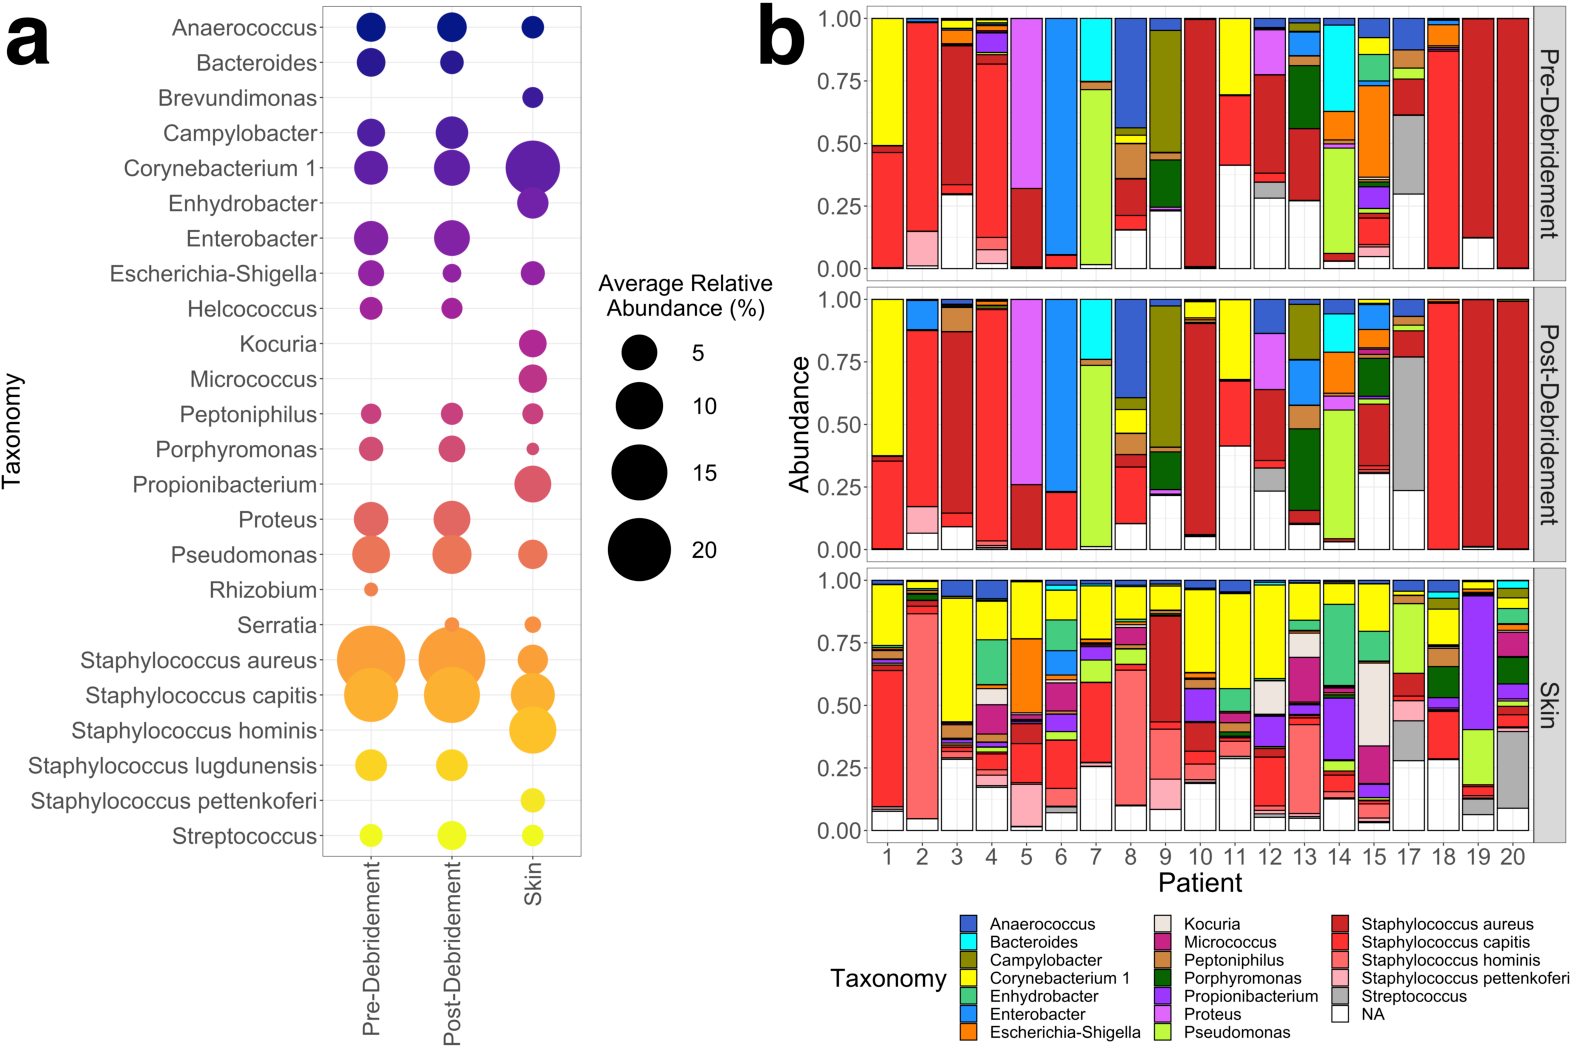
\includegraphics[width=\textwidth]{fig/C3fig1.pdf}}
\caption{Taxonomic composition of skin and wound samples. (a) Average relative abundance of genera within each sample type (only genera with average relative abundance $>1$\% are shown). \textit{Staphylococcus} taxa are labeled at the species level. (b) Relative abundance of genera in each sample (bar graph limited to the 20 most abundant taxa overall; ‘NA’ indicates OTUs without taxonomic classification; \textit{Staphylococcus} taxa are labeled at the species level).}
\label{fig:1AB}
\end{figure}
\end{subsection}
 
As expected based on previous studies \cite{RN6}, the microbiomes of wound samples were less diverse than those of skin samples (Figure \ref{fig:S3AB}). Average taxonomic richness of OTUs, as estimated by the Chao1 index, was significantly (approximately 10-fold) lower in wound samples than in skin samples). Visual inspection of the distribution of OTU abundances, as well as calculation of diversity by the Shannon index, which accounts for both OTU richness and abundance, indicated that wound samples tended to be dominated by a handful of constituents, while skin communities had a more even distribution of taxonomic abundance. 

% figure fka S3
\begin{figure}
\centering
\centerline{\includegraphics[width=\textwidth]{fig/C3figS3AB.pdf}}
\caption{Bacterial diversity of skin and chronic wound microbiomes. (a) Boxplots of richness (Chao1) and Shannon indices for each sample type indicate that while pre- and post-debridement wound samples have similar within-sample diversity, skin samples are significantly more diverse. Data points corresponding to a single patient are connected by grey lines. Averages were compared with paired, two-sided Wilcoxon signed-rank tests, resulting in the $p$-values shown. Error bars shown in the Chao1 plot are standard errors of the richness estimation. (b) Heatmap of relative abundance of the 300 most abundant OTUs.}
\label{fig:S3AB}
\end{figure}

A Bray-Curtis dissimilarity matrix was calculated from the OTU table of all samples and visualized by non-metric multidimensional scaling (NMDS). This non-phylogenetic ordination showed that skin samples form a distinct cluster that is separable from wound samples (Figure \ref{fig:S4AF}a). Indeed, pairwise Bray-Curtis dissimilarities between skin and wound samples were significantly different from zero (Figure \ref{fig:S4AF}b). Similarly, principal coordinates analysis (PCoA) using the unweighted UniFrac 36 distance matrix also results in clear partitioning of the skin samples from the wound samples, indicating that the skin samples share common community members across patients while the wound samples contain phylogenetically distinct taxa (Figure \ref{fig:S4AF}c). Averaged across patients, pre- and post-debridement wound samples had large unweighted UniFrac distances of $0.66 \pm 0.09$ ($\text{mean} \pm \text{standard deviation}$) and $0.67 \pm 0.08$ to the skin sample from the same patient, respectively (Figure \ref{fig:S4AF}d). However, when abundance is taken into account by PCoA ordination of the weighted UniFrac distance matrix (Figure \ref{fig:S4AF}e), skin and wound samples are less distinct from each other (average weighted UniFrac distances from pre- and post-debridement wound samples to the skin sample from the same patient were $0.33 \pm 0.12$ and $0.34 \pm 0.11$, respectively; Figure \ref{fig:S4AF}f), suggesting that high abundance taxa are shared between wound and skin while low abundance taxa distinguish skin from wound samples.

% figure fka S4 (only A-F)
\begin{figure}
\centering
\centerline{\includegraphics[width=\textwidth]{fig/C3figS4.pdf}}
\caption{Overall comparison of bacterial communities in skin vs. chronic wound microbiomes. Ordination based on the OTU table (normalized by relative abundance and filtered for OTUs with $>0.01$\% relative abundance in $>5$ samples) using Bray-Curtis dissimilarity (a), unweighted UniFrac (c), and weighted UniFrac (e) indicate that low abundance taxa distinguish skin (yellow cross) from wound samples (pre-debridement: red; post-debridement: aqua). Clinical wound type is indicated by marker shape, and each patient’s pre- and post-debridement samples are connected with black lines. Pairwise distances among sample types (pre-debridement, post-debridement, and skin) from the same patient, using Bray-Curtis (b), unweighted UniFrac (d) and weighted UniFrac (f) metrics. Averages were compared by Wilcoxon signed-rank tests ($p$-values shown) and data from each patient are connected by grey lines.}
\label{fig:S4AF}
\end{figure} 

To determine the extent to which low abundance taxa were unique to skin vs. wound samples, we counted the number of OTUs in each patient that were common or unique to skin or wound samples (pre- and post-debridement combined) from that patient. On average, wound samples contained $13.7 \pm 8.7$ wound-exclusive OTUs and shared $18.6 \pm 9.0$ OTUs with corresponding skin samples (Figure \ref{fig:S4GH}g). In contrast, skin samples contained $113 \pm 34$ skin-exclusive OTUs and shared $39.9 \pm 13.1$ OTUs with corresponding wound samples, indicating that most OTUs detected in a patient are exclusive to the skin while few OTUs are exclusive to the wound (Figure \ref{fig:S4GH}g). However, shared OTUs were disproportionately abundant in terms of community composition, accounting for an average of $98.2\pm5.3$\% of relative abundance in wound samples and $81.7 \pm 21.5$\% in skin samples, emphasizing that both skin and wound samples are largely composed of shared OTUs (Figure \ref{fig:S4GH}h). These results confirm earlier findings in chronic wound studies \cite{RN6, RN7, RN8, RN36}, verify the reliability of our samples, and exhibit reduced microbiome diversity similar to pathological states in other systems \cite{RN9, RN97, RN37}. 

% figure fka S4 (GH)
\begin{figure}
\centering
\centerline{\includegraphics[width=\textwidth]{fig/C3figS4GH.pdf}}
\caption{Overall comparison of bacterial communities in skin vs. chronic wound microbiomes. Number of OTUs (with average relative abundance $>0.1$\%) found exclusively on skin or wounds, or shared between both, per patient (a), and relative abundance of shared, skin- or wound-exclusive OTUs within each patient's samples (b).}
\label{fig:S4GH}
\end{figure} 

\begin{subsection}{Differences in abundance of individual bacterial taxa in skin vs. chronic wound microbiomes}
The individual taxa over-represented in skin or wounds are of interest for identifying potential keystone species or biomarkers of the healthy vs. diseased state. Several taxa appear to differ in abundance between skin and wounds (Figure \ref{fig:1AB}, Figure \ref{fig:S5}). Of taxa with average relative abundance $>1$\% across all patients, \textit{Proteus, Enterobacter, Campylobacter, Bacteroides,} and \textit{Helcococcus} were found almost exclusively in wounds. On the other hand, skin samples contained several major constituents not found in the wounds, including \textit{Propionibacterium, Enhydrobacter, Micrococcus, Kocuria,} and \textit{Brevundimonas}. Shared taxa also showed differences in abundance between skin and wounds. For example, \textit{Corynebacterium} was present in both skin and wounds, but its average relative abundance was greater on skin. Conversely, \textit{Staphylococcus, Porphyrmonas,} and \textit{Anaerococcus} were found on both skin and wounds, but their average relative abundances were much greater in wounds.

To determine the significance of such observations, we used DESeq2 and BGLMM to identify statistically significant associations of individual OTUs with wounds (pre-debridement) or skin. DESeq2 estimates the confidence interval of the log fold-change in abundance of each OTU between skin and wound samples, assuming count data follow a negative binomial distribution with dispersion estimated by combining data across OTUs \cite{RN32}. Analyzing a filtered OTU table (OTUs present in $>5$ samples with $>10$ counts; Figure \ref{fig:S1E}) using DESeq2, 97 out of 462 OTUs had significant differential abundance between skin and wounds (adjusted $p-\text{value } < 0.05$). Of these, 25 OTUs were enriched in wounds and 72 were enriched on skin. We focus on ‘abundant’ OTUs having average relative abundance $> 0.1$\% (11/25 of OTUs enriched in wounds and 32/72 of OTUs enriched in skin) (Figure \ref{fig:fig2}). To corroborate the DESeq2 analysis, we applied the Bayesian model BGLMM and used posterior credible intervals to identify significant associations. We validated BGLMM using simulations (Text S2). Applied to our data, BGLMM recapitulated the observed OTU counts reasonably well (Spearman’s correlation coefficient $> 0.75$; Figure \ref{fig:S6}). BGLMM found 54 OTUs with significant associations (i.e., 95\% credible intervals not including zero), with 50 being enriched in pre-debridement samples (22 being abundant) and only 4 being enriched in skin samples (3 being abundant) (Figure \ref{fig:fig2}). 

Despite some discrepancies between the two models, several abundant OTUs were identified by both analyses. For example, both models identified \textit{Staphylococcus aureus, Proteus, Enterobacter, Helcococcus} and \textit{Pseudomonas} genera as strongly enriched in wound (pre-debridement) samples, and \textit{Paracoccus, Micrococcus,} and \textit{Kocuria} as significantly enriched in skin samples. Compared to the qualitative description (Figure \ref{fig:1AB}), we validated that some OTUs from highly abundant genera ($> 1$\% relative abundance) that appeared to be exclusive to either wound or skin samples indeed were statistically significantly associated with either wound or skin. In particular, \textit{Proteus, Enterobacter,} and \textit{Helcococcus} were both exclusive to and significantly enriched in wound samples, while \textit{Kocuria} and \textit{Micrococcus} were both exclusive to and significantly enriched in skin samples. These associations and the variability among patients can be visually validated in the accompanying heat map (Figure \ref{fig:fig2}). In both models, significant OTUs comprise roughly half of the total abundance across the samples (Figure \ref{fig:S7}). 

% figure fka fig 2
\begin{figure}
\centerline{\includegraphics[width=0.9\textwidth]{fig/C3fig2.pdf}}
\caption{Association of abundant OTUs with pre-debridement wound samples or skin samples, inferred by DESeq2 or BGLMM. OTUs (with average relative abundance $>0.1$\%) found to be significant (criteria described in Methods) in at least one of the models with enrichment in wound samples (red) or enrichment in skin samples (blue). OTUs found to be not significantly enriched in that model are shown as gray. For DESeq2, the $log_{2}\text{fold-change}$ in variance-stabilized abundance is shown with estimated 95\% confidence interval ($1.96 \times \text{standard error}$). For BGLMM, the median of estimated $\beta_{j1}$ (pre-debridement effect for OTU $j$, see Methods for details) with 95\% credible interval are reported. The heatmap shows the $log_{10}(\text{relative abundance in wound minus relative abundance in skin})$ of each OTU of each patient for a visual comparison. OTUs are labeled by their genus name or lowest available taxonomy assignment if applicable; otherwise, the original OTU label from QIIME open OTU picking is used. Note that multiple OTUs may belong to the same genus.}
\label{fig:fig2}
\end{figure}

\end{subsection}

\begin{subsection}{Minimal changes to the chronic wound microbiome immediately after debridement}

The pre- and post-debridement wound microbiome samples were found to have similar diversity (Figure \ref{fig:S3AB}), and visual inspection of the community composition (Fig \ref{fig:1AB}b) suggests a high degree of similarity before and after debridement. However, the average unweighted UniFrac distance between pre- and post-debridement samples was substantial ($0.42\pm0.09$) (Figure \ref{fig:S4AF}d), although the average weighted UniFrac distance ($0.086\pm0.059$) was much smaller (Figure \ref{fig:S4AF}f). This pattern indicates that the major taxa are largely unchanged by debridement, but that there may be changes to the low-abundance taxa. This feature can be observed in the ordination analysis (Figure \ref{fig:S4AF}a,c,e), in which the pre- and post-debridement samples from each patient appear to cluster with each other in the weighted UniFrac and Bray-Curtis ordinations but not in the unweighted UniFrac ordination. 

To better understand the difference between pre- and post-debridement samples, we identified the OTUs in each patient that were unique to either the pre- or post-debridement communities vs. present in both. On average, a similar number of OTUs were found to be unique to pre-debridement samples ($13.8 \pm 11.4$) or unique to post-debridement samples ($12.0\pm5.3$), while $19.4\pm9.3$ OTUs were shared between the two (Figure \ref{fig:fig3ab}a). Consistent with the UniFrac metrics, OTUs unique to either pre- or post-debridement samples constituted a small proportion of overall composition ($2.04\pm5.52$\% and $1.17\pm3.66$\% on average, respectively) while shared OTUs accounted for the vast majority ($98.4\pm4.64$\%) of the sample composition on average (Figure \ref{fig:fig3ab}b). 

To determine whether individual OTUs were affected by debridement, regardless of uniqueness, we used DESeq2 and BGLMM to identify which OTUs were significantly associated with pre- or post-debridement samples (Figure \ref{fig:fig3cd}a). For OTUs with $> 0.1$\% relative abundance, \textit{Kocuria} (strict aerobes and facultative anaerobes) and \textit{Sphingopyxis} (strict aerobes) may be enriched in pre-debridement samples while the \textit{Comamonadaceae} family may be enriched in post-debridement samples. However, each association was detected by only one method, limiting overall confidence in these inferences.

% figure fka fig 3 ab
\begin{figure}
\centering
\centerline{\includegraphics[width=\textwidth]{fig/C3fig3AB}}
\caption{Comparison of pre- and post-debridement samples. Pre- and post-debridement samples have similar numbers of exclusive OTUs (a), and shared OTUs account for a large majority of microbiota (b).}
\label{fig:fig3ab}
\end{figure}


Since debridement was previously noted to affect anaerobes in particular after 2 weeks \cite{RN8}, we further characterized the oxygen requirements of the OTUs unique to pre- or post-debridement samples that also had an average relative abundance greater than 0.1\%. Note that post-debridement samples in this study were taken in the same clinic visit as pre-debridement samples, i.e., immediately after debridement. OTUs unique to pre-debridement samples included 10 aerobes (0.99\% average relative abundance), 6 anaerobes (0.44\% average relative abundance), and 5 facultative anaerobes (0.37\% average relative abundance). OTUs unique to post-debridement samples contained 7 aerobes (0.39\% average relative abundance), 2 anaerobes (0.28\% average relative abundance), and 2 facultative anaerobes (0.55\% average relative abundance). Although the number of taxa unique to pre- or post-debridement samples was small, the findings suggested a slight decrease of anaerobes post-debridement. To further probe whether anaerobes were immediately depleted by debridement, we grouped OTUs into the following four categories according to oxygen requirements: aerobes, anaerobes, facultative anaerobes, and taxa containing a mixture of these. None of these types showed a statistically significant difference between pre- and post-debridement samples using DESeq2 (Figure \ref{fig:fig3cd}b). Together these findings suggest that debridement by itself does not lead to an immediate alteration in the oxygen-requirement types comprising the wound microbiome, and changes, if any, to the taxonomic composition are likely to be small. 

% figure fka fig 3 cd
\begin{figure}
\centering
\centerline{\includegraphics[width=\textwidth]{fig/C3fig3CD}}
\caption{Taxonomic associations with pre- and post-debridement samples. (a) Analysis of statistically significant enrichment of individual taxa in pre- vs. post-debridement samples by DESeq2 and BGLMM; OTUs are sorted by descending average relative abundance. Note that \textit{Sphingopyxis} was only found to be abundant in patient 15. (b) Coarse-grained differential abundance analysis of aerobes, anaerobes, and facultative anaerobes using DESeq2 shows no significant difference immediately after debridement (error bars indicate 95\% confidence interval, or $1.96 \times \text{standard error}$). ‘Mixed’ indicates taxa that were not annotated due to: low relative abundance ($<0.1$\% on average), no taxonomic annotation, or ambiguous oxygen requirements.}
\label{fig:fig3cd}
\end{figure}
\end{subsection}

\begin{subsection}{Healing and non-healing wounds exhibit similar immediate response to debridement}
Chronic wounds were categorized into two groups based on whether the wounds had healed by 6 months after sampling (when medical record abstraction occurred for consented patients). Eight wounds fell in the ‘healed’ category and 12 in the ‘non-healing’ category. The age of the unhealed wounds was therefore known to be $>6$ months. Wound age was estimated using the time of first presentation as a proxy for the start of the wound. For healed wounds, wound age was known for 4 out of 8 patients; of those, two healed in $<12$ weeks of treatment and 2 healed after $6-9$ months. A previous study found that chronic wounds that healed within 12 weeks, but not wounds that did not heal within 12 weeks, showed a significant drop in Shannon diversity 2 weeks after debridement \cite{RN8}. In our samples, no significant change in bacterial diversity of the pre- and immediately post-debridement wound swabs was observed for either healing outcome (Figure \ref{fig:S8}a), suggesting that the previously observed drop in diversity reflects a gradual shift in the microbiome of healing wounds. Similarly, the microbiomes of healing and non-healing wounds did not differ in UniFrac distances to skin, indicating that the microbiomes of healing wounds did not exhibit a statistically significant overall similarity to the skin microbiome at this time point, compared to non-healing wounds (Figure \ref{fig:S8}b). 

The previous study \cite{RN8} also indicated that debridement appeared to decrease the abundance of anaerobes, as assessed 2 weeks post-debridement, in wounds that healed within 12 weeks, but not in wounds that did not heal in that time frame. It was therefore of interest to determine whether this differential response in anaerobes could be seen immediately after debridement. Following grouping into types of oxygen requirement (aerobes, anaerobes, facultative anaerobes), small but qualitatively similar trends were observed here. In wounds that healed, debridement caused a small decrease in the average relative abundance of anaerobes, from $16.1\pm24.1$\% pre-debridement to $13.6\pm18.8$\% immediately post-debridement (Figure \ref{fig:fig4AC}a), and a small increase in the average relative abundance of aerobes, from $61.5\pm25.9$\% pre-debridement to $66.6\pm21.4$\% immediately post-debridement (Figure \ref{fig:fig4AC}b). Unhealed wounds showed a slight increase in anaerobes and little change in aerobes from debridement (Figure \ref{fig:fig4AC}a,b). Debridement also caused little change in the relative abundance of facultative anaerobes (Figure \ref{fig:fig4AC}c). The small differences in response to debridement for the different oxygen-requirement types (anaerobes, aerobes, and facultative anaerobes) were not statistically significant for both healed and unhealed wounds (Figure \ref{fig:S9ABC}), supporting the idea that differences previously observed develop gradually over the days after debridement. 

% figure fka fig 4
\begin{figure}
\centering
%\hspace*{-1cm}
\includegraphics[width=\textwidth]{fig/C3fig4ACsq.pdf}
\caption{Comparison of healed and non-healing wounds. Average relative abundance of taxa classified by oxygen requirements (anaerobic (a), aerobic (b), and facultative anaerobes (c)) suggests facultative anaerobes may be predictive of healing outcome. Plots were filtered to show taxa with $> 0.5$\% average relative abundance within each sample type and outcome.}
\label{fig:fig4AC}
\end{figure}
\end{subsection}

\begin{subsection}{Differential abundance of facultative anaerobes in healed vs. unhealed wounds}
Although debridement did not appear to differentially affect the composition of oxygen-requirement types in healed vs. unhealed wounds among our samples, a large contrast was seen when comparing the relative abundance of facultative anaerobes in healed vs. unhealed wound samples (pre- or post-debridement). In unhealed wounds, the average relative abundance of facultative anaerobes was $20.8\pm29.7$\%, compared to $5.32\pm7.21$\% in healed wounds (Figure \ref{fig:fig4AC}c). This difference was not statistically significant using a two-sided Wilcoxon rank-sum test, indicating that there was no significant qualitative bias of facultative anaerobes in healed vs. unhealed samples. However, this non-parametric test is insensitive to the magnitude of the differences, i.e., heavy enrichment for facultative anaerobes may be associated with poor healing while mild enrichment has little effect. Examination of the data suggested a high variation in the abundance of facultative anaerobes among patients, especially those with unhealed wounds (Figure \ref{fig:fig4DEF}a). Indeed, the frequency distribution of facultative anaerobes was found to differ significantly between healed and unhealed wounds (Kolmogorov-Smirnov test: $p = 1.5 \times 10^{-4}$), and the variance in these distributions significantly differed from each other (Bartlett’s test: $p = 1.0 \times 10^{-6}$; Fligner-Killeen test: $p = 0.01$). We therefore analyzed the differential abundance of taxa having different oxygen requirements using DESeq2’s variance-stabilizing transformation, which can better account for heteroscedasticity of abundance across samples. Using DESeq2, we found that aerobes and especially facultative anaerobes are significantly more abundant in wounds that did not heal, while anaerobes are more abundant in wounds that did heal (Figure \ref{fig:fig4DEF}b).

To identify which specific OTUs were associated with healing outcomes, we applied DESeq2 and BGLMM method to compare the wound (pre- and post-debridement) samples of healed vs. unhealed wounds. Overall, most associations of individual OTUs with healing status were not consistently identified by both methods, likely due to the small sample size and diversity of wound colonization among patients. One result found by both methods is that \textit{Enterobacter}, a facultative anaerobe, is associated with non-healing (Figure \ref{fig:fig4DEF}c). We also applied DESeq2 to identify skin OTUs associated with healing outcomes. Only one OTU, \textit{Corynebacterium}, was significantly associated with healed wounds; none were associated with unhealed wounds (Figure \ref{fig:figS10}). 

% break this one up again - A and B together, make C separate and large
\begin{figure}
\centering
\centerline{\includegraphics[width=\textwidth]{fig/C3fig4DEF.pdf}}
\caption{Comparison of healed and non-healing wounds. Cumulative relative abundance of aerobes, anaerobes, facultative anaerobes, and unassigned taxa in wound samples that did or did not heal (a). Healed wounds are ordered by estimated wound age when known; unhealed wounds are ordered by treatment time up to the point of medical record data collection. Differential abundance analysis of healing outcomes for taxa with different oxygen requirements using DESeq2 indicated substantial enrichment of facultative anaerobes in non-healing wounds (b). Taxonomic associations (OTU with average relative abundance $> 0.1$\%) identified by BGLMM or DESeq2 with healed or unhealed wounds, comparing pre-debridement or post-debridement samples from each outcome, indicates significant enrichment of \textit{Enterobacter} in non-healing wounds (c).}
\label{fig:fig4DEF}
\end{figure}


\end{subsection}

\end{section}

%---  Discussion-------------------------
\begin{section}{Discussion}

We enrolled 20 patients with chronic wounds to characterize the microbial composition of the wound surface exposed by a single, sharp debridement event and assess whether microbial taxa could be predictive of clinical outcomes. While outcomes are certainly influenced by multiple host factors and other clinical factors, we focused on whether microbial taxa were associated with outcomes. Taxonomy summaries and diversity metrics of skin and wound microbiomes were consistent with previous reports \cite{RN6, RN7, RN8, RN36}. We applied a novel Bayesian generalized linear mixed model, in addition to DESeq2, to statistically assess associations of individual OTUs with specific sample types (see Text \ref{TextA1} for discussion of modeling methods).

BGLMM and DESeq2 agreed on the identification of several taxa that were strongly enriched in wound samples compared to skin. In line with prior assessments of skin and chronic wounds \cite{RN6, RN7, RN8, RN36}, the common skin commensals \textit{Micrococcus, Paracoccus,} and \textit{Kocuria} were significantly associated with skin using both methods, and DESeq2 further identified a number of \textit{Corynebacterium} and \textit{Staphylococcus} OTUs (\textit{S. hominis, S. haemolyticus, S. cohnii}) associated with skin. The known pathogens and wound colonizers \textit{Staphylococcus aureus, Staphylococcus capitis, Proteus, Enterobacter, Helcococcus} and \textit{Pseudomonas} were significantly associated with wounds by both methods. Notably, \textit{Staphylococcus} OTUs were associated with both skin and wounds, and species-level associations were only resolved after re-annotation of those OTUs using tools outside of the standard QIIME pipeline and SILVA128 database. This drawback highlights the utility of higher resolution 16S analysis methods and annotation, such as ‘amplicon sequence variant’ approaches \cite{RN97}, or shotgun metagenomics. This has been demonstrated in a recent study showing strain- and species-specific effects in the wound microbiome \cite{RN8}. Nonetheless, the agreement between DESeq2 and BGLMM on these results increases confidence in the associations identified here, and may prompt further testing of associations found by only one method. 

The practice of wound debridement is based on expected impacts on both host physiology and wound microbiota. We swabbed wound surfaces before and then immediately after a single, sharp debridement event in an outpatient clinic. No significant difference in the microbiome composition was detected, either in abundance of OTUs or in abundance of taxa grouped by oxygen requirement (aerobe, anaerobe, facultative anaerobe, and mixed/other/NA). Therefore, we infer that the prior finding of anaerobe depletion at 2 weeks post-debridement results from a gradual shift over days. It should be noted that the small size of this study limits its power to detect small community changes. In addition, Levine’s technique can sample exudate from deep tissue \cite{RN37}, so swabbing itself may disguise small differences in the wound before and after debridement. Nevertheless, the finding that the composition of the wound surface microbiome immediately exposed by sharp debridement is not significantly different from the pre-debridement wound suggests that the roles of host-associated factors, such as moderation of inflammation, as well as total microbial bioburden, warrant further study. Furthermore, these findings support the principle that debridement should be utilized frequently and aggressively to be most effective \cite{RN48}.

Wounds were followed up to $\sim 6$ months after sampling, enabling patients to be grouped by healing vs. non-healing outcome after 6 months. In this study, the outcome reflects time since sampling rather than true wound age. The ‘healed’ outcome therefore includes both wounds with age $\sim 6$ months as well as those with age $\sim 6$ months that originated before the time of sample collection and healed before patient data were collected. ‘Unhealed’ wounds all had age $\sim 6$ months. While 12 weeks after initial presentation has been used in other microbiome studies \cite{RN7, RN8} as the assessment time point to distinguish healed from unhealed wounds, 12 weeks was not a practical distinction in our study, in which few wounds healed within that time frame. 

When comparing the microbiomes (pre-debridement) of healed vs. unhealed wounds, a notable finding was the over-representation of facultative anaerobes as a group in the microbiome of non-healing wounds. In contrast, healed wounds appeared to be enriched for anaerobes. It is tempting to speculate that infections in which strict anaerobes play a key role are more easily cleared as the wound heals and the oxygen level increases in the tissue \cite{RN38}, disfavoring anaerobic organisms. On the other hand, infections in which facultative anaerobes play a key role, however, would be more tolerant to the changing conditions of a healing wound and may thus persist. This interpretation has implications for our understanding of treatments based on increasing the oxygen tension in the wound (e.g., hyperbaric oxygen \cite{RN39}), for which conflicting literature exists with regard to efficacy \cite{RN31}. In particular, the presence of pathogenic facultative anaerobes may render the wound refractory to oxygen therapies, suggesting that oxygen therapies should be targeted against wounds with low levels of facultative anaerobes. Another intriguing possibility is that facultative anaerobes may better tolerate the substantial oxygen gradients within the biofilm itself, causing persistence of the biofilm, as recent studies indicate that variable oxygen tension is a dominant stress in the high-density environment of the biofilm \cite{RN50, RN49}. In that case, the association of facultative anaerobes with non-healing would be a consequence of the selective environment within the biofilm. Alternatively, the association of facultative anaerobes with non-healing may reflect a correlation to a different feature that causes poor healing. For example, the facultative anaerobe metabolism may be an incidental trait in organisms that are particularly problematic in chronic wounds for other reasons. Aside from the mechanism, higher levels of facultative anaerobes may still be useful as prognostic markers of more resilient communities that inhibit healing. Further experimental studies would be needed to probe the influence of facultative anaerobes suggested here.

Taxonomic associations with wound healing are of special interest, as they may point toward species that, in combination with other host-related and clinical factors, promote or delay healing or which may act as biomarkers of healing status. The analyses of individual taxa by both DESeq2 and BGLMM revealed that the genus \textit{Enterobacter}, a facultative anaerobe, was associated with non-healing status. In addition, we did not observe \textit{Enterobacter} in normal skin from the patients in this study, i.e., \textit{Enterobacter} was exclusive to wounds. While \textit{Enterobacter} has been reported in chronic wounds \cite{RN10, RN13}, its potential role has been understudied relative to the more abundant \textit{Staphylococcus} and \textit{Pseudomonas} taxa. Interestingly, \textit{Enterobacter} species are a common causative organism of acute infections; in one study, Enterobacter was found to be a negative prognostic indicator for surgical site infections developed after neurosurgery \cite{RN40}. We suggest that further attention to the possible role of \textit{Enterobacter} in chronic wounds is warranted. 

Other taxonomic associations with healing outcomes were detected by only one method, likely due to the small sample size and natural heterogeneity of wounds among patients. BGLMM analysis indicated that healed wounds were positively associated with \textit{Brevundimonas}. DESeq2 appeared to be more sensitive to associations in general, with healed wounds positively associated with \textit{Anaerococcus, Peptoniphilus, Corynebacterium,} and \textit{Serratia}. DESeq2 also identified healing to be negatively associated with \textit{Enterococcus, Staphylococcus, Pseudomonas,} and \textit{Proteus}. The facultative anaerobe \textit{Proteus} is an intriguing candidate, because, like \textit{Enterobacter}, its overall abundance in non-healing wounds is relatively high (e.g., Figure \ref{fig:S9DE}). Additionally, a single \textit{Corynebacterium} OTU from skin samples was positively associated with healing. The less robust findings represent hypotheses that may be further tested in larger studies. The results also validate BGLMM as a novel statistical model complementary to DESeq2 for future association studies.

\begin{subsection}{Limitations}
The power of this study to identify correlations (or associations) was limited by its small cohort size (20 patients), such that only associations of relatively large effect would be detected. Larger cohorts will be important to test the findings, particularly correlations discovered by only one statistical method. Within patients, sampling was limited to one swab pre- and one swab post-debridement per wound, both due to the possibility of small wound sizes and concerns raised in discussion with the Institutional Review Board regarding repeated sampling. While limited sampling is a potential concern, the concordance between pre- and post-debridement samples found here suggests that swabbing itself is not a major source of variation. On the other hand, while all wounds underwent sharp debridement, the instrument used for debridement and degree of debridement were not controlled and may contribute to patient-to-patient variability in the results. 

Although we sequenced the V1-V3 loops of the 16S rRNA gene, taxonomic resolution was limited to the genus level for most OTUs. This is likely due to the OTU clustering threshold (97\% identity) and reference database (SILVA128). Additional analysis of OTUs of interest (\textit{Staphylococcus}) allowed tentative species-level annotation, although metagenomic sequencing would enable more confident assignments. 

Finally, the microbiome data collected here are compositional, i.e., absolute amounts of bacteria are unknown. While we know that negative control samples yielded undetectable amounts of DNA and nearly all skin and wound samples (59/60) yielded detectable amounts \cite{RN41}, quantitative information on bacterial loads would be useful for interpreting the detection of species (e.g., contamination from reagents) in the negative controls. In addition, bacterial load is likely to be affected by debridement, and correlation analysis might yield more physiologically relevant associations given absolute quantitative data. While swabbing may not be appropriate for absolute quantitation, microbiome sampling by other means (e.g., biopsy \cite{RN26}) might be more amenable. However, the relevance of quantitative microbiological data for clinical outcomes, and the techniques for collecting these data, are not yet clear \cite{RN24}. 
\end{subsection}
\end{section}

\begin{section}{Conclusion}
In summary, the results of this study show that sharp debridement does not have a large immediate impact on the composition of wound microbiota. In addition, the study identified the abundance of facultative anaerobes \textit{in toto} as a negative prognostic factor for healing in chronic wounds, and the facultative anaerobe \textit{Enterobacter} was specifically associated with non-healing vs. healing wounds. Understanding the mechanism of these associations will require causal inference (e.g., from time series data) and/or experimental models. Further work in these directions may be fruitful for understanding the contribution of the microbiome to wound healing as well as personalizing therapeutic recommendations based on wound-specific microbiomes.
\end{section}

%---  Methods-------------------------
\begin{section}{Methods}

\begin{subsection}{Ethics statement}
Clinical sample collection was performed at Ridley-Tree Center for Wound Management at Goleta Valley Cottage Hospital in accordance with protocols approved by the Cottage Health Institutional Review Board (Study Protocol 17-48u) and UCSB's Human Subjects Committee and Institutional Review Board (Study Protocol 4-18-0190). We recruited a cohort of 20 wound care patients over the course of a week and a half, and collected samples after obtaining informed, written consent from the patient.
\end{subsection}

\begin{subsection}{Collection of clinical samples}
Four clinically classified chronic wound types were sampled (diabetic ulcers, venous wounds, arterial wounds, and pressure ulcers), with five patients per wound type. Exclusion criteria were: patients under the age of 18, in the intensive care unit, or presenting with an unrelated non-wound infection. All patients underwent sharp debridement, but the extent and depth of debridement, as well as the type of instrument (curette, scalpel, scissors, or tissue nipper), was not standardized and was determined by the treating physician (Table \ref{Tab:woundsummary}). Debridement was not conservative and was undertaken until bleeding was observed. Sterile Copan FLOQSwabs 520C were pre-wetted with sterile PBS prior to all sample collections. During a single patient visit, wound swabs were collected pre-debridement and 1-2 minutes post-debridement, and a healthy skin swab was collected from the contralateral limb. Wound samples were collected from the area of debridement. All skin and wound samples were collected by employing Levine’s technique; gentle pressure was applied as the swab was wiped and rolled across a $\sim$ \SI{1}{\centi\meter\squared} area of healthy granulation tissue for approximately 30 seconds. Clinical swabs were placed back into the dry, sterile collection tube and stored at \SI{4}{\celsius} for no more than four hours before being processed. Negative control samples from the wound center were collected by exposing swabs to air in the collection room for the same duration as wound and skin swab collection. Processing control samples were obtained by exposing swabs to air and reagents in the processing lab analogously to clinical samples. A cell-based microbial mock community (Zymo) was included as a positive control.
\end{subsection}

\begin{subsection}{Sample processing \& DNA extraction}
Samples were transported to UCSB and processed following the protocol described in \cite{RN41}. Swabs tips were broken off into sterile \SI{1.5}{\milli\liter} microcentrifuge tubes, and samples were resuspended in \SI{500}{\micro\liter} sterile 1X TE by vortexing for 2 minutes at high speed on a multitube vortex adapter. Cells and cell debris were pelleted by centrifugation at $16,000 \times g$ for 2 minutes. \SI{250}{\micro\liter} of supernatant was transferred to a sterile microcentrifuge tube for virus-like particle enrichment and DNA extraction, while the remaining solution and swab tip were retained for whole microbiome DNA extraction. All subsequent purification and extraction steps were performed as described in \cite{RN41}. Briefly, bacterial DNA was extracted by high activity lysozyme treatment, proteinase K digestion, chemical lysis, bead beating, and final DNA purification with a PureLink Genomic Mini Kit, with all samples eluted into \SI{25}{\micro\liter} of 1x TE. Extracted DNA was quantified using a Qubit 3.0 instrument, dsDNA HS kit, and \SI{5}{\micro\liter} of sample. Of the 20 skin samples, only one sample was below the limit of detection (\SI{40}{\pico\gram}); the minimum total DNA detected was \SI{1}{\nano\gram}, maximum was \SI{17.3}{\nano\gram}, and average was \SI{3.0}{\nano\gram}. All wound samples produced sufficient DNA for Qubit quantification; the minimum total DNA detected was \SI{48.3}{\nano\gram}, maximum was \SI{11.5}{\micro\gram}, and average was \SI{2.92}{\micro\gram}. All negative controls were below the limit of detection, and positive controls yielded sufficient DNA for sequencing.
\end{subsection}

\begin{subsection}{Library preparation \& sequencing}
16S rRNA sequencing libraries were generated by two-step PCR for each sample. In the first step, V1-V3 loops were amplified using custom adapter primers composed of universal 16S primers ‘27F’ and ‘534R’ and Illumina Nextera indexing adapter sequences. Adapter PCR was done in \SI{25}{\micro\liter} reactions containing \SI{11.5}{\micro\liter} of template, \SI{0.5}{\micro\liter} of each primer at \SI{10}{\micro\molar}, and \SI{12.5}{\micro\liter} of KAPA HiFi HotStart ReadyMix. Adapter PCR was performed under the following conditions: denaturation/activation at \SI{95}{\celsius} for 3 minutes, followed by 25 cycles of denaturation at \SI{95}{\celsius} for 30 seconds, annealing at \SI{55}{\celsius} for 30 seconds, and extension at \SI{72}{\celsius} for 30 seconds. PCR products were purified with \SI{20}{\micro\liter} AMPureXP beads and eluted into \SI{50}{\micro\liter} of \SI{10}{\milli\molar} Tris pH 8.5. In the second step, Illumina Nextera XT indices were added by PCR in \SI{50}{\micro\liter} reactions containing \SI{5}{\micro\liter} of product from adapter PCR, \SI{5}{\micro\liter} of Index 1, \SI{5}{\micro\liter} of Index 2, \SI{25}{\micro\liter} of KAPA HiFi HotStart ReadyMix, and \SI{10}{\micro\liter} of water. 8 cycles of PCR were conducted under the same conditions as adapter PCR. Indexed samples were purified with \SI{56}{\micro\liter} of AMPureXP beads, eluted into \SI{25}{\micro\liter} of \SI{10}{\milli\molar} Tris pH 8.5, quantified with a Qubit dsDNA HS kit, normalized and pooled for multiplexing. All samples, including controls, were sufficiently amplified for sequencing. Final library QC was done using an Agilent TapeStation dsDNA 1000bp kit. The final libraries were sequenced in a single run on an Illumina MiSeq with PE300 V3 chemistry at UCSB’s Biological Nanostructures Laboratory (BNL) sequencing core.
\end{subsection}

\begin{subsection}{16S rRNA bioinformatic analyses}
Paired-end reads were uploaded to the QIIME AWS AMI (AMI ID: ami-1918ff72, “qiime-191”)\cite{RN81}. Initial quality analysis was performed with FastQC. Reads were quality controlled by trimming and quality filtering with trimmomatic using default settings \cite{RN82}. Read joining was performed with QIIME’s joining script (join\_paired\_ends.py), using the fastq-join algorithm with default settings. Joined reads were fed into the open OTU picking pipeline (pick\_open\_reference\_otus.py) using default settings. Taxonomy was assigned using the SILVA128 16S reference database clustered at the 97\% identity threshold \cite{RN35}. Representative sequences that could not be aligned using pyNAST were putative human contamination \cite{RN43} and excluded from the final BIOM table \cite{RN44}. The final BIOM table (without PyNAST alignment failures) contained 69 samples (60 experimental + 9 controls), with 22,753 OTUs representing 5,931,472 total counts (median = 65,588). For 608 OTUs annotated as \textit{Staphylococcus} at the genus level, species level annotations were generated using blastn \cite{RN51}. Representative sequences of each OTU were queried against the NCBI nr/nt nucleotide collection, subset to the \textit{Bacillus/Staphylococcus} group (taxid: 1385). For each OTU, blast results were parsed by sorting the hit table, in descending order, by bit-score, then e-value, and the highest hit for each OTU was retained. The Entrez Direct command line tool was used to obtain the taxonomy lineage corresponding to each accession number from the parsed hit table, and the species name was appended to the OTU table in R. 

For differential abundance analyses, the OTU table was filtered to keep only OTUs with least 10 reads in at least 5 samples (filtered table contained 462 OTUs). Three experimental samples contained less than 1000 counts; analyses with the samples excluded yielded similar results to analysis of the full data set, so they are included in the analyses described here. The skin sample from patient 16 contained an abnormally high number of OTUs, and its rarefaction curve did not saturate; this sample, and its associated wound samples, were removed from analysis (Figure \ref{fig:S1AD}). Results from DESeq2 and BGLMM were compared with and without patient 16 (Figure \ref{fig:figS11}) to confirm the robustness of taxonomic association analysis to the removal of patient 16 data. 
\end{subsection}

\begin{subsection}{Diversity and differential abundance analyses}

All diversity analyses were performed in RStudio. Briefly, the QIIME BIOM table, tree file, and mapping file were imported and converted to a Phyloseq object \cite{RN45}. Data was preprocessed to root the tree, reformat the taxonomy levels and strings, add species level annotations for \textit{Staphylococcus} OTUs, transform counts to relative abundance values, filter out controls and insufficiently sequenced samples, and pre-generate genus-agglomerated tables for downstream analyses. Taxonomic summaries (dotplots, barcharts, boxplots) were generated using the genus-agglomerated tables, with filters indicated in the figure captions. Alpha diversity plots were generated using raw, unfiltered, unrarefied tables. Beta diversity distances were calculated using a genus-agglomerated table with counts normalized by relative abundance, and filtered to retain OTUs with average relative abundance greater than 0.01\%. Differential abundance analyses were conducted using the DESeq2 package with the Wald test and parametric fitting \cite{RN32}. $log_{2}$(fold-change)s and adjusted $p$-values were extracted for each comparison using the contrast function. OTUs with adjusted $p$-values less than 0.05 were considered as significantly different in a differential comparison. 95\% confidence intervals (CI) were estimated by $1.96 \times \text{standard error (lfcSE)}$ reported by DESeq2 package. Note that OTUs whose 95\% CI does not include zero might not be significant by the standard of adjusted $p$-value, as $p$-values were further adjusted by the Benjamini-Hochberg correction for false discovery rate using DESeq2.

Additional packages utilized for analysis and figure generation in RStudio include: genefilter, ggplot2, ggpubr, reshape2, RColorBrewer, viridis, wesanderson, grid, gridExtra, plotly, scales, dplyr, magrittr, data.table, and ape. Additional packages in python include numpy, pandas, scipy, matplotlib, and biom-python.
\end{subsection}

\begin{subsection}{Bayesian generalized linear mixed model}
To further assess the association of OTU abundances with different sample types (pre-debridement, post-debridement, or skin) and outcomes (healed or unhealed), we modified the model in \cite{RN33} to analyze our data. Let $Y_{ikj}$ denote the detected count of OTU $j$ in sample $k$ from patient $i$ in the sequencing, $i = 1,\ldots,n$, $k = 1,\ldots,K$, and $j = 1,\ldots,j$. In our dataset, three samples were taken from each of the patients. We have n = 19 or 20, depending on inclusion or exclusion of patient 16, $K = 3$, and $J = 462$ (OTU table filtered for counts $> 10$ in $> 5$ samples). We assume a negative binomial distribution for $Y_{ikj}$, $Y_{ikj} \sim NB(\mu_{ijk},s_{j}$), where $\mu_{ijk}$ is the mean of $Y_{ikj}$ and $s_{j}$ is the overdispersion parameter. $s_{j}$ accounts for overdispersion of counts $Y_{ikj}$ and we have $Var[Y_{ikj}] = \mu_{ikj} + s_{j} \times {\mu_{ikj}}^{2}$. We use the normal skin sample as the reference group and consider a log linear model for $\mu_{ikj}$, $log(\mu_{ikj}) = r_{ik} + \alpha_{j} + u_{ij} + \beta_{j1}x_{ik1} + \beta_{j2}x_{ik2}$, where $x_{ik} = (x_{ik1}, x_{ik2})$ is a vector of covariates. In our study, we use two binary indicators to represent different sample types (i.e., $x_{ik} = (0, 0), (1, 0) \text{ and } (0, 1)$) mean the skin, pre-debridement, and post-debridement samples from patient $i$, respectively. Regression coefficients $\beta_{j1}$ and $\beta_{j2}$ are parameters that infer the effects of pre- and post-debridement states on the abundance of OTU $j$ relative to its abundance on normal skin, respectively. The difference in the coefficients $\beta_{j1} - \beta_{j2}$ can be used to infer the effect of debridement on OTU $j$. Here, $r_{ik}$ is the normalizing factor for sample $k$ of patient $i$. It accounts for different total counts in samples (e.g. sampling and sequencing depths); $\alpha_{j}$ is the baseline abundance of OTU $j$ that explains variability in the baseline OTU abundances; $u_{ij}$ is a random effect of OTU $j$ in patient $i$ that accommodates heterogeneity between patients. Since $u_{ij}$ is common for all samples taken from patient $i$, it also induces dependence between abundances of OTU $j$ in the samples of patient $i$. In Bayesian models, unknown parameters are random and specification of \textit{a priori} distributions for the random parameters (called prior distributions) is required. Bayesian models then update the distributions of the random parameters using observed data and yield a posteriori distributions (called posterior distributions). We assume prior distributions on our unknown parameters such as $r_{ik}, \alpha_{j} \text{ and } \beta_{jp}$, similar to those in \cite{RN33}. In particular, we assume independent Laplace distributions for $\beta_{jp} (p = 1, 2)$, resulting in Bayesian lasso. The Laplace prior is a sparse inducing prior that improves estimation of $\beta_{jp}$ and facilitates variable selection. We used 95\% posterior credible intervals of  $\beta_{jp}, p = 1, 2, \text{ and } \beta_{j1} - \beta_{j2}$ to identify significant associations for individual OTUs. We also assume Laplace distributions for $u_{ij}$. For details of the prior specification see \cite{RN33}.  Since the posterior distribution is not in a closed form, we used a Markov chain Monte Carlo method consisting of Gibbs and Metropolis steps to evaluate the posterior distribution. Median and 95\% credible intervals for all $\beta_{jp}$ were reported.  

We performed an additional analysis to assess the association of OTU abundances with different samples types in healed and unhealed wounds. We considered pre- and post-debridement samples only and used the BGLMM with two covariates, pre- and post-debridement, and healed and unhealed wounds. The covariates form four different groups: pre-debridement/unhealed, post-debridement/unhealed, pre-debridement/healed, and pre-debridement/unhealed groups. We used the pre-debridement/unhealed group as the baseline and then let $log(\mu_{ikj}) = r_{ik} + \alpha_{j} + u_{ij} + \beta_{j1}x_{ik1} + \beta{j2}x_{ik2} + \beta_{j3}x_{ik3}$ similar to the previous analysis. Here $\beta_{j1}$, $\beta_{j2}$, and $\beta_{j3}$ represent the effects of the remaining three groups on the abundance of OTU $j$ relative to that of the baseline group.  Difference between a pair of $\beta_{jp}$ ($p = 1,2,3$) can be used to infer difference of OTU abundances between groups.

For all inference using BGLMM, regression coefficients ($\beta_{jp}$) whose 95\% credible interval did not include zero were considered to have a statistically significant effect. We conducted inference on the filtered table (462 OTUs) with or without patient 16 for DESeq2 and BGLMM.
\end{subsection}

\end{section}


%=== Chapter 4  ============================================
\chapter{The Chronic Wound Virome and its Associations with Bacterial Communities and Healing Outcomes}\newpage
\label{Chapter 4}

%---  Abstract-------------------------
\begin{section}{Abstract}
Two leading impediments to chronic wound healing are polymicrobial infection and biofilm formation. Recent studies have characterized the bacterial fraction of these microbiomes, and have begun to elucidate compositional correlations to healing outcomes, yet the factors that drive compositional shifts are still being uncovered. The virome may play an important role in shaping bacterial community structure and function. Previous work on the skin virome determined that it was dominated by bacteriophages, viruses that infect bacteria. To characterize the virome, we enrolled 20 chronic wound patients presenting at an outpatient wound care clinic in a microbiome survey, collecting swab samples from healthy skin and chronic wounds before and after a single, sharp debridement procedure. We investigated the virome using a virus-like particle enrichment procedure, shotgun metagenomic sequencing, and a \textit{k}-mer-based, reference-dependent taxonomic classification method. Taxonomic composition, diversity, associations to covariates, and putative phage-host correlations are presented. We find that the wound virome is highly diverse, with many phages targeting known pathogens, and may influence bacterial community composition and functionality in ways that impact healing outcomes.
\end{section}

%---  Introduction-------------------------
\begin{section}{Introduction}
Chronic wounds (i.e., those that fail to exhibit reasonable healing progress within an expected time frame) are a growing source of morbidity and mortality worldwide \cite{RN2, RN3}. Although often overlooked as a comorbidity of a primary disease, such as venous insufficiency, peripheral artery disease, or diabetes, chronic wounds are pervasive and costly, affecting at least 6.5 million people and costing the healthcare system at least \$25 billion annually in the U.S. alone \cite{RN2, RN3, RN4}. Some of the leading impediments to healing of chronic wounds are infection, biofilm formation, and associated pathological inflammation \cite{RN5}. Chronic wounds, while not always infected, are frequently colonized by polymicrobial communities. Recently, many culture-independent studies have characterized the extended microbial diversity of skin and wounds \cite{RN6, RN7, RN8, RN9, RN10, RN11, RN12, RN13, RN14, RN15, RN16, RN17, RN18, RN19, RN20, RN21, RN22, RN23, RN24, RN25, RN26, RN27, RN28}. These studies have found that wound communities are primarily composed of \textit{Staphylococcus spp., Pseudomonas spp., Corynebacterium spp., Streptococcus spp., Anaerococcus spp.,} and \textit{Enterococcus spp.,} and numerous low-abundance taxa. However, significant inter-patient variability in the composition of the wound microbiome cannot be explained by covariates like age, race, sex, or wound etiology \cite{RN6, RN10}. Still, some studies have indicated that community composition may be associated with healing outcomes. Temporal instability and the transition between several distinct community structures was associated with positive healing outcomes \cite{RN7}, and communities with high proportions of aerobes and facultative anaerobes were associated with poor healing outcomes (Chapter \ref{Chapter 3}).

To better understand the correlations between community composition and healing outcomes, it will be important to identify and characterize the factors that influence community composition. The wound virome may play a key role in modulating microbial community dynamics, but it has not yet been characterized. Previous work on the human virome has determined that bacteriophages, viruses that infect bacteria, are dominant \cite{RN126, RN140}. This is notable, as the ability of bacteriophages to infect, kill, and modulate host function has been well described \cite{RN122, RN168, RN151} and may help explain inter-patient variability, associations to healing outcomes, community dynamics, and pathogenicity \cite{RN148, RN143, RN77, RN140}. To date, only one other study has investigated the healthy skin virome with virus-like particle (VLP) enrichment \cite{RN56}. Focusing on dsDNA viruses, they found that $91\%$ of putative viral contigs could not be taxonomically classified; among those that could be classified, most belonged to the order \textit{Caudovirales} and targeted \textit{Staphylococcus spp., Corynebacterium spp., Streptococcus spp., Propionibacterium spp.}, and \textit{Pseudomonas spp.}, and the most common virus infecting humans was papillomavirus. They also found that the virome composition and diversity was associated with the skin site (e.g., sebaceous or moist, occluded or exposed), and exhibited high intra-personal variance but less temporal variance at a given site. Other skin microbiome studies have validated these findings, although VLP-enrichment was not employed \cite{RN55, RN166}. Despite progress in describing the human virome in general \cite{RN126, RN142, RN140}, no studies have used VLP-enrichment methods and metagenomics to characterize the chronic wound virome.

Here, we investigate the viromes of 20 chronic wound patients presenting to an outpatient wound care clinic. Swabs were collected from chronic wounds before and after a single, sharp debridement event, along with a skin sample from the contralateral limb. For a detailed description of the cohort, see Table \ref{Tab:woundsummary}. Samples were fractionated to enrich for VLPs while retaining a separate bacterial fraction, as described in Chapter \ref{Chapter 2} \cite{RN41}. The VLP fraction was characterized by shotgun sequencing, with read classification and taxonomic abundance analysis performed with Kraken2 and Bracken, respectively, using a custom database containing the latest NCBI Viral RefSeq genomes and the Joint Genome Institute's IMG/VR viral metagenome database \cite{RN172, RN173, RN175, RN78}. The bacterial communities were characterized by Illumina sequencing of the V1-V3 loops of the 16S rRNA genes (detailed analysis of bacterial communities is reported in Chapter \ref{Chapter 3}). Viromes were analyzed using ecological diversity metrics and differential abundance analyses, and virus-host interactions were investigated with correlation analyses. We report the composition of dsDNA viromes in skin and wounds, and find that wounds harbor diverse viral communities, largely composed of bacteriophages. Additionally, we identify specific taxonomic and functional associations with healing outcomes, and describe bacteria-bacteriophage interactions within healed and unhealed wounds. The implications of these findings on our understanding of the pathophysiology of chronic wound microbiomes is discussed.
\end{section}

%---  Results-------------------------
\begin{section}{Results}
\begin{subsection}{Read processing and classification summary}
High-throughput sequencing of skin and wound samples, along with negative controls, resulted in $635,166,925$ total paired end reads ($9,623,741 \pm 5,091,161$ per sample, on average). Reads were quality and adapter trimmed, length filtered, and joined, resulting in $556,645,739$ pre-processed reads ($8,434,026 \pm 4,541,820$ per sample, on average), which equates to an overall read retention rate of $86.64\%$ ($87.49 \pm 9.92\%$ per sample, on average). To assess the overall taxonomic composition, reads were first classified against the full NCBI RefSeq database \cite{RN174}. Human and bacterial contamination was prominent ($6,794,663 \pm 2,588,627$ eukaryotic and $1,205,730 \pm 2,588,627$ bacterial reads, on average across all samples), but viral read abundances were still substantial, with $13,278 \pm 55,825$ reads classified as viral, on average (\ref{fig:figC4S1}). An additional $3,660 \pm 10,720$ reads remained unclassified, on average.

To better assess the viral content of the samples, reads were re-classified with Kraken2 against the NCBI Viral RefSeq database, followed by classification against JGI's IMG/VR database, a large, public viral metagenome repository \cite{RN175, RN78}. Taxon abundance estimates were again calculated with Bracken. Using this method, viral read classification was increased to $379,992 \pm 581,996$ viral reads per sample, on average. Two types of taxonomic classifications were assigned to each hit: a viral species designation as assigned by NCBI or IMG/VR, and a viral 'type' designation, which denotes host association for prokaryotic viruses and common viral family name for eukaryotic viruses. Additional information regarding the curation of taxonomic designations can be found in the methods.

Contamination by laboratory phages was expected, due to the low-biomass nature of these samples and the number of viral bioengineering experiments performed in spaces adjacent to the sample processing and library preparation bench. Indeed, negative controls were composed primarily of \textit{Escherichia} phage and unclassified viruses at the type level (Figure \ref{fig:C4F1}a, Figure \ref{fig:C4S2}a). At the species level, ambiguous \textit{Escherichia} phage and unclassified taxa were the most abundant, followed by known lab contaminants, such as \textit{Escherichia} viruses Lambda, DE3, T7, T4, and M13 (Figure \ref{fig:C4F1}b, Figure \ref{fig:C4S2}b). An initial decontamination procedure was implemented with the R package Decontam, which identifies taxa that are more prevalent in negative controls than true samples \cite{RN177}. Using the four sequenced negative control samples and a conservative decontamination threshold, Decontam identified 39 potential contaminants, but overlooked many of the lab contaminants, so these taxa were manually removed. Additional decontamination results can be found in the appendix (Figure \ref{fig:C4Sneglist}, Figure \ref{fig:C4S3}). Even after decontamination, many taxa had no known host association, accounting for $42.27 \pm 18.72\%$ average relative abundance (Figure \ref{fig:C4S4}). While the biological and clinical relevance of these taxa is certainly of interest, it is beyond the scope of this work to further characterize such viruses. Unless otherwise stated, the following results will focus on the 'defined' fraction of the virome, which has  species- or 'type'-level assignments.

% fig 1 (negative controls)
\begin{figure}[h]
\centering
\centerline{\includegraphics[width=\textwidth]{fig/C4fig1.pdf}}
\caption{Negative control composition boxplots. Relative abundance of each taxon in each of the four negative control samples, prior to decontamination; only taxa with $>0.1\%$ are shown at the type level (a) and $>0.5\%$ at the species level (b).}
\label{fig:C4F1}
\end{figure}
\end{subsection}

\begin{subsection}{Skin and wound viromes are dominated by bacteriophages targeting pathogens and commensals}
Averaging relative abundance across all skin and wounds, the most abundant viral 'types' were \textit{Proteus, Actinobaculum, Pseudomonas, Staphylococcus, Salmonella, Yersinia}, and \textit{Corynebacterium} phages (Figure \ref{fig:C4F2}a). Similarly, the most abundant species were \textit{Proteus} phage VB\_PmiS, unnamed \textit{Actinobaculum, Yersinia, Neisseria} and \textit{Staphylococcus haemolyticus} phages, as well as two \textit{Pseudomonas} phages (Figure \ref{fig:C4F2}b). Within the wound samples, the most prominent viral types were \textit{Proteus, Actinobaculum, Staphylococcus, Campylobacter, Yersinia, Pseudomonas} and \textit{Salmonella} viruses, while skin samples exhibited high relative abundance of \textit{Chryseobacterium, Neisseria, Staphylococcus, Yersinia, Bacillus, Pseudomonas, Salmonella, Corynebacterium}, and \textit{Streptococcus} viral types (Figure \ref{fig:C4F3}). The top viral types shared between skin and wounds were \textit{Staphylococcus, Yersinia, Pseudomonas} and \textit{Salmonella} phage. At the species level, wounds had greater abundances of \textit{Proteus} phage VB\_PmiS, an unnamed \textit{Actinobaculum} phage, \textit{Pseudomonas} virus phiCTX, and \textit{Staphylococcus} phages StauST398-5 and Sextaec. Conversely, the most abundant species on skin were unnamed \textit{Neisseria, Yersinia, Bacillus, Corynebacterium, Streptococcus} and \textit{Pseudomonas} phages (Figure \ref{fig:C4S5}). Among viruses that infect humans, papillomavirus was the most common.

% fig 2 (Overall taxonomy summary)
\begin{figure}[tp]
\centering
\centerline{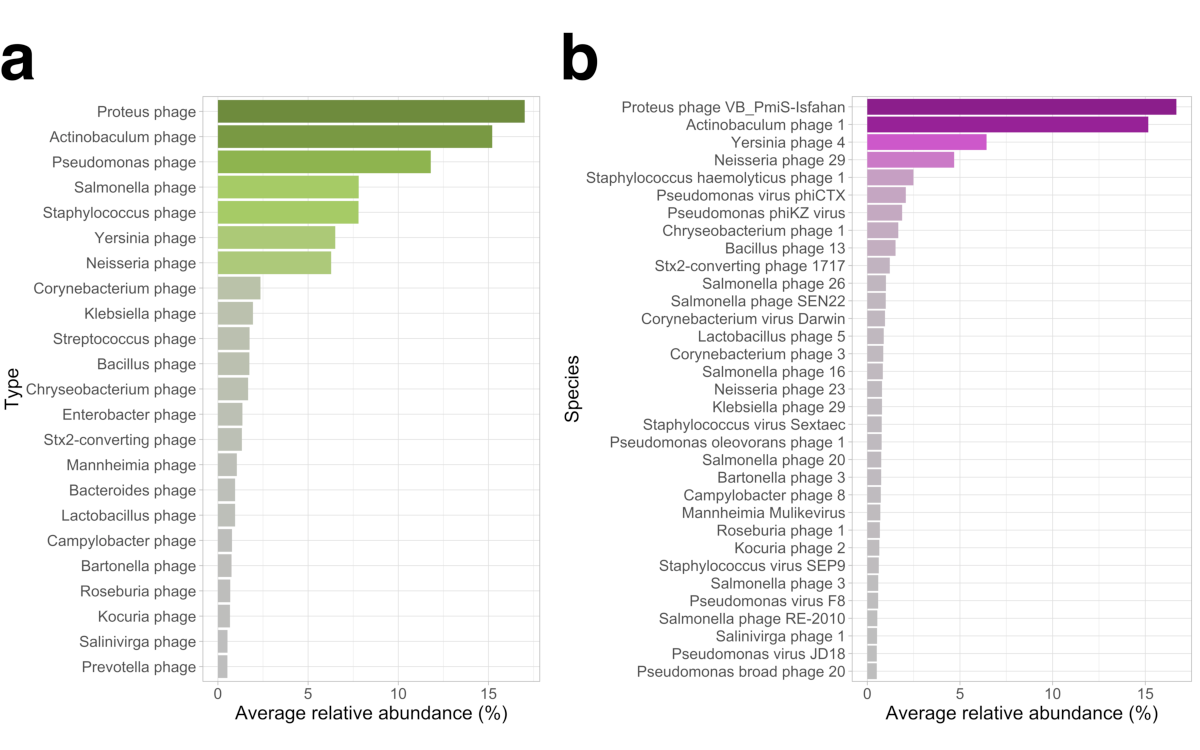
\includegraphics[width=\textwidth]{fig/C4fig2.pdf}}
\caption{Overall taxonomic composition of skin and wound viromes. Relative abundance of each taxon was averaged across all samples; those with $>0.5\%$ average relative abundance are shown here at the type level (a) and species level (b).}
\label{fig:C4F2}
\end{figure}


% fig 3 (Sample type taxonomy summary)
\begin{figure}[tp]
\centering
\centerline{\includegraphics[width=\textwidth]{fig/C4fig3.pdf}}
\caption{Taxonomic composition within sample types. Relative abundance of each taxon $>2\%$ at the 'type' level in pre-debridement, post-debridement, and skin samples.}
\label{fig:C4F3}
\end{figure}
 
\end{subsection}

\begin{subsection}{Wounds exhibit greater viral diversity than skin}
The virome exhibits significantly higher intra-sample taxonomic richness and evenness in wounds than skin, as measured by alpha diversity metrics with unclassified taxa included (Figure \ref{fig:C4F4}a). In terms of richness, wounds had an average Chao1 index of $996 \pm 426$ while skin had an average of $101 \pm 271$. Accounting for abundance and evenness, wounds had an average Shannon index of $4.70 \pm 0.72$ while skin had an average of $1.95 \pm 1.23$. The differences in richness and evenness can be qualitatively visualized as a relative abundance heatmap of the top 300 taxa (Figure \ref{fig:C4F4}b). The findings are in stark contrast to the bacterial fraction of skin and wound microbiomes, which exhibited an inverse relationship between alpha diversity of skin and wounds (Figure \ref{fig:C4F4}c). A correlation plot of bacterial and viral alpha diversity indicates that they are negatively correlated. It should be noted that, using the read based approach employed here, increased richness may be an artifact of homologous sequence alignments to unique but closely related taxa. Furthermore, decreased skin richness and evenness may be attributed to insufficient sampling due to the low-biomass nature of the environment.

% fig 4 (Alpha diversity)
\begin{figure}
\centering
\centerline{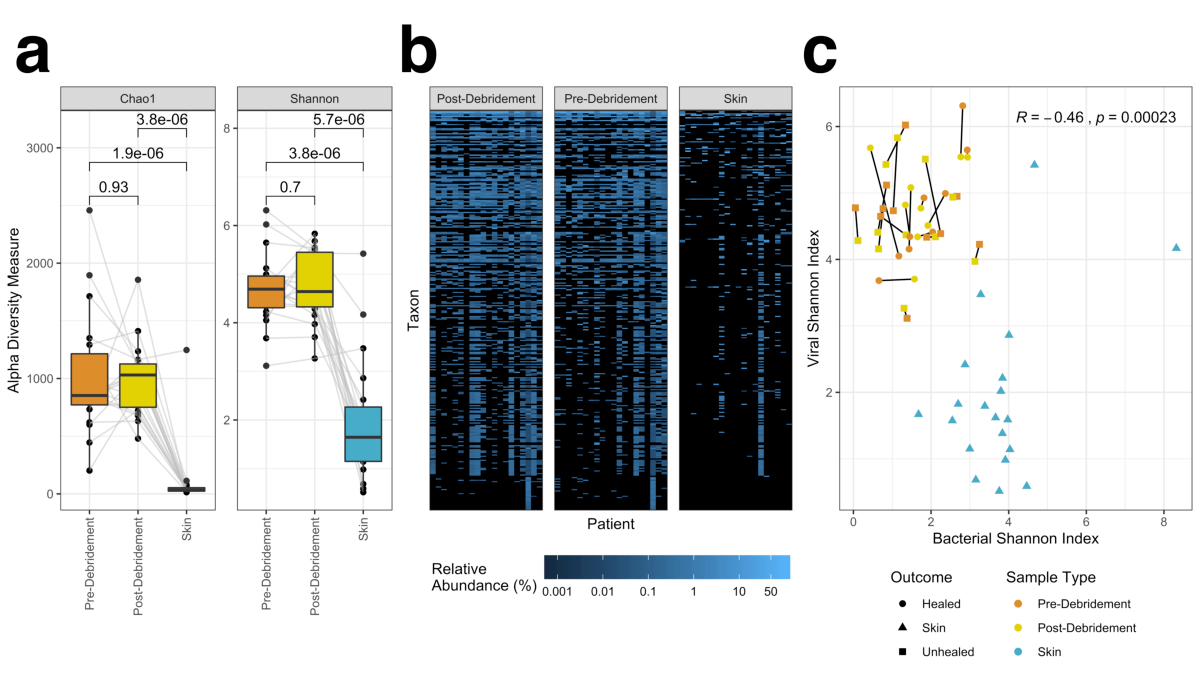
\includegraphics[width=\textwidth]{fig/C4fig4.pdf}}
\caption{Alpha diversity of skin and wound viromes. Boxplots of Chao1 and Shannon indices in wound samples (pre- and post-debridement) and skin samples with each patient's samples connected by grey lines, and averages compared with paired, two-sided Wilcoxon signed-rank tests, resulting in the \textit{p}-values shown (a). Heatmap of relative abundance of the top $300$ taxa in each patient's pre-/post-debridement and skin samples (b). Correlation between viral and bacterial Shannon indices with pre- and post-debridement samples from the same wound connected by a black line, sample type indicated by color, and outcome indicated by shape (c). Pearson's correlation coefficient \textit{R} and \textit{p}-value are shown, calculated using all samples.}
\label{fig:C4F4}
\end{figure}
\end{subsection}

\begin{subsection}{Skin and wound viromes are taxonomically distinct}
Diversity between samples can be measured using beta diversity indices, and visualized by ordination. Here, the Bray-Curtis distance is used with unclassified taxa included, and ordination is performed with principal coordinates analysis (Figure \ref{fig:C4F5}a). Examining the ordination, skin and wound samples are non-linearly partitioned, reinforcing the notion that they harbor distinct viromes, though there are some small overlaps indicating that some taxa are shared between sample types. Similar to the bacterial fraction, pre- and post-debridement samples are more closely related to each other than to their corresponding skin sample (Figure \ref{fig:C4F5}b). This finding also implies that, although the unclassified fraction of the virome has not been taxonomically described, it contributes to the diversity between skin and wound communities.

% fig 5 (Beta diversity)
\begin{figure}
\centering
\centerline{\includegraphics[width=\textwidth]{fig/C4fig5.pdf}}
\caption{Beta diversity as measured by Bray-Curtis dissimilarity. Taxa present in $>2$ samples with $>0.5\%$ relative abundance (including unclassified taxa) were retained for analysis. Ordination of the Bray-Curtis dissimilarity matrix using principal coordinates analysis (a). Within-patient dissimilarity between pre-debridement, post-debridement, and skin samples with averages were compared by Wilcoxon signed-rank tests (\textit{p}-values shown) and data from each patient are connected by grey lines (b).}
\label{fig:C4F5}
\end{figure}
\end{subsection}

\begin{subsection}{Viral species are associated with healing outcomes}
To identify specific taxonomic associations to covariates, differential abundance analysis was performed with DESeq2 (\ref{fig:C4F6}). Within wound samples, associations to healing outcomes are of primary interest. After filtering the results to retain associations with adjusted $p\text{-values}<0.01$, both healed and unhealed wounds were associated with specific \textit{Staphylococcus} phage. Healed wounds were also associated with many \textit{Pseudomonas, Campylobacter} and \textit{Bacteroides} phage, while unhealed wounds were associated with \textit{Enterococcus, Enterobacter, Veillonella} and \textit{Streptococcus} phage. Host association was known for these phages, but most did not have species designations approved by the International Committee on Taxonomy of Viruses (ICTV); instead, they had numeric species designations assigned by this study. 

For taxa with ICTV-approved species assignments, a literature review was conducted to infer their functional potential, revealing notable characteristics that may contribute to wound healing or pathogenesis (Table \ref{Tab:HUAssocTraits}). Both healed and unhealed wounds were largely associated with temperate phage in the family \textit{Siphoviridae}, including \textit{Staphylococcus} phages carrying Panton-Valentine leukocidin genes \cite{RN183, RN192}. Of the lytic phages, healed wounds were associated with two \textit{Staphylococcus} phage species and unhealed wounds were associated with \textit{Streptococcus} and putative \textit{Enterobacter} phage species. According to previous work, phage species associated with healed wounds may have profound impacts on host function, including reduction or inhibition of biofilm formation \cite{RN178, RN180}, motility inhibition equivalent to a pilus knockout \cite{RN178}, CRISPR resistance or inhibition \cite{RN179, RN180}, and anti-biofilm activity via capsid-displayed pectin lyase-like domains \cite{RN186}. 

% fig 6 (Outcome associations)
\begin{figure}
\centering
\centerline{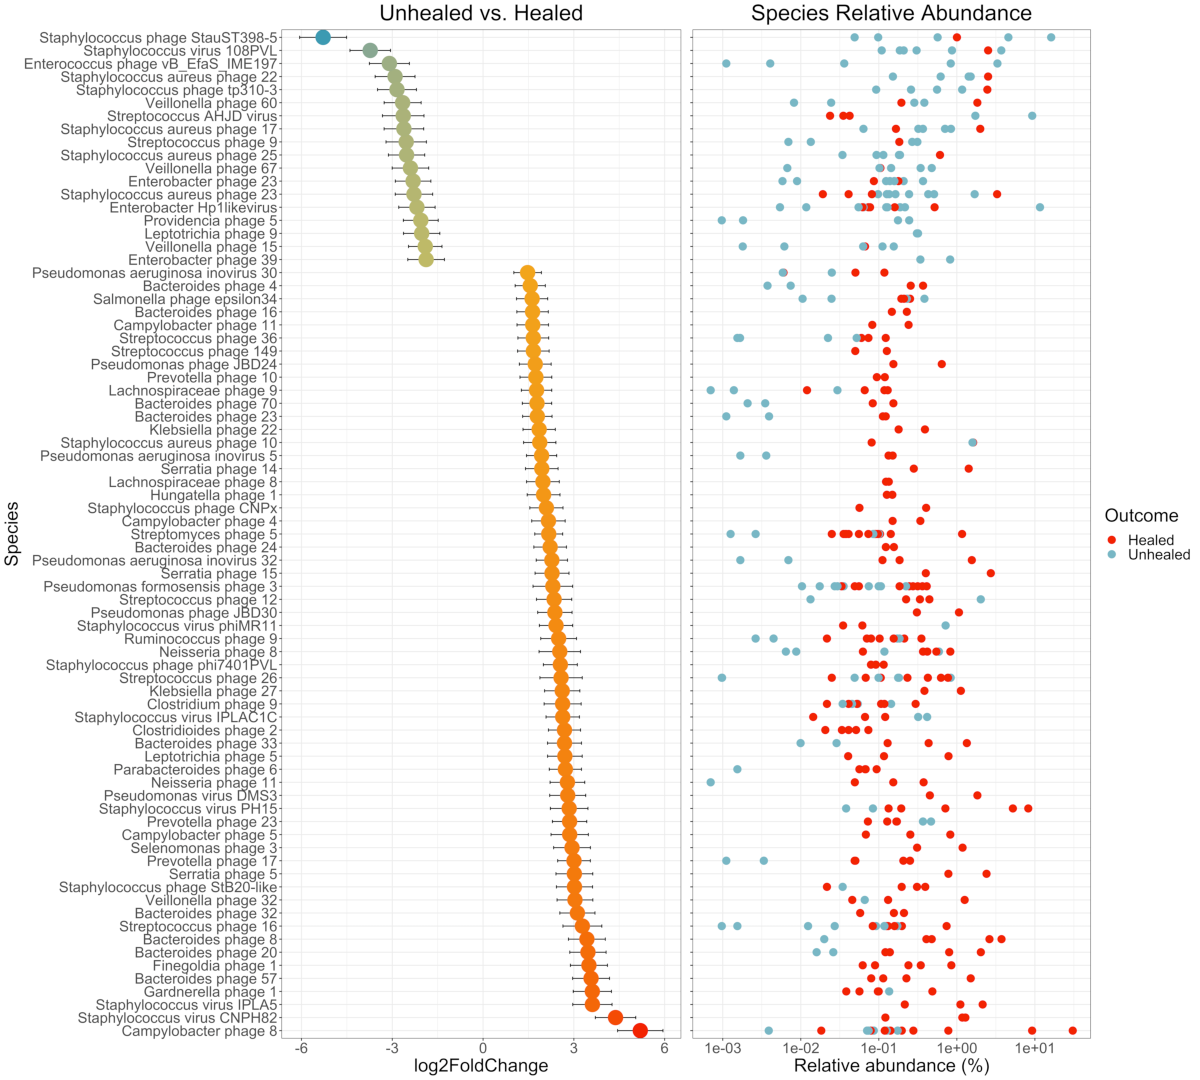
\includegraphics[width=\textwidth]{fig/C4fig6.pdf}}
\caption{Differential abundance analysis of healed and unhealed wounds with DESeq2. Associated species are represented by their log2FoldChange from the normalized, geometric mean calculated across all wound samples, contrasting unhealed (negative change) to healed wounds (positive change). Error bars represent the log-fold standard error. Only species with adjusted $p\text{-value}<0.01$ are shown. Relative abundance of each associated species, in each sample, are shown on the right; healed wound samples are red, unhealed wound samples are blue.}
\label{fig:C4F6}
\end{figure}

% table of healed/unhealed associated phage traits
\begin{table}[]
\caption{Traits of viruses associated to healed and unhealed wounds.}
\label{Tab:HUAssocTraits}
\footnotesize
\centering
\begin{tabular}{p{0.12\textwidth}p{0.18\textwidth}p{0.15\textwidth}p{0.1\textwidth}p{0.25\textwidth}p{0.04\textwidth}}
\hline
\textbf{Association} & \textbf{Species} & \textbf{Known hosts} & \textbf{Lifecycle} & \textbf{Notable traits} & \textbf{Ref.} \\
\hline
Healed & Pseudomonas phage JBD24 & \textit{Pseudomonas aeruginosa} & Temperate & inhibits motility (equivalent to pilus knockout); reduced biofilm formation & \cite{RN178} \\
Healed & Pseudomonas phage JBD30 & \textit{Pseudomonas aeruginosa} & Temperate & inhibits CRISPR systems & \cite{RN179} \\
Healed & Pseudomonas virus DMS3 & \textit{Pseudomonas aeruginosa} & Temperate & inhibits biofilm formation; exhibits CRISPR resistance & \cite{RN180} \\
Healed & Salmonella phage epsilon34 & \textit{Salmonella enterica subsp. enterica serovar} & Temperate & P22/Lambdoid phage (potential contaminant); alters \textit{Salmonella spp.} serotype & \cite{RN181} \\
Healed & Staphylococcus phage CNPx & \textit{Staphylococcus epidermidis} & Temperate & & \cite{RN182} \\
Healed & Staphylococcus phage phi7401PVL & \textit{Staphylococcus aureus} & Temperate & carries pore-forming toxin PVL & \cite{RN183} \\
Healed & Staphylococcus phage StB20-like & \textit{Staphylococcus epidermidis}; \textit{Staphylococcus hominis} & Temperate & & \cite{RN184} \\
Healed & Staphylococcus virus CNPH82 & \textit{Staphylococcus epidermidis} & Temperate & & \cite{RN185} \\
Healed & Staphylococcus virus IPLA5 & \textit{Staphylococcus epidermidis} & Lytic & pectin lyase-like domains; anti-biofilm activity & \cite{RN186} \\
Healed & Staphylococcus virus IPLAC1C & \textit{Staphylococcus ssp.} & Lytic & & \cite{RN187} \\
Healed & Staphylococcus virus PH15 & \textit{Staphylococcus epidermidis} & Temperate & & \cite{RN185} \\
Healed & Staphylococcus virus phiMR11 & \textit{Staphylococcus aureus} & Temperate & & \cite{RN188} \\
\hline
\hline
Unhealed & Enterobacter Hp1likevirus & \textit{Enterobacter} (putative) & Lytic & & \cite{RN189} \\
Unhealed & Enterococcus phage vB\_EfaS\_IME197 & \textit{Enterococcus faecalis} & Temperate & & \cite{RN190} \\
Unhealed & Staphylococcus phage tp310-3 & \textit{Staphylococcus aureus} & Temperate & & \cite{RN191} \\
Unhealed & Staphylococcus virus 108PVL & \textit{Staphylococcus aureus} & Temperate & carries pore-forming toxin PVL & \cite{RN192} \\
Unhealed & Staphylococcus virus StauST398-5 & \textit{Staphylococcus aureus} & Temperate & & \cite{RN193} \\
Unhealed & Streptococcus AHJD virus & Group C \textit{Streptococci} & Lytic & & \cite{RN194} \\
\hline
\end{tabular}
\end{table}
\end{subsection}

\begin{subsection}{Specific viral species are associated with skin and wound samples}
Species associations to skin and wound sample types were also explored. Although unique species were associated with each sample type, the hosts they targeted were largely shared, including \textit{Yersinia spp., Neisseria spp., Pseudomonas spp., Streptococcus spp., Salmonella spp.}, and \textit{Staphylococcus spp.} (Figure \ref{fig:C4S6}). Nevertheless, skin and wounds differed in some of the host species targeted. Skin was associated with one \textit{Staphylococcus haemolyticus} phage, one \textit{Staphylococcus aureus} phage, and two general \textit{Pseudomonas} phages, while wounds had many associations to \textit{Staphylococcus aureus} and \textit{Pseudomonas formosensis} phage species.
\end{subsection}

\begin{subsection}{Phage abundances are both positively and negatively correlated to host abundances}

To elucidate bacteria-bacteriophage interactions, correlation analyses can be performed. Comparing bacteriophage relative abundance to their host relative abundance hints at many types of interactions, with several overall correlations (i.e., across skin and wounds combined) found to be significant with Spearman's correlation coefficient. \textit{Bacteroides, Campylobacter,  Corynebacterium, Enterobacteria, Neisseria} and \textit{Pseudomonas} bacteria-bacteriophage pairs all had significant positive correlations. Among bacteria-bacteriophage pairs displaying negative correlations, the only one was significant (\textit{Actinobacteria}), though \textit{Propionibacterium} and \textit{Staphylococcus} pairs also displayed slight negative correlations.

Overall correlations are useful for identifying general trends, but they cannot discern special cases that hint at potential bacteria-bacteriophage interactions associated with covariates, or unique cases in individual patients. For example, some co-occurrence or exclusion relationships were related to sample type. For instance, skin samples had high \textit{Actinobacteria} relative abundance but almost no corresponding bacteriophage, while the inverse was true for the wound samples. Several healed wounds exhibited relatively high abundance of phage targeting abundant pathogens compared to other samples, including \textit{Campylobacter, Staphylococcus, Corynebacterium}, and \textit{Bacteroides}. Two patients had comparably high \textit{Pseudomonas} abundance, yet the patient with less phage abundance healed. The opposite was true for \textit{Bacteroides}, where two patients had comparable bacterial abundances, but the patient with higher phage abundance healed. For \textit{Proteus}, two patients with high bacterial abundance and phage did not heal, yet \textit{Proteus} phage was abundant in many healed samples that had negligible bacterial abundance.



% fig 6 (RA correlations b/w phage and host)
\begin{figure}
\centering
\centerline{\includegraphics[width=\textwidth]{fig/C4fig7.pdf}}
\caption{Relative abundance correlations between bacteriophage and their hosts. Viral relative abundance was agglomerated at the 'type' level for all phage targeting the same host, and bacterial relative abundance was agglomerated at the taxonomy level corresponding to the name of the plot. Relative abundances for corresponding phage/host pairs were plotted for each sample, with color representing sample type, shape representing healing outcome, and wound samples from the same patient connected by black lines. Spearman correlation coefficients were calculated for all samples combined, resulting in the \textit{R} and \textit{p}-values shown.}
\label{fig:C4F7}
\end{figure}

\end{subsection}

\end{section}

%---  Discussion-------------------------
\begin{section}{Discussion}
Using high throughput deep sequencing, we investigated the skin and chronic wound viromes of $20$ patients presenting at a wound care clinic. Samples were processed using a virus-like particle enrichment protocol in attempt to reduce host contamination and increase viral sequencing depth. We report the taxonomic composition of the viromes, associated ecological diversity measures, specific taxa associated with healing outcomes and sample types, and virus-host correlations. The present work is the first to investigate chronic wound viromes, and accordingly, the preliminary findings raise more questions than they answered, while also identifying many potential pitfalls.

Host contamination was estimated by classifying reads against the full NCBI RefSeq database, ultimately indicating a very high degree of human and bacterial contamination. While this method is suitable for estimating host contamination, true viral read abundances may have been obscured by alignment to CRISPR spacers and prophages in bacterial reference genomes, which are pervasive and have been well-documented \cite{RN80, RN133}. Additionally, NCBI's viral reference database is limited, and the remaining unclassified reads may have had viral origin. Despite implementation of VLP-enrichment procedures and the opportunities for viral read depletion, host contamination was notably prevalent, underscoring the importance of thorough host DNA degradation during sample processing.   

Viral detection and classification was performed with unassembled reads in a \textit{k}-mer-based, reference-dependent manner, though a viral metagenome database was utilized in an effort to capture relatively new or poorly annotated viruses. Indeed, approximately half of viral taxa detected had no known host or species annotation, in agreement with previous work in the field \cite{RN56, RN79}. This finding underscores one of the main drawbacks of this detection and classification method; it hints at the presence of a large, unclassified fraction of viral material, yet reads alone cannot be used to identify and annotate putative novel viruses. Future work should endeavor to better identify and classify putative viruses with read assembly, protein homology searches, and other methods described elsewhere \cite{RN132, RN133, RN134, RN135, RN136, RN154}. Of the viral taxa that were annotated, most targeted abundant skin and wound bacteria such as \textit{Proteus spp., Actinobacteria., Pseudomonas spp., Staphylococcus spp., Corynebacterium spp., Streptococcus spp.} and mixed Proteobacteria. This is a somewhat expected result, as the methodology applied here aimed to capture free viruses, which would have to be actively propagating by lysis of their host. Therefore, it also follows that wounds had more pathogen-targeting phages, while skin was associated with phages targeting commensals and putative contaminants, as those were the prominent bacterial taxa detected in the respective sample types using 16S rRNA sequencing.

With the unannotated viral taxa included in the dataset, wound viromes were significantly more diverse than skin in both taxonomic richness and evenness. Overall, viral diversity was negatively correlated with bacterial diversity. Taken at face value, this finding implies that high phage diversity may reduce bacterial diversity, or high bacterial diversity suppresses phage diversity. However, this correlation could be an artifact of insufficient viral sampling depth of skin. Even if the low viral alpha diversity of skin is an artifact, it suggests that the wound environment is hospitable to phage proliferation and may carry a higher viral burden than skin. Wound treatment may encourage further phage proliferation, as previous work has established that lysogenic phage may switch to the lytic lifecycle in response to antibiotics \cite{RN159}, reactive oxygen species \cite{RN158}, DNA damage signaled by SOS responses \cite{RN157}, and various stress responses to changes in the environment, like pH \cite{RN160, RN161}. Skin and wound viromes were also non-linearly partitioned by beta diversity ordination, suggesting they did not share major taxa, but there was a small overlap. These findings indicate that the skin and wound viromes are largely divergent, though dormant or ultra low-abundance taxa from skin may have increased abundance in wounds. 

Taxonomic associations were further characterized by differential abundance analysis. Associations to healing outcomes were particularly of interest, and several notable taxa displayed unique functional properties that could influence healing outcomes. Both healed and unhealed wounds were mostly associated with phages in the \textit{Siphoviridae} family, which are largely temperate, suggesting that there may be a shift in lifecycle in the wound environment. Furthermore, as temperate phages, \textit{Siphoviridae} may exert influence over their hosts' function through prophage integration and lysogenic conversion \cite{RN151, RN156}. In healed wounds, notable features included inhibition of biofilm formation and cell motility \cite{RN178, RN180}, proteolytic activity against extracellular matrix proteins \cite{RN186}, and suppression or inhibition of CRISPR systems \cite{RN179, RN180}. Biofilms are a leading impediment to wound healing, and exploitation of phage or their proteins as anti-biofilm agents is a very active area of research \cite{RN146, RN147, RN148, RN149}. Suppression of the CRIPSR system confers a great advantage to the bacteriophage by evading degradation by the host. Recent work suggests that anti-CRISPR systems are dependent on multiplicity of infection, requiring several phage to be expressing the gene simultaneously in a rare case of inter-phage cooperation and altruism \cite{RN150}. 

Both healed and unhealed wounds were associated with phage known to transduce the pore-forming toxin Panton-Valentine leukocidin, which may increase pathogenicity of their hosts by evading immune response and lysing leukocytes, though the specific role of leukocidins in wound pathogenesis is still unclear \cite{RN152}. Although not identified as associated to any particular group, \textit{Proteus} phage Phage vB\_PmiS-TH was prominent among wound samples. This \textit{Siphoviridae} phage has been found to be lytic against \textit{P. mirabilis}, a known wound pathogen, and may be a common wound commensal phage \cite{RN196}. It should be noted that these functional associations were not directly detected from the sequencing data, but rather inferred from the literature given the species designation of the viral hit. Future studies will benefit by identifying the specific functions of the virome through gene annotation of assembled reads. Still, these findings may guide future work as to which functional pathways and genes to investigate further. 
 
Phage-host correlations hinted at a variety of dynamics in both skin and wounds. Most overall correlations were indicative of co-occurrence relationships, similar to those described by the 'Kill-the-Winner' (KtW) model, which postulates that lytic phage abundance increases with host abundance and any apparent growth is offset by predation \cite{RN162}. Yet many phage species identified in the association analysis were temperate, and may adhere to the 'Piggyback-the-Winner' (PtW) model of phage growth \cite{RN155}. In this paradigm, temperate phage preferentially adopt the lysogenic lifecycle when bacterial growth rates are high, exploiting bacterial replication to proliferate as a prophage. Married with the 'bacteriophage adhesion to mucus' (BAM) model of immunity, PtW argues that low-abundance pathogens are quickly lysed while high-growth commensals retain their immunity \cite{RN155}. The BAM model also postulates that commensals use spontaneous induction to maintain a reservoir of lysogenic phage to attack invading pathogens, as a form of innate immunity for human hosts \cite{RN144}. This may begin to explain the large difference in skin and wound viromes; perhaps the ultra-low abundance lysogens from skin commensals are predating on wound pathogens. While it is tempting to speculate about potential evidence of KtW and PtW in these correlations, proper statistical inferences are hindered by the small-cohort, single-timepoint study design and low taxonomic resolution of both bacteria and phage. In reality, a messy combination of these models is likely at play, with high inter-personal and temporal variance.

\begin{subsection}{Limitations}

As with the investigation of the bacterial fraction, the statistical power of the viral investigation was limited by the small cohort size, and only associations of relatively large effect could be detected. The findings of this study should be validated with larger cohorts, using multiple statistical methods for association and correlation inferences. Viruses utilize a variety of genome morphologies, but this study focused exclusively on free, non-enveloped dsDNA viruses, with potential to capture replicative intermediates of ssDNA virues; enveloped viruses, prophages, and RNA and ssDNA viruses merit further investigation. Here, we determined viral abundance and taxonomy using a \textit{k}-mer-based approach at nucleotide sequence level with unassembled reads, which likely reduced the accuracy of both metrics due to the modular nature of viral genomes. This method is facile, but has potential for false-positive viral detection. Furthermore, viral detection, taxonomic classification, and host associations were limited by reference database dependence. The NCBI Viral RefSeq database is small, but curated and well-annotated, while IMG/VR is large but poorly annotated, and the degree of curation is unknown. It is well-known that temperate bacteriophage may excise portions of the host genome when entering the lytic lifecycle \cite{RN151, RN161}; if these bacterial sequences were present in the IMG/VR database, bacterial contaminants in the sample data may have appeared as false-positive viral hits. 

This work was also limited by significant host and environmental contamination, despite the use of viral enrichment protocols, extensive preventative measures, and exhaustive \textit{in silico} decontamination. Contamination is a common issue, especially when working with low-biomass clinical metagenomic samples, but nonetheless, it may have confounded some inferences made here \cite{RN71, RN70}. Contamination abundance was negatively correlated to extracted DNA mass, which is especially problematic for skin samples, which had the lowest DNA yields. Further complicating contamination issues, many putative contaminants reported in the literature are common skin microbiota, in the same genus as relevant clinical pathogens, or environmental microbiota that may truly be found on exposed skin or wounds. Additional measures, such as more robust extra-viral nuclease treatment and novel statistics-based \textit{in silico} decontamination methods, will improve the signal-to-noise ratio in future work.

\end{subsection}
\end{section}

%---  Conclusion-------------------------
\begin{section}{Conclusion}
Chronic wounds are frequently colonized and infected by polymicrobial communities, impeding wound healing. Previous work has established that the bacterial fraction of these communities exhibits high interpersonal variance, and community structure and function may be associated with healing outcomes. Yet the forces that drive compositional and functional dynamics of wound microbiomes have yet to be elucidated. We sought to better understand the role of a potentially important contributing factor, the virome. This study presents the first characterization of the chronic wound virome, utilizing a virus-like particle enrichment protocol and shotgun metagenomics to survey the wounds of 20 patients presenting at an outpatient wound care clinic. Despite heavy host contamination, we describe viral taxonomic composition, diversity, associations to covariates, and virus-host correlations. 

While no causative or conclusive claims can be made regarding the virome's role in wound pathology, the rich inter- and intra-personal taxonomic diversity and associations to covariates suggest that the virome is a prominent component of the greater microbiome and merits thorough investigation in the future. To achieve more sensitive viral detection and accurate taxonomic classification, future studies would benefit from shotgun sequencing both the bacterial and viral fractions of the microbiome, and assembling the resulting reads into contiguous sequences, which will facilitate protein homology searches and within-sample CRISPR spacer and prophage alignments. Furthermore, time series data will be imperative for elucidating the multitude of complex, dynamic bacteria-bacteriophage interactions. Such work will contribute to the greater understanding of how the wound microbiome as a whole is related to wound pathology, and ultimately, how it may be leveraged to achieve more positive healing outcomes.

\end{section}

%---  Methods-------------------------
\begin{section}{Methods}

\begin{subsection}{Ethics Statement}
Clinical sample collection was performed at Ridley-Tree Center for Wound Management at Goleta Valley Cottage Hospital in accordance with protocols approved by the Cottage Health Institutional Review Board (Study Protocol 17-48u) and UCSB's Human Subjects Committee and Institutional Review Board (Study Protocol 4-18-0190). A cohort of 20 wound care patients were recruited over the course of a week and a half, and samples were collected after obtaining informed, written consent from the patient.
\end{subsection}

\begin{subsection}{Clinical sample collection}
Four clinically classified chronic wound types were sampled (diabetic ulcers, venous wounds, arterial wounds, and pressure ulcers), with five patients per wound type. Exclusion criteria were: patients under the age of 18, in the intensive care unit, or presenting with an unrelated non-wound infection. All patients underwent non-conservative sharp debridement until bleeding was observed. However, the extent and depth of debridement, as well as the type of instrument (curette, scalpel, scissors, or tissue nipper), was not standardized and was determined by the treating physician (Table \ref{Tab:woundsummary}). Sterile Copan FLOQSwabs 520C were pre-wetted with sterile PBS prior to all sample collections. During a single patient visit, wound swabs were collected pre-debridement and 1-2 minutes post-debridement, and a healthy skin swab was collected from the contralateral limb. Wound samples were collected from the area of debridement. All skin and wound samples were collected by employing Levine’s technique; gentle pressure was applied as the swab was wiped and rolled across a $\sim$ \SI{1}{\centi\meter\squared} area of healthy granulation tissue for approximately 30 seconds. Clinical swabs were placed back into the dry, sterile collection tube and stored at \SI{4}{\celsius} for no more than four hours before being processed. Negative control samples from the wound center were collected by exposing swabs to air in the collection room for the same duration as wound and skin swab collection. Processing control samples were obtained by exposing swabs to air and reagents in the processing lab analogously to clinical samples.
\end{subsection}

\begin{subsection}{Sample processing and DNA extraction}
Samples were processed as described in Chapter \ref{Chapter 2} \cite{RN41}. Briefly, swab tips were inserted into \SI{1.5}{\milli\liter} microcentrifuge tubes and snapped at the \SI{30}{\milli\meter} break-point. \SI{500}{\micro\liter} of sterile 1X TE was added to the tube, and the tube was vortexed for 2 minutes at maximum speed on a multitube vortex adapter to resuspend the sample. Samples were then centrifuged at $16,000 \times g$ for 2 minutes to pellet cells. \SI{250}{\micro\liter} of supernatant was transferred to a \SI{2}{\mL} microcentrifuge tube for immediate VLP precipitation. The remaining \SI{250}{\micro\liter} of supernatant, pelleted cells, and swab tip were kept in the original tube and stored at \SI{-20}{\celsius} before proceeding to whole-microbiome DNA extraction.
\end{subsection}

\begin{subsection}{Isolation of DNA from virus-like particles}
VLP purification and DNA extraction was conducted as described in Chapter \ref{Chapter 2} \cite{RN41}. Briefly, free DNA in the VLP fraction was digested with DNase I (5 units, NEB) at \SI{37}{\celsius} for 30 minutes; DNase I was inactivated by incubation at \SI{75}{\celsius} for 10 minutes. VLPs were precipitated, pelleted, washed with ice cold 70\% ethanol, and re-pelleted. Pellets were dried for 1 hour at room temperature in a vacufuge before being resuspended in sterile 1X TE (pH 8.0). Viral capsids were disrupted and digested with 10\% SDS and proteinase K, incubated at \SI{55}{\celsius} for 1 hour. VLPs were further disrupted with \SI{5}{\molar} NaCl and CTAB-NaCl, followed by incubation at \SI{65}{\celsius} for 10 minutes. The sample was then transferred to a phase lock gel tube (5PRIME PLG Light) and mixed with \SI{250}{\micro\liter} of 25:24:1 phenol:chloroform:isoamyl alcohol by inversion. Phases were separated by centrifugation at $1500 \times g$ for 5 minutes. In the same tube, 24:1 chloroform: isoamyl alcohol extraction was performed twice and centrifuged as described above, and the \SI{250}{\micro\liter} aqueous phase was transferred to a \SI{2}{\mL} microfuge tube. DNA was purified by ethanol precipitation. Pellets containing DNA were washed with \SI{500}{\micro\liter} ice cold 70\% ethanol, and re-pelleted by centrifugation, then dried for 1 hour at room temperature in a vacufuge and resuspended in \SI{20}{\micro\liter} 1X TE (pH 8.0).
\end{subsection}

\begin{subsection}{Library preparation and sequencing of VLP DNA}
DNA from VLP-enriched samples was quantified using the Qubit dsDNA HS kit. Two library preparation methods were utilized depending on DNA concentration. Both methods are based on the Nextera XT kit with Nextera XT V2 set A indices. Samples with DNA concentrations $>\SI{0.2}{\nano\gram\per\micro\liter}$ (43/66 samples) were diluted and normalized to \SI{0.2}{\nano\gram\per\micro\liter} and prepared for shotgun sequencing as described by the manufacturer. Samples with DNA concentrations $<\SI{0.2}{\nano\gram\per\micro\liter}$ (23/66 samples) were prepared for shotgun sequencing using a 'tagmentation' reaction modified and optimized for low-input samples, as described in \cite{RN197}. All indexed samples were quantified with the Qubit dsDNA HS kit, normalized, and pooled. A final, double size-selection step was performed using AMPureXP beads. Final library quality control was done using Agilent TapeStation dsDNA 5000 bp and 1000 bp kits. Final libraries were sequenced on an Illumina HiSeq 4000 with PE150 V3 chemistry, using two lanes, at the UC Davis DNA Technologies Core. 
\end{subsection}

\begin{subsection}{Viral read pre-processing}
Paired-end reads were uploaded to a custom AWS AMI (AMI ID: ami-19acbf62, “Chen Lab VMM Basic Image 1.1”) for bioinformatic processing. Initial quality analysis was performed with FastQC. Read pre-processing was performed by quality trimming, adapter trimming, quality filtering, and length filtering with trimmomatic using Nextera XT adapter sequences and 'palindrome' mode for adapter trimming; all other settings were defaults \cite{RN82}. Trimmed, paired reads were joined with PANDASeq with default parameters \cite{RN176}. Trimmed singletons and joined pairs were concatenated together into the final pre-processed read set for each sample. 
\end{subsection}

\begin{subsection}{Taxonomic read classification and abundance estimation}
Overall taxonomic read classification (eukaryotic, bacterial, archaeal, and viral) was performed on pre-processed reads at the nucleotide level against the full NCBI RefSeq database with Kraken2 \cite{RN174, RN172}. For each sample, species abundances were estimated using the Bracken package with an ideal read length of 150bp \cite{RN173}. To better characterize the viral read content, pre-processed reads were first classified against NCBI's Viral RefSeq database with Kraken2 \cite{RN175, RN172}. The remaining, unclassified reads were re-classified against the full IMG/VR database (IMG VR 2018-07-01 4) with Kraken2 \cite{RN78, RN172}. For each sample in each viral classification method, species/taxon abundances were estimated with Bracken using an ideal read length of 150bp \cite{RN173}. Abundance reports for each sample in each viral classification method were combined into a single count table. Viral and host taxonomy were abstracted from NCBI and IMG/VR, and manually curated to standardize viral species and 'type' level strings. For NCBI taxa, host association was inferred from the viral species designation, while IMG/VR host assignments were determined by a combination of viral species designation, alignment to CRISPR spacers and prophages, and deposited metadata. For taxa without a species designation, the 'type' designation with a numerical ID was used. Additional information, like putative phage morphology, was inferred from IMG/VR viral cluster metadata. After curation, NCBI and IMG/VR taxonomy tables were concatenated to create a single taxonomy table for downstream analyses.
\end{subsection}

\begin{subsection}{Viral community composition and differential abundance analyses}
The combined Bracken count table, taxonomy table, and a metadata mapping file were imported to RStudio and built into a Phyloseq object for community composition analyses \cite{RN45}. Contaminants were detected and identified using Decontam, with four negative control samples and a threshold of $0.2$ \cite{RN177}. Additional decontamination was performed by filtering viral species, strains and types that are closely related to those used in bioengineering projects in the Chen Lab; a list prominent of contaminants is available in the supplement (Figure \ref{fig:C4Sneglist}). A large proportion of unannotated taxa remained after decontamination; unless otherwise stated, all analyses were performed with this fraction removed. Stacked taxonomic boxplots were generated with phyloseq after agglomeration taxa at the species or host/type level. Alpha diversity was calculated with phyloseq \cite{RN45}, plotted with ggplot2 \cite{RN46}, and stats calculated with ggpubr. Beta diversity was calculated and ordinated with phyloseq; additional boxplots were made with ggplot2. All additional analyses and visualizations of community composition were performed using a combination of Phyloseq, dplyr, ggplot2, and ggpubr. Differential abundance analyses were performed with DESeq2 using non-parametric fitting, the Wald test for significance, and the Benjamini-Hochberg correction for multiple hypothesis testing \cite{RN32}. Results were visualized with ggplot2, with error bars representing the log-fold standard error.
\end{subsection}

\begin{subsection}{16S rRNA library preparation, sequencing and bioinformatics}
16S rRNA library preparation, sequencing, and bioinformatics were performed as described in Chapter \ref{Chapter 2} \cite{RN41} and Chapter \ref{Chapter 3}. Briefly, the whole-microbiome fraction was extracted by enzymatic digestion with high-activity lysozyme and proteinase K, followed by incubation with chemical lysis buffer and mechanical lysis by bead beating. Extracted DNA was purified using the PureLink Genomic DNA kit, following the manufacturer's instructions. Sequencing libraries were prepared using 2-step PCR, targeting the V1-V3 loops of the 16S gene, and libraries were sequenced on an Illumina MiSeq with a PE300 kit. Reads were processed with QIIME using the open OTU picking pipeline \cite{RN81}, and taxonomy was assigned against the SILVA128 database \cite{RN35}. The resulting BIOM table was imported to RStudio, along with a mapping file, and built into a phyloseq object for downstream analyses \cite{RN45}.
\end{subsection}

\begin{subsection}{Phage-host correlations}
Phage-host correlation analysis was performed by agglomerating viral taxa at the 'type' level and bacterial taxa at the taxonomic level indicated by the name on the plot facet. Viral and bacterial abundances were normalized by relative abundance, and plotted against each other for each respective phage-host pair. Correlations were calculated for all patients and all sample types within each phage-host plot using the Spearman correlation coefficient with the ggpubr package.
\end{subsection}

\end{section}

%=== Chapter 5  ============================================
\chapter{Conclusion, Future Directions, and Closing Remarks}
\label{fin}

In this doctoral dissertation, an improved single-swab processing method was developed and applied in a small-cohort clinical study to characterize the chronic wound microbiome, with emphasis on the viral fraction. We find that virome-enriched and whole metagenomic DNA can indeed be purified from just a single low-biomass swab (with room for improvement, of course). Findings from previous skin and wound microbiome studies were well-replicated here, which is not always a given with complex clinical experiments that deal with heterogenous sample populations and easily-biased processes. Replicability can sometimes be overlooked in the search for groundbreaking findings, even though it is the foundation of all future work. It is always worthwhile to contribute to that base of knowledge, which benefits the field as a whole. Still, some new insights were gained as well; bacterial oxygen requirements may be implicated in wound pathology, and wounds are home to a diverse virome that may exert a multitude of influences on both their bacterial hosts and human carriers. These findings suggest many future avenues of exploration, and will certainly inform study design in the Chen Lab going forward. In general, it will be interesting for future work to investigate temporal changes in bacterial and phage community composition and function, how those populations influence each other. This work also identified many pitfalls in experimental design and methodology, which can be appropriately addressed in the future. After all, as noted in \textbf{Chapter \ref{Chapter 2}}, the main study presented in this work was commonly referred to as 'Pilot Study 2' within the lab, and our primary goal was to establish and test procedures and discover unforeseen issues, with potential to identify interesting phenomena to explore in future studies. This work demonstrates that 'Pilot Study 2' achieved all of those goals.

To that end, the next steps are to take the lessons learned here, scale up, and direct our efforts to a new hypothesis. The next study is already in the late planning stages, and will focus exclusively on characterizing differences in chronic and acute infection in diabetic foot ulcers, with a larger cohort sampled longitudinally. Swab processing will be further improved with more robust nuclease treatment to degrade host DNA outside of viral capsids, and even greater care will be taken to avoid contamination by working in clean spaces with ultra-pure reagents and consumables. Both the viral and whole microbiome fractions will be shogun sequenced this time, with 16S rRNA sequencing serving as a validation method for observed metagenomic bacterial community composition. Metagenomic analysis will provide insights into functional potential for both fractions, and facilitate accurate bacteria-bacteriophage interactions within the samples. Furthermore, positive controls will be employed more effectively to validate bacterial and viral purification and community recapitulation. Clinical features and healing progress will be measured with more precision by employing machine vision tools for wound assessment. An expanded set of detailed and standardized metadata will be collected by utilizing specialized study tables instead of medical record abstractions. All of these improvements are possible due to the in-house experience that was gained from this dissertation work. 

In the greater context of clinical microbiome studies, our findings represent hard-fought incremental progress; in the context of the Chen Lab and my education, they represent a monumental step forward. Not only has this dissertation work contributed to the field, but it has established a new branch of research within the Chen Lab. The experience and resources that were developed over the course of this dissertation constitute a framework for microbiome and virome research in the Chen Lab for the coming years. Future lab members will have great resources on hand to expedite their research: from our experience with ethics reviews to new wet-lab protocols to our analytical code base, and even this very document. Positive results are often conflated with success in graduate school; in this student's mind, the ultimate goal of graduate school is to become immersed in your field of interest, learn how to do experimental research, and expand your scientific toolkit. By that definition, having entered the BMSE program as neither a microbiologist nor an ecologist nor a bioinformatician, I believe this dissertation work exemplifies a successful graduate school education.

%=== Appendix ============================================
\appendix

\dsp

\chapter{Appendix}{\label{appendix:a}}
\begin{section}{Supplemental Information}

\clearpage
\begin{subsection}{Supplemental Tables}
% supplemental table T1: bacterial negative control taxa
\begin{table}[h]
\centering
\adjustbox{max width=\textwidth}{%
\begin{tabular}{llllll}
\hline
\textbf{Domain}     & \textbf{Phylum}         & \textbf{Class}               & \textbf{Order}                & \textbf{Family}               & \textbf{Genus}
\\
\hline
Bacteria   & Actinobacteria & Actinobacteria      & Micrococcales        & Micrococcaceae       & Micrococcus          \\
Bacteria   & Proteobacteria & Gammaproteobacteria & Pseudomonadales      & Pseudomonadaceae     & Pseudomonas          \\
Bacteria   & Cyanobacteria  & Chloroplast         & uncultured bacterium & uncultured bacterium & uncultured bacterium \\
Bacteria   & Proteobacteria & Alphaproteobacteria & Rhodospirillales     & Rhodospirillaceae    & Skermanella          \\
Bacteria   & Proteobacteria & Alphaproteobacteria & Sphingomonadales     & Sphingomonadaceae    & NA                   \\
Bacteria   & Proteobacteria & Alphaproteobacteria & Sphingomonadales     & Sphingomonadaceae    & Sphingomonas         \\
Bacteria   & Proteobacteria & Alphaproteobacteria & Sphingomonadales     & Erythrobacteraceae   & Ambiguous\_taxa      \\
Bacteria   & Actinobacteria & Actinobacteria      & Micrococcales        & Micrococcaceae       & Kocuria              \\
Bacteria   & Actinobacteria & Actinobacteria      & Corynebacteriales    & Corynebacteriaceae   & Corynebacterium 1    \\
Bacteria   & Actinobacteria & Actinobacteria      & Corynebacteriales    & NA                   & NA                   \\
Bacteria   & Actinobacteria & Actinobacteria      & Micrococcales        & Brevibacteriaceae    & Brevibacterium       \\
Bacteria   & Bacteroidetes  & Cytophagia          & Cytophagales         & Cytophagaceae        & Hymenobacter         \\
Bacteria   & Bacteroidetes  & Flavobacteriia      & Flavobacteriales     & Flavobacteriaceae    & Chryseobacterium     \\
Bacteria   & Chloroflexi    & Gitt-GS-136         & uncultured bacterium & uncultured bacterium & uncultured bacterium \\
Bacteria   & Proteobacteria & Alphaproteobacteria & Rhodospirillales     & Rhodospirillaceae    & uncultured           \\
Bacteria   & Proteobacteria & Gammaproteobacteria & Xanthomonadales      & Xanthomonadaceae     & Stenotrophomonas     \\
Bacteria   & Proteobacteria & Gammaproteobacteria & Vibrionales          & Vibrionaceae         & Vibrio               \\
Bacteria   & Proteobacteria & Gammaproteobacteria & Enterobacteriales    & Enterobacteriaceae   & Klebsiella           \\
Bacteria   & Proteobacteria & Gammaproteobacteria & Enterobacteriales    & Enterobacteriaceae   & Escherichia-Shigella \\
Bacteria   & Proteobacteria & Gammaproteobacteria & Enterobacteriales    & Enterobacteriaceae   & Salmonella           \\
Bacteria   & Proteobacteria & Gammaproteobacteria & Enterobacteriales    & Enterobacteriaceae   & NA                   \\
Bacteria   & Proteobacteria & Gammaproteobacteria & Pseudomonadales      & Moraxellaceae        & Acinetobacter        \\
Bacteria   & Proteobacteria & Gammaproteobacteria & Oceanospirillales    & Halomonadaceae       & Halomonas            \\
Bacteria   & Proteobacteria & Betaproteobacteria  & Burkholderiales      & Comamonadaceae       & NA                   \\
Bacteria   & Proteobacteria & Betaproteobacteria  & Burkholderiales      & Burkholderiaceae     & Ralstonia            \\
Bacteria   & Proteobacteria & Betaproteobacteria  & Burkholderiales      & Oxalobacteraceae     & Massilia             \\
Bacteria   & Proteobacteria & Betaproteobacteria  & Burkholderiales      & Alcaligenaceae       & Ambiguous\_taxa      \\
Bacteria   & Proteobacteria & Alphaproteobacteria & Rhizobiales          & Brucellaceae         & NA                   \\
Bacteria   & Proteobacteria & Alphaproteobacteria & Rhizobiales          & Phyllobacteriaceae   & Mesorhizobium        \\
Bacteria   & Proteobacteria & Alphaproteobacteria & Rhizobiales          & Rhizobiaceae         & Rhizobium            \\
Bacteria   & Proteobacteria & Alphaproteobacteria & Rhizobiales          & Methylobacteriaceae  & Methylobacterium     \\
Bacteria   & Proteobacteria & Alphaproteobacteria & Caulobacterales      & Caulobacteraceae     & Phenylobacterium     \\
Bacteria   & Proteobacteria & Alphaproteobacteria & Caulobacterales      & Caulobacteraceae     & Brevundimonas        \\
Bacteria   & Firmicutes     & Bacilli             & Bacillales           & Listeriaceae         & Listeria             \\
Bacteria   & Firmicutes     & Bacilli             & Bacillales           & Bacillaceae          & Bacillus             \\
Bacteria   & Firmicutes     & Bacilli             & Bacillales           & NA                   & NA                   \\
Bacteria   & Firmicutes     & Bacilli             & Lactobacillales      & P5D1-392             & Ambiguous\_taxa      \\
Bacteria   & Firmicutes     & Bacilli             & Lactobacillales      & Lactobacillaceae     & Lactobacillus        \\
Bacteria   & Firmicutes     & Bacilli             & Lactobacillales      & Enterococcaceae      & Enterococcus         \\
Bacteria   & Firmicutes     & Bacilli             & Bacillales           & Staphylococcaceae    & Staphylococcus       \\
Bacteria   & Firmicutes     & Bacilli             & Lactobacillales      & Streptococcaceae     & Streptococcus        \\
Unassigned & NA             & NA                  & NA                   & NA                   & NA                   \\
Bacteria   & Actinobacteria & Actinobacteria      & Propionibacteriales  & Propionibacteriaceae & Propionibacterium    \\
Bacteria   & Actinobacteria & Actinobacteria      & Micrococcales        & Dermabacteraceae     & NA                   \\
Bacteria   & Actinobacteria & Actinobacteria      & Corynebacteriales    & Nocardiaceae         & Rhodococcus          \\
Bacteria   & Actinobacteria & Actinobacteria      & Propionibacteriales  & Nocardioidaceae      & Nocardioides         \\
Bacteria   & Actinobacteria & Actinobacteria      & Propionibacteriales  & Nocardioidaceae      & NA                   \\
Bacteria   & Actinobacteria & Actinobacteria      & Micrococcales        & Microbacteriaceae    & NA         \\
\hline         
\end{tabular}}
\caption{Bacterial taxa found in negative control 16S samples. A taxonomy table of genus-agglomerated OTUs found in wound care center negative control samples and the Chen Lab processing negative control samples. Taxonomy of OTUs with average relative abundance $> 0.1$\% is shown. Absolute abundances are not known.}
\label{Tab:negconotus}
\end{table}
\end{subsection}

\clearpage
\begin{subsection}{Supplemental Figures}
% fig fka s1AD (QIIME quality control)
\begin{figure}[!h]
\centering
\centerline{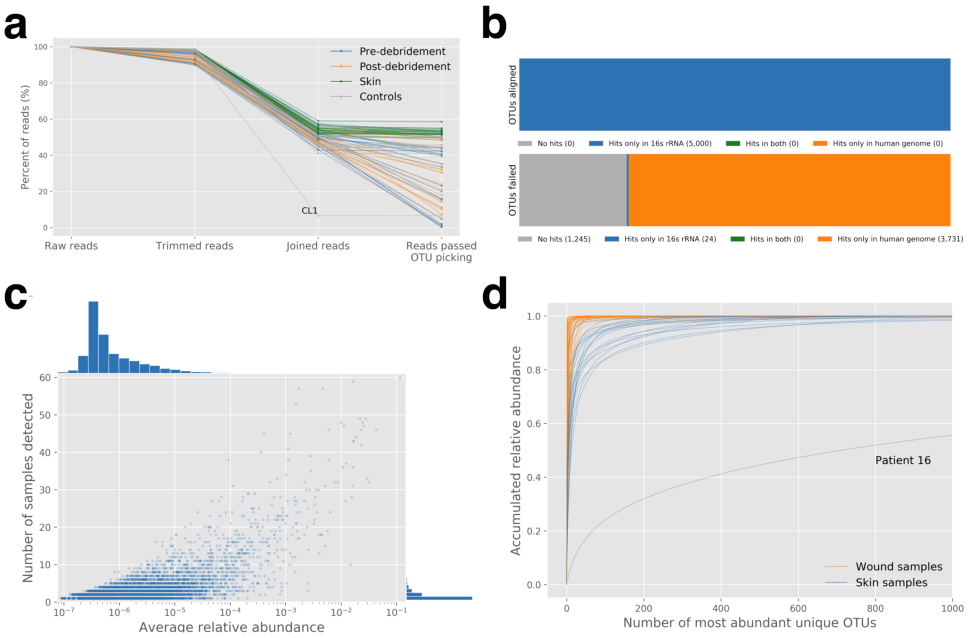
\includegraphics[width=0.9\textwidth]{fig/C3figS1AD.pdf}}
\caption{QIIME pipeline and OTU tables quality control. (A) Percent of reads from each sample passing quality filters in major steps of the QIIME pipeline to prepare the full OTU table. CL1 is the negative control sample collected in the lab. Wound samples have a notably lower percentage of reads passing OTU picking, primarily due to contamination by human DNA. (B) Blastn (2.9.0+) results for representative sequences of OTUs that passed or failed pyNAST alignment (5,000 subsampled OTUs in each case) against NCBI “Human genomic + transcript” and “16S ribosomal RNA sequences (Bacteria and Archaea)” databases. Failed OTUs are primarily human DNA and unmatched sequences to 16S ribosomal RNA database. Number in parentheses indicates the number of OTUs. (C) Distribution of average relative abundance and number of samples in which the OTU was detected, for OTUs in the full OTU table (without pyNAST failures). Bar histograms are shown for average relative abundance and number of samples. (D) Depth of sampling visualized by the cumulative relative abundance composed of the top $k$ most abundant OTUs in each sample. A sample from patient 16 showed insufficient sequencing depth and was excluded from downstream analysis.}
\label{fig:S1AD}
\end{figure}

% fig fka S5 (taxonomic summary boxplot)
\begin{figure}[h]
\centering
\centerline{\includegraphics[width=0.9\textwidth]{fig/C3figS5.pdf}}
\caption{Taxonomic summary of skin and wound microbiota. Taxonomic boxplots of genera with $>0.1$\% average relative abundance, for each sample type. \textit{Staphylococcus} are labelled at the putative species level.}
\label{fig:S5}
\end{figure}

% fig fka s1e (filtering quality control)
\begin{figure}[h]
\centering
\centerline{\includegraphics[width=\textwidth]{fig/C3figS1E.pdf}}
\caption{OTU table filtering retention summary. For some analyses (DESeq2 and BGLMM), the full OTU table was further filtered to include only OTUs present in $>5$ samples with $>10$ counts per sample. Bar chart shows the relative abundance accounted for by OTUs in the filtered table vs. OTUs only present in the full table.}
\label{fig:S1E}
\end{figure}

% fig fka s6 (pearson/spearman correlation plots)
\begin{figure}[h]
\centering
\centerline{\includegraphics[width=\textwidth]{fig/C3figS6ABC.pdf}}
\caption{BGLMM vs. observed data. Comparison of predicted counts under BGLMM and observed counts in all pre-debridement (A), post-debridement (B), and skin (C) samples (except for patient 16). Pearson’s and Spearman’s correlation coefficients are shown. Correlations without over-estimated OTUs whose predictions are above 10-fold of true counts (grey dots) were shown in parentheses to illustrate the effects of outliers. Note that Pearson’s correlation coefficient is sensitive to outliers and, specifically for skin samples, over-estimated counts led to low Pearson’s correlation coefficient. Reasonably robust Spearman’s correlation coefficients shows a good correlation of count rank for OTUs.}
\label{fig:S6}
\end{figure}

% fig fka s7 (composition of associated OTUs)
\begin{figure}[h]
\centering
\centerline{\includegraphics[width=\textwidth]{fig/C3figS7.pdf}}
\caption{Relative abundance of significant OTUs detected using DESeq2 and BGLMM, in pre-debridement vs skin comparison using the filtered OTU table without patient 16. In general, significant OTUs detected using BGLMM constituted a majority of abundance in the wound samples but less abundance in skin samples. On the other hand, significant OTUs detected using DESeq2 had higher relative abundance in skin samples, and composed little abundance (less than 20\%) in some wound samples (patients 2, 4, 11, and 18). Overall, OTUs identified as significant by BGLMM represented $>20$\% of the abundance in all wound samples, while OTUs identified as significant by DESeq2 comprised only a small fraction ($<20$\%) in four wound samples; this greater detection of wound-associated OTUs by BGLMM compared to DESeq2 would be consistent with the ability of BGLMM to account for patient-specific variability.}
\label{fig:S7}
\end{figure}

% fig fka s8 (alpha and beta div of healed/unhealed)
\begin{figure}[h]
\centering
\centerline{\includegraphics[width=\textwidth]{fig/C3figS8AB.pdf}}
\caption{Comparison of healed and non-healing wounds. No difference was found between these groups in alpha diversity measures using Wilcoxon signed-rank tests (A). Within-patient beta diversity measurements (B) show no significant differences in UniFrac distances between samples for healed vs. unhealed wounds using Wilcoxon signed-rank tests.}
\label{fig:S8}
\end{figure}

% fig fka S9ABC (healed/unhealed pre/post oxygen req wilcoxons)
\begin{figure}[h]
\centering
\centerline{\includegraphics[width=\textwidth]{fig/C3figS9ABC.pdf}}
\caption{Oxygen requirement summaries and statistics. Relative abundance boxplots of anaerobes (A) and aerobes (B) in pre- and post-debridement samples, of healed and unhealed wounds. Pre- and post-debridement samples are compared by paired, two-sided Wilcoxon rank-sum tests. Relative abundance of facultative anaerobes in healed or unhealed wounds are compared by two-sided Wilcoxon signed-rank tests (C).}
\label{fig:S9ABC}
\end{figure}

% fig fka s9DE (healed/unhealed taxa box and o2 req dot)
\begin{figure}[h]
\centering
\centerline{\includegraphics[width=\textwidth]{fig/C3figS9DE.pdf}}
\caption{Oxygen requirement summaries and statistics continued. Taxonomic dotplot of average relative abundance of taxa within each outcome, filtered to include taxa with $>0.5$\% average relative abundance (pre- and post-debridement), colored to indicate oxygen requirements (A) and taxonomic boxplots of genera with average relative abundance $>0.1$\%; \textit{Staphylococcus} are labeled at the species level (B).}
\label{fig:S9DE}
\end{figure}

% fig fka s10 (skin OTU associations w/ healing)
\begin{figure}[h]
\centering
\centerline{\includegraphics[width=0.9\textwidth]{fig/C3figS10.pdf}}
\caption{Skin OTUs association with healing status, using DESeq2. OTUs with adjusted $p-$value $<= 0.5$ are shown and the OTU with adjusted $p-$value $< 0.05$ was considered as significant.}
\label{fig:figS10}
\end{figure}

% fig fka s11 (inference robustness w/ or w/o pt 16)
\begin{figure}[h]
\centering
\centerline{\includegraphics[width=0.7\textwidth]{fig/C3figS11.pdf}}
\caption{Robustness of inference to exclusion of patient 16 data. Associations detected in the comparison of pre-debridement vs. skin samples in the filtered OTU table with or without patient 16 using BGLMM (A) or DESeq2 (B). Only significant OTUs with relative abundance $>0.1$\% are shown. Associations detected in the comparison of of pre- vs post- debridement samples in the filtered OTU table with or without patient 16 using BGLMM (C) or DESeq2 (D). Only significant OTUs in the comparison are shown.}
\label{fig:figS11}
\end{figure}

% fig C4 S1 (domain-level taxonomic composition)
\begin{figure}[h]
\centering
\centerline{\includegraphics[width=\textwidth]{fig/C4figS1.pdf}}
\caption{Domain-level taxonomic composition of virome samples. Read abundances in each domain for each sample type, as classified by Kraken2 against the full NCBI refseq database.}
\label{fig:figC4S1}
\end{figure}

% fig C4 S2 (Negative control barcharts)
\begin{figure}[tp]
\centering
\centerline{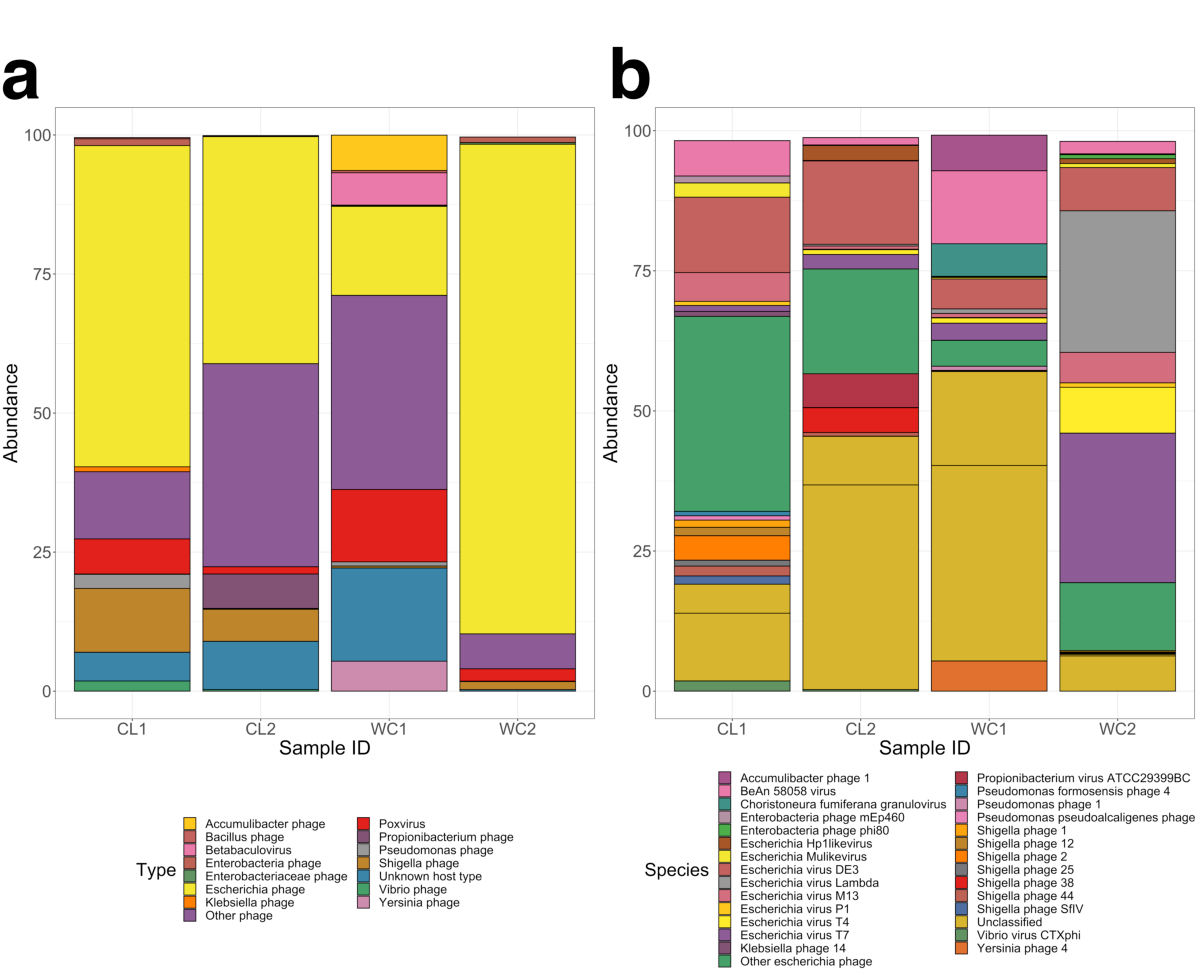
\includegraphics[width=\textwidth]{fig/C4figS2.pdf}}
\caption{Individual negative control sample compositions at type- (a) and species-levels (b); the 30 most species are shown, with two designated as 'unclassified'. The sample source is indicated as 'CL' for the Chen Lab and 'WC' for the wound care center.}
\label{fig:C4S2}
\end{figure}

% fig C4 Sneglist (Contaminant abundance)
\begin{figure}[tp]
\centering
\centerline{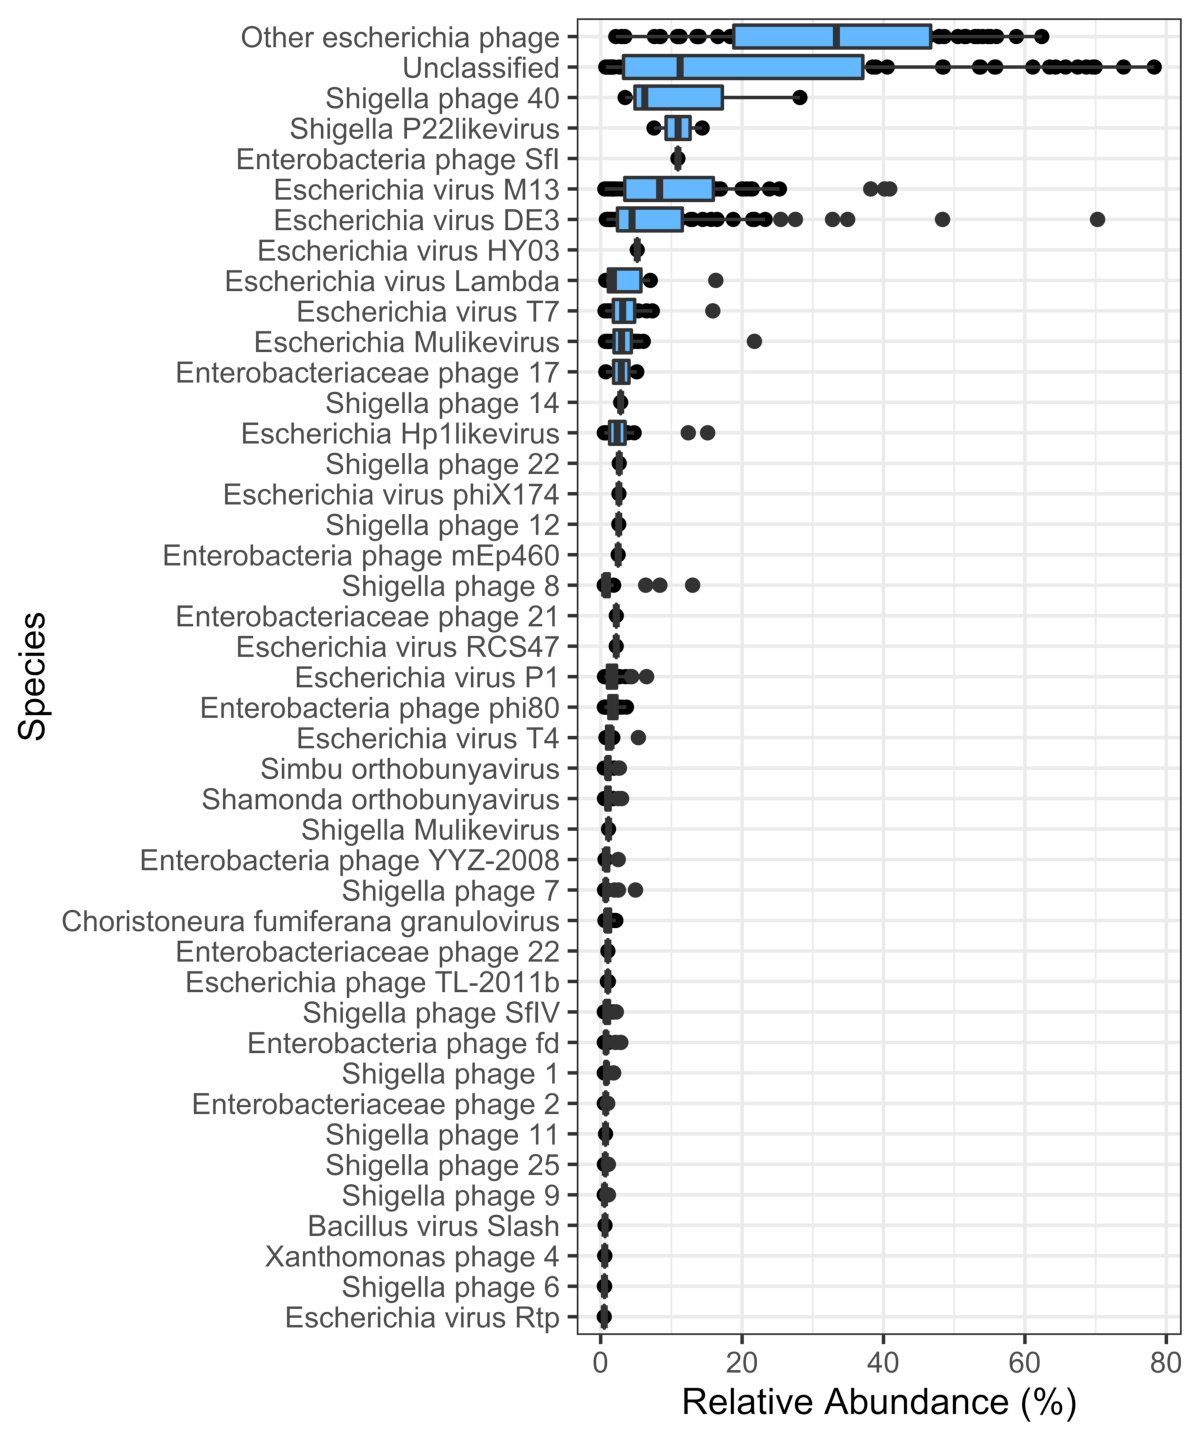
\includegraphics[width=0.9\textwidth]{fig/C4figSneglist.pdf}}
\caption{Contaminant relative abundance prior to decontamination. Taxa displayed were designated as contaminants with relative abundance $>0.5\%$ in $>1$ skin or wound sample prior to decontamination.}
\label{fig:C4Sneglist}
\end{figure}

% fig C4 S3 (decontamination summary)
\begin{figure}[tp]
\centering
\centerline{\includegraphics[width=0.8\textwidth]{fig/C4figS3.pdf}}
\caption{Decontamination summary. Read abundances for each sample, at each step of decontamination (a). Only experimental samples are shown, not negative or positive controls. Contaminant read abundance as a function of extracted DNA concentration, with points colored by sample type, and wound samples from the same patient connected by black lines (b). Overall Spearman correlation coefficient \textit{R} and \textit{p}-value are shown.}
\label{fig:C4S3}
\end{figure}

% fig C4 S4 (Overall taxonomic composition summaries (average) including ambiguous taxa)
\begin{figure}[h]
\centering
\centerline{\includegraphics[width=\textwidth]{fig/C4figS4.pdf}}
\caption{Overall taxonomic composition of skin and wound viromes with unclassified taxa included. Relative abundance of each taxon was averaged across all samples; those with $>0.5\%$ average relative abundance are shown here at the type level (a) and species level (b).}
\label{fig:C4S4}
\end{figure}

% fig C4 S5 (Species-level taxonomic composition)
\begin{figure}[h]
\centering
\centerline{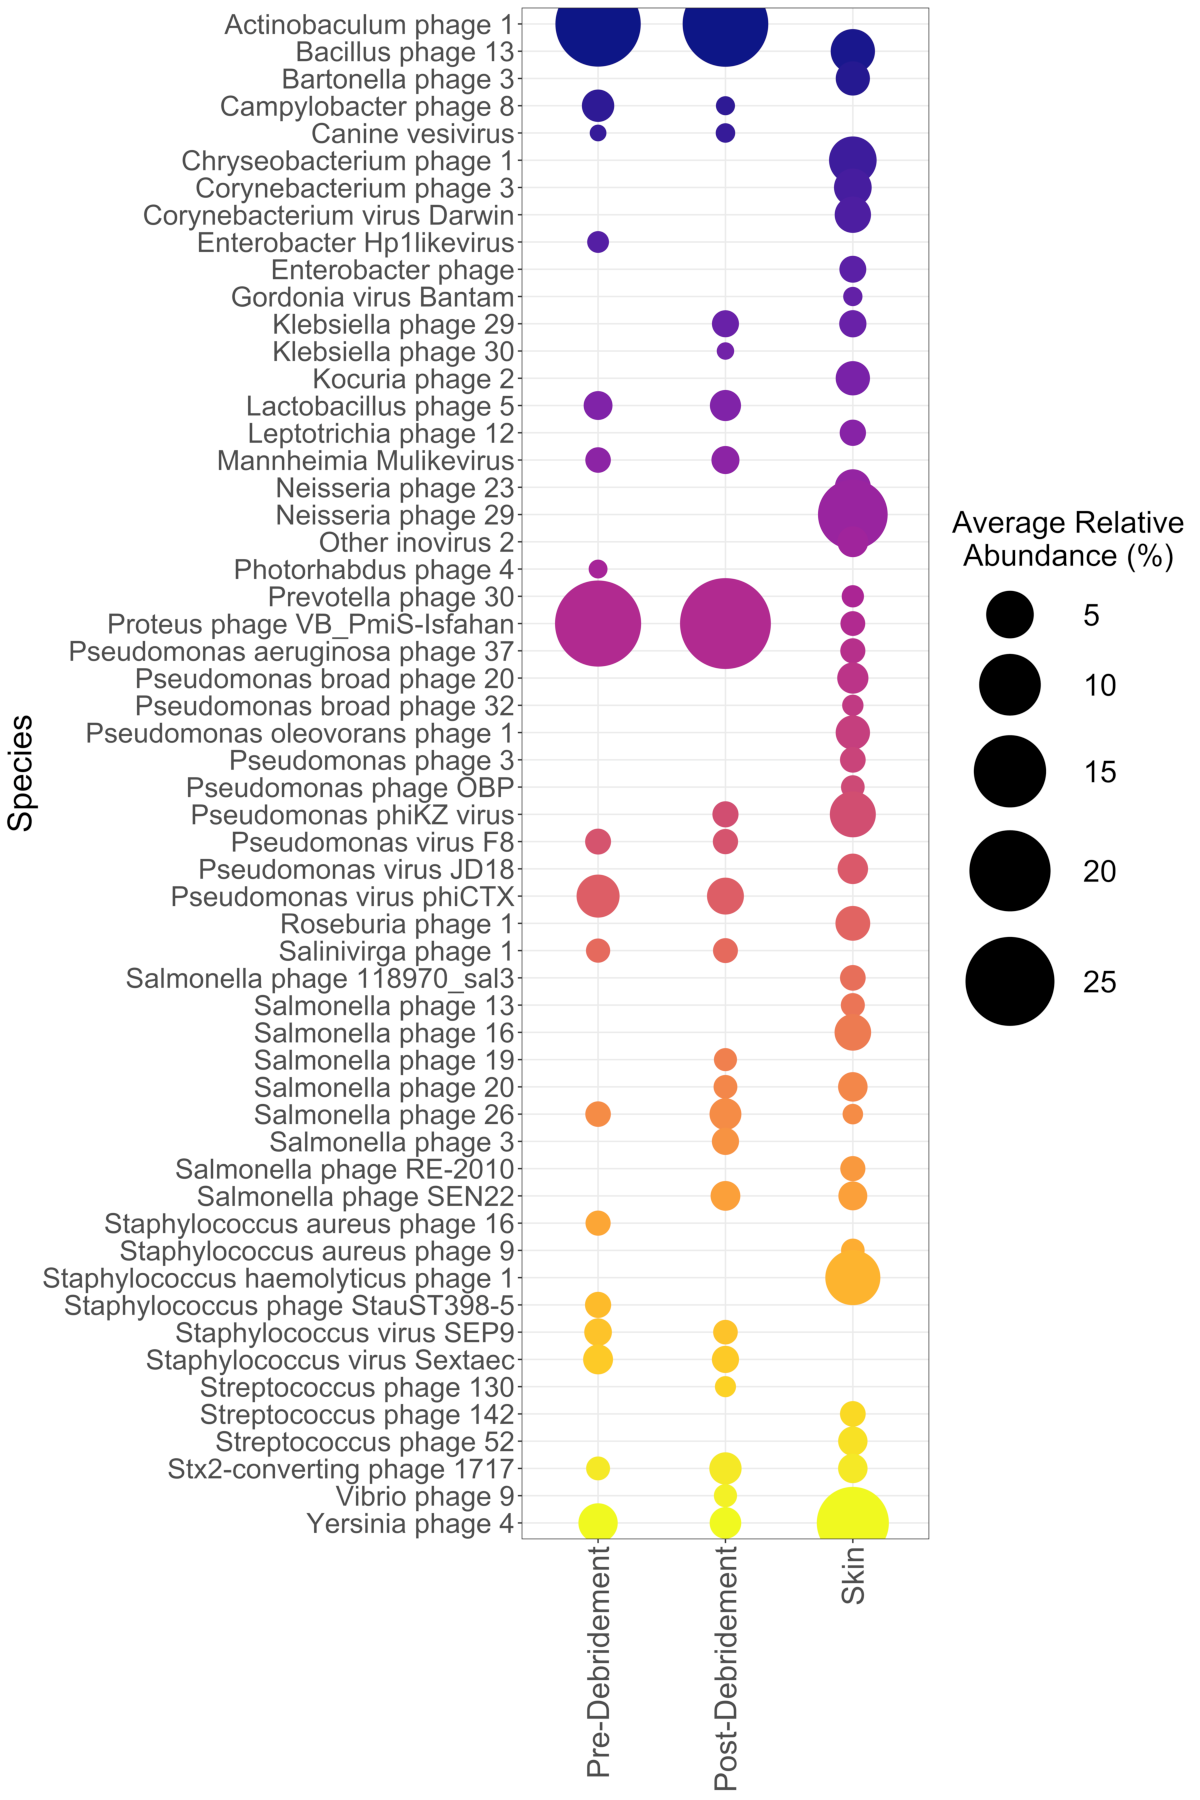
\includegraphics[width=0.8\textwidth]{fig/C4figS5.pdf}}
\caption{Average relative abundance of viral species by sample type. Relative abundances were averaged within pre-debridement, post-debridement, and skin sample types; taxa with average relative abundance $>0.5\%$ are shown.}
\label{fig:C4S5}
\end{figure}

% fig s17 (Skin/wound associations)
\begin{figure}[h]
\centering
\centerline{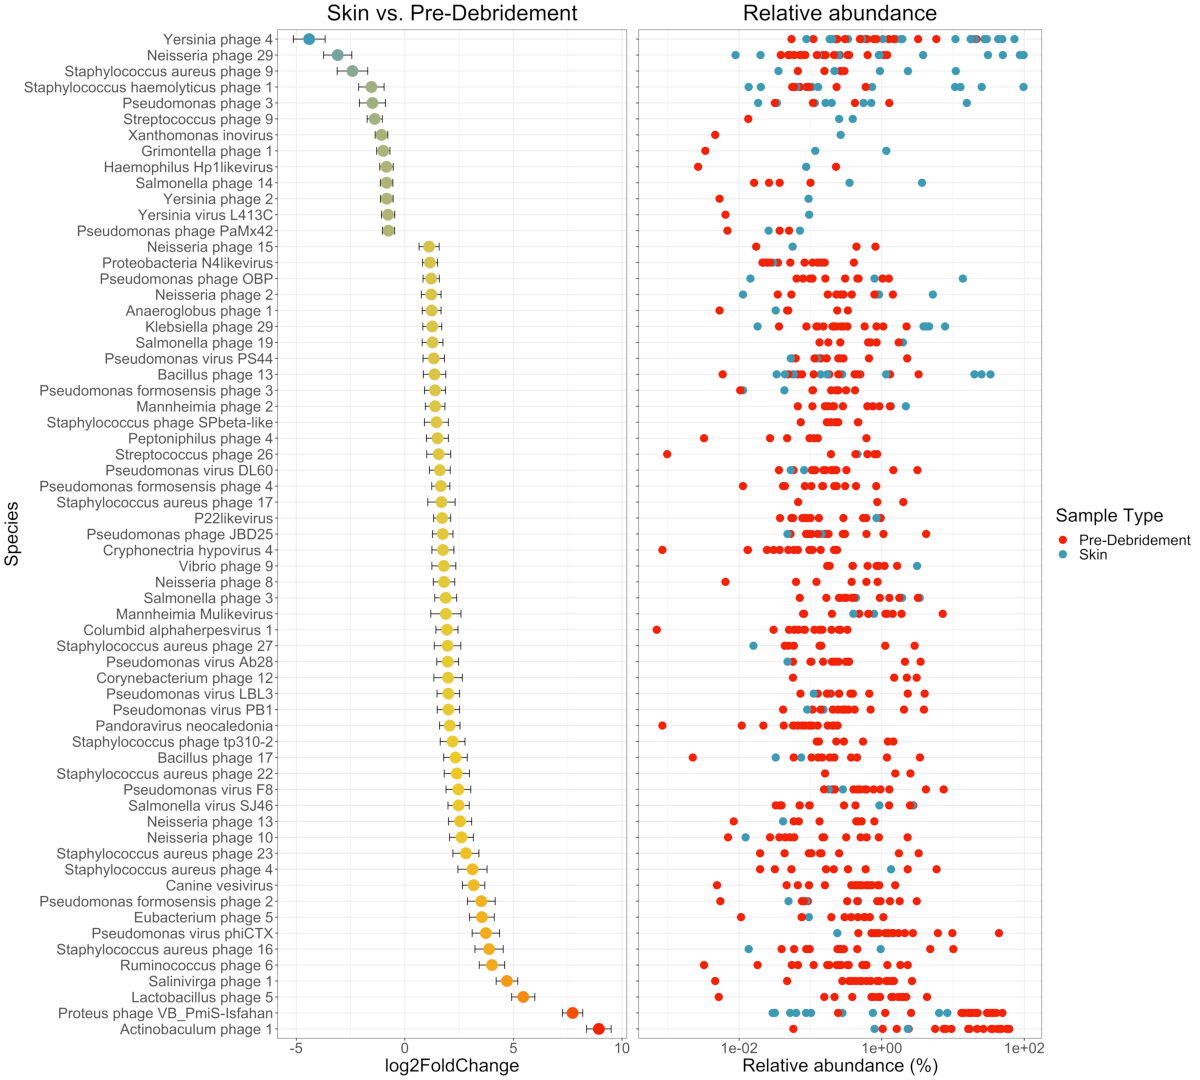
\includegraphics[width=\textwidth]{fig/C4figS6.pdf}}
\caption{Differential abundance analysis of skin and chronic wounds with DESeq2. Associated species are represented by their log2FoldChange from the normalized, geometric mean calculated across all wound samples, contrasting skin (negative change) to wounds (positive change). Error bars represent the log-fold standard error. Only species with adjusted $p\text{-value}<0.05$ are shown. Relative abundance of each associated species, in each sample, are shown on the right; wound samples (pre-debridement) are red, skin samples are blue.}
\label{fig:C4S6}
\end{figure}

\end{subsection}

\clearpage
\begin{subsection}{Discussion of modeling methods}
\label{TextA1}
Both DESeq2 and BGLMM used a generalized linear model with a negative binomial distribution to model OTU counts, and applied shrinkage estimation to enhance prediction accuracy and interpretability of the resulting statistical inferences. However, each method employs a slightly different approach. DESeq2 takes an empirical Bayesian approach that first estimates a normal prior using maximum likelihood estimation on all OTU counts to alleviate false positive detections. It then estimates the covariate effects on abundances of individual OTUs using the empirically estimated normal prior for regression coefficients and performs statistical hypothesis tests based on the large sample approximation to infer differential abundance for fast computation. For BGLMM, we adapted the model in Lee and Sison-Magus \cite{RN33} to take a fully Bayesian approach. BGLMM implements a Bayesian lasso (least absolute shrinkage and selection operator) using a Laplace prior to effectively “shrink” the regression coefficients to zero and produce improved estimates of the covariate effects. In contrast to DESeq2, which assumes the same baseline count of an OTU for all patients, BGLMM accounts for the patient-level heterogeneity in baseline counts of an OTU through patient random effects; heterogeneity of the microbiome among different chronic wounds is observed from our data, and an accommodation of the inter-patient heterogeneity may be important for our study. Indeed, BGLMM showed greater robustness to inclusion or exclusion of a single patient (Figure \ref{fig:figS11}). To fully assess the differences of each method, further computer simulation studies and extended data would be needed. Nevertheless, inferences made in agreement by both statistical techniques are likely to be robust.
\end{subsection}


\end{section}

% fix this later to make it pretty, add the other abbreviations from C3 and C4
\clearpage
\begin{section}{Abbreviations} 
\begin{itemize}
\item[AWS AMI:]	Amazon Web Services Amazon Machine Image
\item[CFU:]	Colony- forming unit
\item[contig:]	Contiguous sequence, assembled from short reads
\item[CTAB:]	Cetyltrimethylammonium bromide
\item[gDNA:]	Genomic DNA
\item[IMG/VR:]	Integrated Microbial Genomes viral analysis database
\item[LB:]	Luria broth
\item[MW:]	Molecular weight
\item[NGS:]	Next-generation sequencing
\item[OD:]	Optical density
\item[OTU:]	Operational taxonomic unit
\item[PS1:]	Pilot study 1, using a standard kit-based extraction
\item[PS2:]	Pilot study 2, using the novel sample preparation
\item[QIIME:]	Quantitative Insights Into Microbial Ecology software
\item[qPCR:]	Quantitative polymerase chain reaction
\item[SDS:]	Sodium dodecyl sulfate
\item[VLP:]	Virus-like particle
\end{itemize}

\end{section}
\end{mainmatter}

%----- Bibliography ----------------
\ssp
\bibliographystyle{JHEP3}
\bibliography{dissertation.enref}

\end{document}
